% Options for packages loaded elsewhere
\PassOptionsToPackage{unicode}{hyperref}
\PassOptionsToPackage{hyphens}{url}
%
\documentclass[
]{book}
\usepackage{amsmath,amssymb}
\usepackage{lmodern}
\usepackage{ifxetex,ifluatex}
\ifnum 0\ifxetex 1\fi\ifluatex 1\fi=0 % if pdftex
  \usepackage[T1]{fontenc}
  \usepackage[utf8]{inputenc}
  \usepackage{textcomp} % provide euro and other symbols
\else % if luatex or xetex
  \usepackage{unicode-math}
  \defaultfontfeatures{Scale=MatchLowercase}
  \defaultfontfeatures[\rmfamily]{Ligatures=TeX,Scale=1}
\fi
% Use upquote if available, for straight quotes in verbatim environments
\IfFileExists{upquote.sty}{\usepackage{upquote}}{}
\IfFileExists{microtype.sty}{% use microtype if available
  \usepackage[]{microtype}
  \UseMicrotypeSet[protrusion]{basicmath} % disable protrusion for tt fonts
}{}
\makeatletter
\@ifundefined{KOMAClassName}{% if non-KOMA class
  \IfFileExists{parskip.sty}{%
    \usepackage{parskip}
  }{% else
    \setlength{\parindent}{0pt}
    \setlength{\parskip}{6pt plus 2pt minus 1pt}}
}{% if KOMA class
  \KOMAoptions{parskip=half}}
\makeatother
\usepackage{xcolor}
\IfFileExists{xurl.sty}{\usepackage{xurl}}{} % add URL line breaks if available
\IfFileExists{bookmark.sty}{\usepackage{bookmark}}{\usepackage{hyperref}}
\hypersetup{
  pdftitle={TILM 3701 - Tilastotiede ja Data 2022},
  pdfauthor={Koonneet; Henri Nyberg; Roope Rihtamo},
  hidelinks,
  pdfcreator={LaTeX via pandoc}}
\urlstyle{same} % disable monospaced font for URLs
\usepackage{longtable,booktabs,array}
\usepackage{calc} % for calculating minipage widths
% Correct order of tables after \paragraph or \subparagraph
\usepackage{etoolbox}
\makeatletter
\patchcmd\longtable{\par}{\if@noskipsec\mbox{}\fi\par}{}{}
\makeatother
% Allow footnotes in longtable head/foot
\IfFileExists{footnotehyper.sty}{\usepackage{footnotehyper}}{\usepackage{footnote}}
\makesavenoteenv{longtable}
\usepackage{graphicx}
\makeatletter
\def\maxwidth{\ifdim\Gin@nat@width>\linewidth\linewidth\else\Gin@nat@width\fi}
\def\maxheight{\ifdim\Gin@nat@height>\textheight\textheight\else\Gin@nat@height\fi}
\makeatother
% Scale images if necessary, so that they will not overflow the page
% margins by default, and it is still possible to overwrite the defaults
% using explicit options in \includegraphics[width, height, ...]{}
\setkeys{Gin}{width=\maxwidth,height=\maxheight,keepaspectratio}
% Set default figure placement to htbp
\makeatletter
\def\fps@figure{htbp}
\makeatother
\setlength{\emergencystretch}{3em} % prevent overfull lines
\providecommand{\tightlist}{%
  \setlength{\itemsep}{0pt}\setlength{\parskip}{0pt}}
\setcounter{secnumdepth}{5}
\usepackage{booktabs}
\usepackage{amsthm}
\usepackage{placeins}
\makeatletter
\def\thm@space@setup{%
  \thm@preskip=8pt plus 2pt minus 4pt
  \thm@postskip=\thm@preskip
}
\makeatother

\usepackage{awesomebox}
\usepackage{color}
\usepackage{framed}
\setlength{\fboxsep}{.8em}

\usepackage{tcolorbox}

\newtcolorbox{blackbox}{
  colback=black,
  colframe=orange,
  coltext=white,
  boxsep=5pt,
  arc=4pt}

%\newenvironment{infobox}[1]
%  {\begin{itemize}
%    \renewcommand{\labelitemi}{
%    \raisebox{-.7\height}[0pt][0pt]{
%      {\setkeys{Gin}{width=3em,keepaspectratio}
%        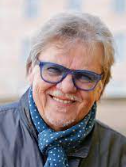
\includegraphics{images/mikko.PNG}}
%    }
%  }
%  \setlength{\fboxsep}{1em}
%  \begin{blackbox}
%  \item}
%  {
%  \end{blackbox}
%  \end{itemize}
%}
\ifluatex
  \usepackage{selnolig}  % disable illegal ligatures
\fi
\usepackage[]{natbib}
\bibliographystyle{apalike}

\title{TILM 3701 - Tilastotiede ja Data 2022}
\author{Koonneet \and Henri Nyberg\footnote{Turun Yliopisto, matematiikan ja tilastotieteen laitos, \href{mailto:henri.nyberg@utu.fi}{\nolinkurl{henri.nyberg@utu.fi}}} \and Roope Rihtamo\footnote{Turun Yliopisto, matematiikan ja tilastotieteen laitos, \href{mailto:roope.rihtamo@utu.fi}{\nolinkurl{roope.rihtamo@utu.fi}}}}
\date{2022-08-23}

\begin{document}
\maketitle

{
\setcounter{tocdepth}{1}
\tableofcontents
}
\hypertarget{kurssin-rakenne}{%
\chapter*{Kurssin rakenne}\label{kurssin-rakenne}}
\addcontentsline{toc}{chapter}{Kurssin rakenne}

\begin{itemize}
\item
  Tällä kurssilla tarkoituksena on melko yleisellä tasolla johdatella tilastotieteen ja aineistojen (datan) maailmaan pohtimalla myös näiden laajempia merkityksiä tieteellisen tutkimuksen hyvin keskeisinä osina.
\item
  Kurssilla vältetään, mahdollisuuksien mukaan, kovin teknistä matemaattista esitystapaa, mutta tarvittavissa määrin tullaan myös käyttämään tilastotieteen perusopinnoissa tarvittavia matemaattisia merkintöjä ja määritelmiä. Esim. todennäköisyyslaskennan ja tilastollisen päättelyn perusteita ei käydä vielä riittävällä matemaattisella tarkkuudella lävitse, vaan nämä tarkastelut jäävät tätä kurssia seuraavien kurssien (\href{https://opas.peppi.utu.fi/fi/opintojakso/TILM3553/1734?period=2022-2024}{TILM3553 Todennäköisyyslaskennan peruskurssi} tai \href{https://opas.peppi.utu.fi/fi/opintojakso/TILM3568/3385?period=2022-2024}{TILM3568 Todennäköisyyslaskenta sivuaineopiskelijoille} sekä \href{https://opas.peppi.utu.fi/fi/opintojakso/TILM3555/1731?period=2022-2024}{TILM3555 Tilastollisen päättelyn peruskurssi}) asiaksi. Nämä kurssit, yhdessä alkuvaiheen pakollisten matematiikan kurssin lisäksi, muodostavat siis tämän kurssin johdannon kanssa lähtökohdan tilastotieteen opinnoille.
\item
  Luennot eivät suoraan perustu yhteen kirjaan tai lähteeseen. Käytettyjä lähdemateriaaleja luetellaan alapuolella oheislukemiston myötä.
\item
  Oheislukemistoa (sopivilta osin):

  \begin{itemize}
  \tightlist
  \item
    Mellin, I. (2004). Johdatus tilastotieteeseen: Tilastotieteen johdantokurssi (1.kirja). Yliopistopaino, Helsingin yliopisto.
  \item
    Mellin, I. (2000). Johdatus tilastotieteeseen: Tilastotieteen jatkokurssi (2.kirja). Yliopistopaino, Helsingin yliopisto.
  \item
    Mellin, I. (2006). Tilastolliset menetelmät. Luentomoniste, Aalto yliopisto (TKK).
  \item
    Holopainen, M. ja P. Pulkkinen (2008). Tilastolliset menetelmät. Sanoma Pro Oy.
  \item
    Pahkinen, E. ja R. Lehtonen (1989). Otanta-asetelmat ja tilastollinen analyysi. Gaudeamus, Helsinki.
  \item
    Pahkinen, E. ja R. Lehtonen (2004). Practical Methods for Design and Analysis of Complex Surveys. 2. painos, Wiley.
  \item
    Sund, R. (2003). Tilastotiede käytännön tutkimuksessa -kurssi. Helsingin yliopisto.
  \item
    Silver, N. (2014). Signaali ja kohina: Miksi monet ennusteet epäonnistuvat mutta jotkin eivät? Terra Cognita. (Suomentanut Kimmo Pietiläinen)

    \begin{itemize}
    \tightlist
    \item
      Englanninkielinen teos: Silver, N. (2015). The Signal and the Noise: Why So Many Predictions Fail--but Some Don't. Penguin Books; Illustrated edition
    \end{itemize}
  \item
    Pesonen, M. (2017). Kurssimateriaali kurssille Aineistonhankinta ja tutkimusasetelmat, Turun yliopisto.
  \item
    Vartia, Y. (1989). Tilastotieteen perusteet. Yliopistopaino, Helsinki. II painos.
  \end{itemize}
\item
  Muita taustamateriaaleja

  \begin{itemize}
  \tightlist
  \item
    \href{https://tilastokoulu.stat.fi/verkkokoulu_v2.xql?course_id=tkoulu_tilaj\&lesson_id=1\&subject_id=0\&page_type=sisalto}{Tilastokeskuksen tilastokoulu (linkki)}
  \item
    Tilastotieteen sanasto suomi-englanti-suomi, ks. Juha Alho, Elja Arjas, Esa Läärä ja Pekka Pere (2021). \href{https://tilastoseura.fi/}{Tilastotieteen sanasto. Suomen Tilastoseuran julkaisuja 8.}
  \end{itemize}
\end{itemize}

Suuret kiitokset Visa Kuntzelle ja Emil Lehdelle kommenteista ja avusta materiaalin työstämisessä. Kaikki jäljelle jääneet painovirheet ovat materiaalin kokoajien.

\hypertarget{johdantoa-ja-johdattelua-tilastotieteeseen}{%
\chapter{Johdantoa ja johdattelua tilastotieteeseen}\label{johdantoa-ja-johdattelua-tilastotieteeseen}}

\emph{Ihmisellä on luontainen pyrkimys ymmärtää, mitä hänen ympärillään tapahtuu. Ymmärrys perustuu ihmisen tekemiin havaintoihin, joita luokittelemalla tai seuraamalla hän pyrkii löytämään säännönmukaisuuksia. Näiden säännönmukaisuuksien löytäminen vaatii loogisten johtopäätösten tekoa. Pelkän uteliaisuuden tyydyttämiseen ja älyllisen mielihyvän lisäksi ihminen pyrkii ennakoimaan tulevaa ja siten varautumaan tuleviin tapahtumiin\ldots{} Edellä kuvattuja taitoja voi oppia.}

Holopainen ja Pulkkinen, 2008

\hypertarget{tilastotiede-ja-kurssin-idea}{%
\section{Tilastotiede ja kurssin idea}\label{tilastotiede-ja-kurssin-idea}}

\begin{itemize}
\tightlist
\item
  Tämän tilastotieteen ensimmäisen kurssin ideana on (ainakin)

  \begin{itemize}
  \tightlist
  \item
    Esitellä ja johdatella \textbf{tilastolliseen ja tieteelliseen ajatteluun} ja sen hyödyntämiseen eri tyyppisissä tutkimusongelmissa.
  \item
    Esitellä tilastotieteen roolia \textbf{empiirisen tutkimusaineiston keräämisessä ja analyysissä} sekä tarkastella tieteentekemisen ja tilastotieteen suhdetta.
  \item
    Pohtia \textbf{tilastotieteen olemusta tieteenalana} ja tarkastella tilastotieteen ja datatieteiden (data sciencen) samankaltaisuuksia ja eroja.
  \item
    Pohtia \textbf{sattuman ja satunnaisuuden roolia} jokapäiväisessä elämässä ja erityisesti osana tieteellistä tutkimusprosessia.
  \item
    Oppia tilastotieteen peruskäsitteitä ja (tilastollisen) tutkimuksenteon alkeita ja siihen liittyviä mahdollisia ongelmia esimerkiksi tilastollisten aineistojen keräämisessä.
  \item
    Oppia tilastollisten aineistojen \textbf{kuvaamisen ja käsittelyn} alkeita sekä tilasto(tieteellisen)llisen \textbf{mallintamisen} ja \textbf{koeasetelmien} peruskäsitteitä.
  \end{itemize}
\end{itemize}

\vspace{0.75cm}

\begin{itemize}
\tightlist
\item
  Kurssilla käsitellään myös \textbf{tilastollisen päättelyn} peruskäsitteitä ja perusteita kuten

  \begin{itemize}
  \tightlist
  \item
    Mitä on \textbf{todennäköisyys} ja miten sen tulkitaan tilastotieteessä sekä laajemmin tieteessä. Erityisesti tilastotieteen osalta keskiössä on tämän kurssin osalta \textbf{satunnaismuuttujat} sekä niihin liitettävät käsitteet

    \begin{itemize}
    \tightlist
    \item
      \textbf{Odotusarvo}, \textbf{varianssi} ja kahden (tai useamman) satunnaismuuttujan \textbf{korrelaatio}.
    \item
      Satunnaismuuttujien \textbf{todennäköisyysjakaumien} perusteita ja niiden yhteyksiä mm. normaalijakaumaan ja muutamiin muihin keskeisiin jakaumiin.
    \item
      Tilastollinen malli työkaluna satunnaismuuttujien formaalissa mallintamisessa ja päättelyssä. Tilastollisen malliin liittyy (usein) \textbf{parametreja} joihin tilastollinen päättely kohdistuu.
    \item
      Tilastollisten mallien \textbf{estimoinnin} perusidea, eli miten tilastollisen mallin parametreille muodostetaan arvot käytettävissä olevan aineiston pohjalta. Esimerkiksi: mitä tarkoittaa tilastollisen mallin parametrin \textbf{estimaattori} ja sen \textbf{harhattomuus}?
    \item
      Alustavia tarkasteluja tilastollisen mallin uskottavuuden käsitteelle ja \textbf{luottamusväleille} tilastollisen mallin estimoiduille parametreille.
    \end{itemize}
  \end{itemize}
\end{itemize}

\vspace{0.75cm}

\begin{itemize}
\tightlist
\item
  Toinen kurssin keskeisistä teemoista on tarkastella tieteellistä tutkimusprosessia teoriassa ja käytännössä. Tämä sisältää mm. seuraavia aiheita (joita siis käsitellään tällä kurssilla päällisin puolin ja varsin yleisestä näkökulmasta katsoen): tarkemmat yksityiskohdat jäävät tätä kurssia seuraavien tilastotieteen kurssien aihepiireiksi):

  \begin{itemize}
  \tightlist
  \item
    \textbf{Tutkimusongelman} asettaminen: mitä halutaan tutkia?\\
  \item
    Tutkimusongelman täsmentäminen ja \textbf{tutkimusstrategian} laatiminen: millä keinoin asetettuun tutkimusongelmaan voidaan vastata?
  \item
    \textbf{Tutkimusaineiston} (tai vain lyhyemmin \textbf{aineiston} eli \textbf{datan}) kerääminen

    \begin{itemize}
    \tightlist
    \item
      \textbf{Aineiston ennakkoehdot}: mitkä ehdot tulee täyttyä, jotta asetettuun tutkimusongelmaan voidaan vastata?
    \item
      \textbf{Otanta} (ja mittaaminen): miten tutkimusaineisto kerätään niin, että se täyttää aineiston ennakkoehdot? Erilaisissa tutkimuksissa käytetään erilaisia aineistoja kuten:

      \begin{itemize}
      \tightlist
      \item
        Survey- ja rekisteriaineistot
      \item
        Havaintoarvojen välistä korrelaatiota esiintyy mm. aikasarja-aineistojen tai pitkittäisaineistojen tapauksessa
      \end{itemize}
    \end{itemize}
  \end{itemize}
\item
  \textbf{Aineiston kuvaaminen}: minkälaista aineistoa on kerätty ja vastaako se ennakkoehtoja?
\item
  \textbf{Aineiston analyysin} lähtökohtia

  \begin{itemize}
  \tightlist
  \item
    Mitä tilastollista mallia/malleja käytetään?
  \item
    Mitä tarkoitetaan mallien tuntemattomien parametrien arvojen estimoinnilla?
  \item
    Tilastollinen päättely (estimointitulosten pohjalta)
  \end{itemize}
\item
  \textbf{Johtopäätelmien} tekeminen tilastollisen päättelyn pohjalta: saatiinko tutkimusongelmaan vastaus ja kuinka luotettava saatu vastaus on?
\end{itemize}

\hypertarget{tilastotieteen-asema-tutkimusyhteisuxf6n-ulkopuolella}{%
\section{Tilastotieteen asema tutkimusyhteisön ulkopuolella}\label{tilastotieteen-asema-tutkimusyhteisuxf6n-ulkopuolella}}

\begin{itemize}
\tightlist
\item
  Tilastotiede on oppiaineena usein varsin tuntematon toisen asteen opinnoista valmistuneelle, sillä sitä ei juurikaan opeteta lukioissa tai ammattikouluissa huolimatta sen keskeisestä ja kasvavasta roolista tiedemaailman kentillä.
\item
  Tiedeyhteisön ulkopuolellakin \textbf{tilastotiedettä ja tilastotieteilijöitä arvostetaan laajalti}.
\item
  \textbf{Tilastotiede onkin nostanut profiiliaan viimeisten vuosikymmenien aikana} tietoteknisen kehityksen tuotua laajat tietoaineistot ja kehittyneet laskennalliset menetelmät lähes jokaisen kansalaisen saataville.
\item
  Tämä ``datavallankumous'' näkyy tilastotieteilijöiden kysynnässä työmarkkinoilla: erilaisten aineistojen määrän lisääntyessä kasvaa myös kysyntä työntekijöistä, jotka osaavat ammatitaitoisesti käsitellä, tulkita ja mallintaa tilastollisia aineistoja.
\item
  Ei siis liene ihmekään, että erilaisten ``data''-alkuisten työpaikkojen, kuten \textbf{datatieteilijä} (eng. \textbf{data scientist}) tai \textbf{data-analyytikko} ( \textbf{data-analyst}) määrä on kasvanut voimakkaasti jo pidempään. Kaikkia tieto- ja datainensiivisten ammattien tekijöitä yhdistää yksi tekijä: \textbf{heidän tulee hallita ja osata tilastotiedettä!} Karkeistettuna mitä paremmin ja enemmän (laajemmin), sen parempi palkka ja monipuolisemmat työtehtävät!
\end{itemize}

\hypertarget{kurssin-luonne-tilastotieteen-ja-datatieteendata-analytiikan-opintojen-esittelijuxe4nuxe4}{%
\section{Kurssin luonne tilastotieteen (ja datatieteen/data-analytiikan) opintojen esittelijänä}\label{kurssin-luonne-tilastotieteen-ja-datatieteendata-analytiikan-opintojen-esittelijuxe4nuxe4}}

Kurssin mittaan esitellään tilastotieteen perusteiden lisäksi \textbf{miten TY:ssa tilastotieteen opinnoissa syvennytään} tällä kurssilla esiteltäviin menetelmiin, aineistotyyppeihin ja mallinnuskokonaisuuksiin.

\hypertarget{luku2}{%
\chapter{Tieteellinen tieto, tilastot ja arkitieto yhteiskunnassa}\label{luku2}}

\hypertarget{alaluku21}{%
\section{Mitä on tiede?}\label{alaluku21}}

\hypertarget{alaluku22}{%
\section{Tieteellinen menetelmä}\label{alaluku22}}

\hypertarget{alaluku23}{%
\section{Tilastojen yleisestä roolista yhteiskunnassa}\label{alaluku23}}

\hypertarget{alaluku24}{%
\section{Mitä on tutkimus?}\label{alaluku24}}

\hypertarget{alaluku25}{%
\section{Tieteellisen tutkimuksen vaiheet ja tulosten julkaiseminen}\label{alaluku25}}

\hypertarget{tilastotiede-tieteenalana}{%
\chapter{Tilastotiede tieteenalana}\label{tilastotiede-tieteenalana}}

Tässä luvussa hahmottelemme tilastotieteen piirteitä tieteenalana. Käymme läpi tilastotieteelle
ominaisia piirteitä, jotka erottavat sen niin lähitieteistä, kuten matematiikasta ja tietojenkäsit-
telytieteestä, kuin myös sovellusaloista. Usein näkee tilastotieteen typistettävän vain työkaluksi
eri sovellusalojen empiiriseen tutkimukseen siitäkin huolimatta että tilastotieteellä on oma rikas
teoriapohjansa sekä kiistaton asema omana tieteenalanaan.
Tieteenalan määritteleminen lyhyesti on aina hieman hankalaa. Tästä huolimatta seuraavassa
yritämme osaltaan vastata seuraaviin kysymyksiin:

\begin{itemize}
\tightlist
\item
  Mitä tilastotiede on ja mitä se ei ole? Miksi tilastotiede ei ole vain sovellettua matematiikkaa
  tai matematiikalla höystettyä tietojenkäsittelyä?
\item
  Mihin tilastotiedettä käytetään? Onko tilastotieteellä käyttöä ns. ``akatemian'' eli tutki-
  musyhteisön ulkopuolella?
\item
  Tilastotieteelle tyypillistä kritiikkiä?
\end{itemize}

\hypertarget{lisuxe4uxe4-tilastotieteen-perustermejuxe4}{%
\section{Lisää tilastotieteen perustermejä}\label{lisuxe4uxe4-tilastotieteen-perustermejuxe4}}

Seuraavia tilastotieteen esittelyä ja karakterisointeja ajatellen määritellään seuraavassa lisää tilastotieteellisen tutkimuksen peruskäsitteitä. Näihin käsitteisiin paneudutaan osaltaan tarkemmin mm. luvussa ?? {[}otantaluku{]}.

\begin{itemize}
\tightlist
\item
  Tilastotieteellinen tutkimus tarkastelee reaalimaailman ilmiöitä. Täten tutkimuskohteena on tavallisessa elämässä tavattavia asioita, ihmisiä tai tapahtumia. Tutkimuskohteita kutsutaan tilastoyksiköiksi ja niiden joukkoa kutsutaan populaatioksi (perusjoukoksi). Esimerkiksi jos tutkitaan kuntavaaleissa äänestävien tuloja niin jokainen äänestysikäinen muodostaa oman tilastoyksikkönsä (ks. alla) ja täten populaationa (perusjoukkona) toimii kaikki
  äänestysikäiset kansalaiset. Jos taas tutkitaan äänestysaktiivisuutta eri kunnissa, muodostaa jokainen kunta oman tilastoyksikkönsä ja kaikki Suomen kunnat muodostavat populaation.
\end{itemize}

\begin{noteblock}{}
\textbf{Populaatio}

Konkreettinen tai hypoteettinen tutkimuskohteiden joukko, joka
koostuu kaikista tilastoyksiköistä

\end{noteblock}

\begin{itemize}
\item
  Populaation muodostavilta tilastoyksiköiltä tarkastellaan niiden ominaisuuksia, eli \textbf{tilastollisia muuttujia}. Edellisissä esimerkeissä nämä olisivat esim. äänestäjien tulot ja kuntien äänestysprosentti. Mielenkiinnon kohteena olevia tilastollisia muuttujia kutsutaan \textbf{tutkimusmuuttujiksi} (tulot ja kuntien äänestysprosentti) ja niiden lisäksi voidaan kerätä ylimääräistä tietoa eli \textbf{taustamuuttujia} (näitä voisi olla esimerkiksi asuinpaikka ja kunnan väkiluku).
\item
  Tilastoyksiköiden tilastollisilla muuttujilla on tietty mahdollisten arvojen joukko, ja näillä arvoilla on jokin \textbf{jakauma} populaatiossa. Esimerkiksi tulot voivat määritelmästä riippuen saada minkä tahansa positiivisen arvon mutta äänestysprosentti on luonnollisesti rajattu nollan ja sadan prosentin väliin.
\end{itemize}

\begin{noteblock}{}
\textbf{Tilastoyksikkö ja tilastollinen muuttuja}

Populaation muodostavilta tilastoyksiköiltä (populaation alkioilta) tarkastellaan tilastollisia muuttujia, joita voidaan mitata tai havaita.

\end{noteblock}

\begin{itemize}
\tightlist
\item
  Kun tarkasteltavien tilastoyksikön tilastollisten muuttujien (numeeriset) arvot havaitaan, kutsutaan näiden arvojen joukkoa \textbf{havainnoksi}
\end{itemize}

\begin{noteblock}{}
\textbf{Havainto}

Havainto muodostuu tilastoyksikön tarkasteltavien tilastollisten muuttujien havaitusta arvoista.

\end{noteblock}

\begin{itemize}
\item
  Populaatio koostuu tilastoyksiköistä, joilla on tilastollisia muuttujia. Tarkasteltavista tilastollisista muuttujista kerätään havaintoja, joiden pohjalta tutkitaan \textbf{populaation ominaisuuksia}.
\item
  Kerättyjen havaintojen joukko muodostaa \textbf{havaintoaineiston}, eli \textbf{datan}.
\end{itemize}

\begin{noteblock}{}
\textbf{Havaintoaineisto/data}

Havaintoaineisto, data, on tilastoyksiköiden tilastollisista muuttujista kerätty havaintojen joukko.

\end{noteblock}

\textbf{Tiivistettynä}:

\begin{itemize}
\tightlist
\item
  Populaatio tutkimuksen kohteena olevia tilastoyksiköitä.
\item
  Havaitaan tilastoyksiköistä tutkimuksen kannalta mielenkiintoisia tilastollisten muuttujien numeerisia arvoja.
\item
  Nämä havainnot muodostavat havaintoaineiston, eli datan, jota voidaan käyttää tutkimuksessa.
\end{itemize}

-- Terminologiaa (käydään vielä läpi tarkemmin jatkossa):
- Tilastoala = Tilastotiede + Tilastotoimi
- Tilastotiede = Teoreettinen tilastotiede + Soveltava tilastotiede
- Tilastotoimi = Tilastojen tuotanto + Tilastojen hyödyntäminen

\hypertarget{mituxe4-tilastotiede-on-ja-mituxe4-se-ei-ole}{%
\section{Mitä tilastotiede on ja mitä se ei ole?}\label{mituxe4-tilastotiede-on-ja-mituxe4-se-ei-ole}}

\begin{itemize}
\tightlist
\item
  Aloitetaan tarkastelemalla erinäisiä \textbf{tilastotieteen ``karakterisointeja''} eri tahojen ja tutkijoiden toimesta:

  \begin{itemize}
  \tightlist
  \item
    \textbf{\emph{Tilastotiede on tietotuotannon teknologiaa}}, \emph{jonka avulla voidaan suorittaa kvantitatiivisten tietojen joukkotuotantoa ja havaintoihin perustuvia tieteellisiä ja käytännöllisiä päätöksiä. Tilastotiede on siis yksikköjen muodostamaan joukkoon liittyvän numeerisen tietoaineiston keräämistä, analysointia ja tulkintaa koskeva tiede} \footnote{\href{https://fi.wikipedia.org/wiki/Leo_T\%C3\%B6rnqvist}{Leo Törnqvistin}, Suomen ensimmäisen tilastotieteen professorin, esittämä luonnehdinta (Vartia, 1989).}.
  \item
    \textbf{\emph{Tilastotiede on yleinen menetelmätiede}}, \emph{jota sovelletaan, jos reaalimaailman ilmiöstä halutaan tehdä johtopäätöksiä ilmiötä kuvaavien kvantitatiivisten tai numeeristen tietojen perusteella sellaisissa tilanteissa, joissa tietoihin liittyy epävarmuutta tai satunnaisuutta} \footnote{Mellin, (2005).}.
  \item
    \textbf{\emph{Tilastotiede on yleinen menetelmätiede}}, \emph{jota sovelletaan, jos reaalimaailman ilmiöstä halutaan tehdä johtopäätöksiä ilmiötä kuvaavien kvantitatiivisten tai numeeristen tietojen perusteella sellaisissa tilanteissa, joissa tietoihin liittyy epävarmuutta tai satunnaisuutta.}
  \item
    \emph{Vale, emävale, tilasto} \footnote{\href{https://fi.wikipedia.org/wiki/Mark_Twain}{Mark Twain} popularisoi tämän lausahduksen teoksessaan \emph{Chapters from My Autobiography} jo vuonna 1907.}.
  \item
    \emph{Statistics concerns what can be learned from data} \footnote{(A.C. Davison)}.
  \item
    \emph{``Maalaisjärjen tehostamista''} \footnote{(Sund, 2003)}.
  \end{itemize}
\item
  Tilastotiede siis \textbf{kehittää} ja \textbf{soveltaa menetelmiä} ja (tilastollisia) \textbf{malleja}, joiden avulla reaalimaailman ilmiöistä voidaan tehdä johtopäätöksiä ilmiöitä kuvaavien numeeristen tai kvantitatiivisten tietojen perusteella tilanteissa, joissa tietoihin liittyy \textbf{epävarmuutta ja satunnaisuutta}.

  \begin{itemize}
  \tightlist
  \item
    Tilastollisten menetelmien avulla pyritään löytämään reaalimaailman satunnaisia ilmiöitä kuvaavista numeerisista (eli kvantitatiivisista) tiedoista \textbf{systemaattisia piirteitä} joita jalostetaan sellaiseen muotoon, että ilmiöistä voidaan tehdä päätelmiä.

    \begin{itemize}
    \tightlist
    \item
      Vrt. signaalin ja kohinan erottaminen (ks. Silver, 2014).
    \end{itemize}
  \item
    Tilastolliset mallit perustuvat todennäköisyyslaskentaan ja niillä mallinnetaan reaalielämän ilmiöiden alla piileviä prosesseja tai mekanismeja. Näiden prosessien tuottamia tietoja (aineistoja) tiivistetään usein graafisiksi esityksiksi ja tunnusluvuiksi sekä tilastollisten mallien parametreiksi, joiden pohjalta johtopäätöksiä tehdään.
  \item
    Tässä onnistuakseen tilastollisten menetelmien tuleekin pyrkiä erottelemaan \textbf{sattuma} ja \textbf{systemaattisuus} tarkasteltavissa ilmiöissä tai, tarkemmin, niitä kuvaavissa aineistoissa, jotta johtopäätökset olisivat luotettavia.
  \end{itemize}
\end{itemize}

\textbf{Voidaan sanoa, että saadakseen tarkemmin selville mitä tilastotiede on, pitää opiskella tilastotiedettä ja sen käyttöä!}

\begin{itemize}
\item
  Edellisten tilastotieteen yleismaailmallisten luonnehdintojen jälkeen onkin sopivaa kysyä \textbf{mitä tilastotiede ei ole}.

  \begin{itemize}
  \tightlist
  \item
    Vaikka sana \textbf{tilasto} tuo useimmille ensimmäisenä mieleen yhteiskuntaa ja sen toimintaa kuvaavat \textbf{numeeristen tietojen järjestelmälliset kokoelmat}, tilastotiede ei suinkaan ole ainoastaan tilastojen ja niiden tekemisen oppia.

    \begin{itemize}
    \tightlist
    \item
      Tämä siitäkin huolimatta, että niiden menetelmien konstruointi, joilla näitä tilastoja tuotetaan, jalostetaan ja analysoidaan on keskeinen osa tilastotiedettä. Tilastot ovat siis usein tilastotieteen soveltajan tutkimuskohteena ja tilastojen laadinnassa käytetään apuna tilastotieteen menetelmiä.
    \item
      Suomessa \href{https://www.stat.fi/}{Tilastokeskus} toimii virallisena tilastoviranomaisena ja tilastotuottajana. Tätä \textbf{tilastotuotannon} kokonaisuutta nimitetään ajoittain \textbf{tilastotoimeksi}. \textbf{Tilastotieteen käyttöalue on paljon tätä laajempi}.
    \end{itemize}
  \item
    Tilastotieteen kannalta mikä tahansa reaalimaailman ilmiötä kuvaava \textbf{numeeristen tai kvantitatiivisten tietojen järjestelmällinen kokoelma} voi muodostaa \textbf{tilastollisen aineiston} ja siten tilastollisen tutkimuksen mahdollisen kohteen.
  \item
    Esimerkiksi kaikki \textbf{empiirisen} tai \textbf{kvantitatiivisen}
    tutkimuksen tutkimus- tai havaintoaineistot ovat tilastotieteen kannalta tilastollisia aineistoja.
  \end{itemize}
\item
  Tilastotiede sijoittuu tieteiden kentässä matematiikan, filosofian ja tietojenkäsittelytieteen rinnalle. Tästä huolimatta se ei kuitenkaan ole yksiselitteisesti minkään näiden osa-alue.

  \begin{itemize}
  \tightlist
  \item
    \textbf{Tilastotiede ei ole matematiikan osa-alue}, sillä tilastotiede lähestyy tieteellistä ongelmanratkaisua eri tavoin: matematiikka on tietyllä tavallaan aina eksaktia ja sen tulokset perustuvat formaaliin deduktioon ja loogisiin todistuksiin, johtaen usein ``eksaktiin'\,' ratkaisuun tai matemaattisesti formaaliin ratkaisun esitystapaan. Tilastotiede sen sijaan on aina konteksti- ja aineistopohjaista ja perustuu induktiiviseen päättelyyn. Saadut tulokset ovat aina epävarmoja - koska ne kuvailevat epävarmaa tietoa generoivia prosesseja!

    \begin{itemize}
    \tightlist
    \item
      Tilastotiede on siis hyvä nähdä omana tieteenalanaan matemaattisesta esitystavastaan huolimatta. Eihän esimerkiksi myöskään fysiikkaa (sentään) pidetä matematiikan osa-alueena!
    \end{itemize}
  \item
    \textbf{Tilastotiede ei ole myöskään tietojenkäsittelytieteen osa-alue}, vaikkakin useiden laskennallisten menetelmien ja tehokkaan tietojenkäsittelyn rooli tilastollisissa analyyseissä on jatkuvasti kasvanut. Tietojenkäsittelytieteen teoria ei rakennu tilastotieteen tavoin ajatukselle epävarmoista ja satunnaisista reaalimaailman ilmiöistä.
  \item
    Vaikka nämä ja jotkin muut alat jakavat tilastotieteen kanssa useita piirteitä ja ominaisuuksia, on tilastotiede kuitenkin siis perustellusti oma tieteenalansa. Tämä erottelun vaikeus jo itsessään todistaa kuinka keskeinen rooli tilastotieteellä on eri aloilla!
  \end{itemize}
\item
  Tilastotiede ei siis kuulu yksiselitteisesti sen lähitietieden alle, vaan muodostaa oman tieteenalan omine teorioineen ja tieteellisine premisseineen. Käsittelemme myöhemmin tilastotieteen roolia matematiikan ja/tai datatieteiden (``data science'') kokonaisuudessa ja keskustelemme tarkemmin näiden erojen luonteesta.
\item
  \textbf{Tilastotiede yleisenä menetelmätieteenä}

  \begin{itemize}
  \tightlist
  \item
    Tieteellistä tietoa ympäröivästä maailmasta hankitaan tieteellisillä \textbf{menetelmillä/metodeilla} (Ks. tieteellisen menetelmän kriteerit {[}Luku ?? 2{]})), joiden avulla tutkitaan jotain ilmiötä tai sen generoimaa kvantitatiivista mutta epävarmaa tietoa sisältävää aineistoa.
  \item
    Tilastotieteessä kehitetyt ja kehitettävät menetelmät antavat tutkijoille yhtenevät ja tiedeyhteisön hyväksymät raamit, jotka mahdollistavat (tilastollisen) päättelyn ja päätöksenteon epävarman tiedon vallitessa. Näin voidaan uskottavasti ja luotettavasti tiivistää tietoa, jota erilaiset aineistot sisältävät, perustaa johtopäätöksiä näille tiivistyksille ja saavuttaa uusia tieteellisiä löytöjä.

    \begin{itemize}
    \tightlist
    \item
      Tilastotieteen menetelmien käyttö ja soveltaminen onkin siis aina alakohtaista. Tästä huolimatta tilastollisia menetelmiä sovelletaan aina johonkin \textbf{aineistoon}!
    \end{itemize}
  \item
    Tilastotieteen nähdäänkin usein kuuluvan ns. \textbf{menetelmätieteisiin}, joissa mm.:

    \begin{itemize}
    \tightlist
    \item
      Kehitetään työkaluja muiden tieteiden tutkimusongelmien ratkaisuksi
    \item
      On myös oma sovelluksista vapaa teorianmuodostuksensa
    \end{itemize}
  \item
    Menetelmäkehityksen näkökulma tilastotieteeseen: \emph{tilastotiede kehittää matemaattisia} \textbf{\emph{malleja}} \emph{satunnaisilmiöitä kuvaavia kvantitatiivisia tietoja generoiville prosesseille.} Koska tietoihin liittyy \textbf{epävarmuutta} tai \textbf{satunnaisuutta}, \textbf{tilastolliset mallit} perustuvat \textbf{todennäköisyyslaskentaan}.
  \item
    Juuri sattuman ja epävarmuuden huomioiminen tutkimusasetelmissa erottaa tilastotieteen muista menetelmätieteistä!
  \end{itemize}
\item
  \textbf{Aineisto:} Tilastotieteessä lähtökohtana ja ratkaisevassa asemassa on siis aina jonkin satunnaisilmiön generoima aineisto, josta haluamme oppia tai tietää lisää, kenties voidaksemme tehdä suuria yhteiskunnallisia päätöksiä sen pohjalta!

  \begin{itemize}
  \tightlist
  \item
    Tämä aineistokeskeisyys osaltaan erottaa tilastotieteen rajatieteistään ja osaltaan tuo sen lähemmäksi niitä ja sovellusalojaan. (Näitä tarkastellaan myöhemmin luvussa ?.?).
  \item
    Aineistoa analysoidaan, kuvaillaan ja mallinnetaan tilastollisin menetelmin, joiden kehittäminen on keskeinen osa tilastotiedettä.
  \item
    Pelkkä menetelmien kehittäminen kuuluu pitkälti matemaattisen tai teoreettisen tilastotieteen osa-alueelle.
  \item
    Pelkkä ainestoon keskittyminen ja (mekaaninen) analysointi voi sen sijaan olla joissain tilanteissa pitkälti tietojenkäsittelyä.
  \item
    \textbf{Tilastollinen ``mallintaminen''} löytyykin näiden välistä ja se sisältää eri alojen sovelluksista kumpuavan tarpeen uusien menetelmien kehittämiseen.

    \begin{itemize}
    \tightlist
    \item
      Tämä vuoropuhelu muodostaa tilastotieteelle luonnollisen ``takaisinkytkennän'' teoreettisen ja soveltavan puolen välillä: uudet teoreettiset menetelmät vastaavat soveltavan tilastotieteen ongelmiin mutta herättävät aina uusia kysymyksiä, jotka palautuvat taas teoreetikon pöydälle!
    \end{itemize}
  \item
    Luonnollisesti valtaosa tilastotieteilijöistä ja lähitieteiden harrastajista asettuvat näiden äärimmäisten luonnehdintojen välimaastoon eikä tarkkaa luokittelua ole sinänsä tarpeen tehdä ja korostaa.
  \item
    Joka tapauksessa tilastotieteen kehityksen keskiössä ovat aina sovellusalakohtaiset ongelmat, joista useat palautuvat yleisemmälle tasolle teoreettisen tilastotieteen kehityspolkuihin.
  \end{itemize}
\end{itemize}

\hypertarget{tilastotieteen-suhde-matematiikkaan-tietojenkuxe4sittelytieteeseen-ja-datatieteeseen-data-science}{%
\section{Tilastotieteen suhde matematiikkaan, tietojenkäsittelytieteeseen ja datatieteeseen (data science)}\label{tilastotieteen-suhde-matematiikkaan-tietojenkuxe4sittelytieteeseen-ja-datatieteeseen-data-science}}

\hypertarget{luku4}{%
\chapter{Sattuma ja satunnaisuus}\label{luku4}}

\hypertarget{alaluku41}{%
\section{Satunnaisilmiöt ja satunnaismuuttujat tilastotieteessä}\label{alaluku41}}

\hypertarget{alaluku42}{%
\section{Tilastotieteen suhde satunnaisuuteen ja todennäköisyyksiin}\label{alaluku42}}

\hypertarget{alaluku43}{%
\section{Tilastolliset mallit, jakaumat ja parametrit}\label{alaluku43}}

\hypertarget{alaluku44}{%
\section{Odotusarvo ja varianssi}\label{alaluku44}}

\hypertarget{alaluku45}{%
\section{Joitain jakaumia}\label{alaluku45}}

\hypertarget{normaalijakauma}{%
\subsection{Normaalijakauma}\label{normaalijakauma}}

\hypertarget{bernoulli--binomi--ja-poisson-jakauma}{%
\subsection{Bernoulli-, binomi- ja Poisson-jakauma}\label{bernoulli--binomi--ja-poisson-jakauma}}

\hypertarget{alaluku46}{%
\section{Sattuman rooli tieteenteossa: Vale-emävale-tilasto?}\label{alaluku46}}

\hypertarget{luku5}{%
\chapter{Tilastolliset aineistot, niiden kerääminen ja mittaaminen}\label{luku5}}

Edellisessä luvussa käsiteltiin tilastotieteen suhtautumista satunnaisilmiöihin. Tässä luvussa tarkastelemme lähemmin miten reaalimaailman satunnaisilmiöistä kerätään tietoa ja miten niitä voidaan mitata. Tilastotieteen perusoppimäärä rakentuu ajatukselle ilmiöiden tutkimisesta rajallisen ja epävarman tiedon vallitessa. Käytännössä tämä tarkoittaa sitä, että tutkimuksen kohteena olevat rajalliset aineistot sisältävät niin systemaattista kuin satunnaisuudesta johtuvaa vaihtelua. Tilastollisten menetelmien avulla pyrimme erottamaan systemaattisen vaihtelun satunnaisesta sekä tekemään tilastollista päättelyä aineiston generoimasta mekanismista. Lyhyesti tämä tarkoittaa aineiston systemaattisen vaihtelun tilastollista mallintamista ja sen parametrien estimointia otoksesta, joka kattaa vain (pienen) osajoukon koko populaation (perusjoukon) tilastoyksiköistä.

Voidaksemme tehdä uskottavaa päättelyä ``havainnoista parametreihin'', tulee otoksen olla riittävän \textbf{edustava}. Tämän luvun keskeisin oppi onkin, että miten otanta tulisi suorittaa, jotta havaintoaineisto olisi \textbf{edustava otos} populaatiosta, silloin kun aineisto kerätään otannalla. Vaikka aineiston hankinta vaatii yleensä runsaasti käytännön työtä, kannattaa se tehdä huolellisesti, sillä huonosti toteutetun otannan vuoksi tutkimusongelman kannalta keskeisiä johtopäätöksiä ei voida tehdä!

\hypertarget{alaluku51}{%
\section{Kertausta: Data eli aineisto}\label{alaluku51}}

\begin{itemize}
\item
  \textbf{Tilastollinen tutkimus} aloitetaan tutkimusaineiston keruun suunnittelulla.
\item
  Kertauksen vuoksi: tilastollinen tutkimusaineisto (havaintoaineisto) kostuu tilastoyksiköiden populaatiosta havaituista tilastoyksiköiden muuttujien arvoista.
\item
  Havaintoaineisto voidaan koota taulukoksi, johon listataan tilastoyksiköt riveille ja tilastomuuttujat sarakkeisiin. Jos havaintoaineisto koostuu \(n\) tilastoyksiköstä, joista jokaisesta on kerätty esim. \(m\) tilastomuuttujasta havainnot, niin havainnot voidaan kirjoittaa taulukon muotoon
\end{itemize}

\begin{longtable}[]{@{}lllll@{}}
\toprule
& tilastomuuttuja 1 & tilastomuuttuja 2 & \ldots{} & tilastomuuttuja \(m\) \\
\midrule
\endhead
tilastoyksikkö 1 & \(x_{1,1}\) & \(x_{1,2}\) & & \(x_{1,m}\) \\
tilastoyksikkö 2 & \(x_{2,2}\) & \(x_{2,2}\) & & \(x_{2,m}\) \\
\ldots{} & \ldots{} & \ldots{} & \ldots{} & \\
tilastoyksikkö \(n\) & \(x_{n,1}\) & \(x_{1,2}\) & & \(x_{n,m}\) \\
\bottomrule
\end{longtable}

Tässä siis rivillä \(i\) on \(i\). \textbf{tilastoyksikön} havainto ja \(j\) sarakkeessa on \(j\). tilastollisesta muuttujasta havaitut arvot \(x_{i,j}\). Ts. yhdellä rivillä on yhden tilastoyksikön tiedot kaikista tilastomuuttujista ja yksi sarake on kaikkien tilastoyksiköiden tiedot yhdestä tilastomuuttujasta.

\begin{itemize}
\tightlist
\item
  Usein (varsinkin parhaillaan kiihtyvällä vauhdilla) kerättävät havaintoaineistot ovat niin suuria, ettei edellisenkaltaisesta havaintotaulukosta voida usein suoraan tarkastelemalla nähdä aineiston pääpiirteitä.

  \begin{itemize}
  \tightlist
  \item
    Tällöin on tarpeen luokitella aineistoa taulukon muodostamiseksi.\\
  \item
    Luokittelussa on kysymys aineiston tiivistämisestä kohtuullisen kokoiseksi ja havainnollisempaan muotoon. Luokittelussa tilastomuuttujan arvot sijoitetaan eri luokkiin siten, että yhden tilastomuuttujan arvo voi kuulua vain yhteen luokkaan. Luokka ilmoitetaan yleensä luokkavälinä, kuten reaalilukuvälinä. Esimerkiksi henkilön ikä on tapana luokitella ikäjakauman kuvaamisessa 10-vuotisluokkiin (15-24, 25-34, \ldots), vaikka periaatteessa ikä voitaisiin ilmoittaa minuutinkin tarkkuudella.\\
  \item
    Luokkien lukumäärään vaikuttavat muun muassa tilastomuuttujan arvojen vaihteluväli ja havaintoaineiston laajuus. Luokittelussa pyritään siihen, että luokkien lukumäärä saadaan tarvittaessa luokkia yhdistämällä kohtuulliseksi ja että luokat valitaan tasavälisesti eli siten, että kahden peräkkäisen luokan alarajojen erotus on vakio. Kun aineistoa luokitellaan, aineiston luettavuus paranee mutta toisaalta osa tiedoista menetetään eivätkä yksittäiset havaintoarvot ole enää tiedossa.\\
  \item
    Emme vielä tällä kurssilla etene tämän pidemmälle tilastografiikan esittämisessä ja siihen liittyvissä pohdinnoissa. Muun muassa tilastollisen päättelyn peruskurssi (TILM3555) vastaa näihin kysymyksiin tarkemmin. Graafiset menetelmät ovat joka tapauksessa erittäin tärkeä osa aineiston havainnollistamista. Kuvat helpottavat aineiston tulkitsemista ja toimivat usein perusteltuna lähtökohtana monimutkaisempien tilastollisten mallien (ja algoritmien) sovittamiselle.
  \end{itemize}
\item
  Kvantitatiivisen tutkimuksen aineistoksi kelpaa periaatteessa kaikki havaintoihin perustuva informaatio, joka on \textbf{mittauksen} avulla muutettavissa numeeriseen muotoon.

  \begin{itemize}
  \tightlist
  \item
    Havaintoyksiköiden tilastollisten muuttujien numeerisia arvoja kutsutaan \textbf{havaintoarvoiksi} tai \textbf{havainnoiksi}.
  \item
    Kaikki havaitut tilastolliset muuttujat eivät ole aina mielenkiintoisia. Tutkimuksen kannalta mielenkiintoisia muuttujia kutsutaan \textbf{tutkimusmuuttujiksi}, joiden lisäksi havaintoaineisto pitää mahdollisesti sisällään \textbf{taustamuuttujia}.

    \begin{itemize}
    \tightlist
    \item
      Esimerkiksi, jos tutkimuksella halutaan tietoa suomalaisen aikuisväestön mielipiteistä, havaintoyksikköinä ovat aikuisväestöön kuuluvat henkilöt. Jos halutaan tietoa suomalaisista kunnista, havaintoyksikköinä ovat Suomen kunnat jne.
    \item
      Ensimmäisessä tapauksessa tilastollisina muuttujina on aikuisväestön mielipiteet, joita voidaan selvittää esimerkiksi kyselytutkimuksella. Toisaalta voidaan myös kerätä taustamuuttujiksi haastatelluista muita tietoja, kuten asuinpaikka, ikä ja ammatti.
    \end{itemize}
  \item
    Kaikkia mielenkiintoisia muuttujia ei kuitenkaan välttämättä voida havaita, eli niille ei voida määrittää numeerista arvoa.
  \item
    Tällöin puhutaan nk. \textbf{latenteista muuttujista}, eli muuttujista joita ei suoraan havaita mutta joiden oletetaan vaikuttavan havaittavien muuttujien taustalla. Latentteja muuttujia voidaan rakentaa tilastollisten mallien avulla käyttäen hyödyksi niihin liittyviä havaittuja muuttujia.
  \item
    Latentteja muuttujia ovat esimerkiksi elämänlaatu, onnellisuus, konservatiivisuus, yms.
  \end{itemize}
\item
  Tilastollinen tutkimus voi olla joko \textbf{kokonaistutkimus} tai \textbf{otantatutkimus}.

  \begin{itemize}
  \tightlist
  \item
    \textbf{Kokonaistutkimuksessa} tutkitaan kaikkia ajateltavissa olevia kohteita (kaikki perusjoukon alkiot tutkitaan).

    \begin{itemize}
    \tightlist
    \item
      Esimerkiksi jos tutkitaan Suomen kuntia, niin kokonaistutkimuksessa tutkitaan kaikki kunnat.
    \item
      Tai jos tutkitaan jonkin lääkeaineen vaikutuksia ihmisiin, niin tutkitaan jokainen ihminen erikseen. Selvää on, että tällainen kokonaistutkimus olisi liian vaikeaa toteuttaa.
    \end{itemize}
  \item
    \textbf{Otantatutkimuksessa} tutkimus kohdistetaan johonkin (populaation/perusjoukon) osajoukkoon ja johtopäätelmiä populaatiosta/perusjoukosta tehdään otokseen perustuen.

    \begin{itemize}
    \tightlist
    \item
      Perusjoukosta otokseen poimittuja alkioita kutsutaan \textbf{otosyksiköiksi} ja niiden muodostama osajoukko, eli \textbf{otos}, on se osa perusjoukkoa, joka tutkitaan tutkimusaineiston keräämisen jälkeen.
    \item
      Lääketutkimusta tehdäänkin poikkeuksetta otantatutkimuksena (ja kontrolloituina kokeina, ks. alempaa), jolloin lääkettä testataan vain osajoukolla koko ihmispopulaatiosta ja tämän osajoukon alkiot ovat otosyksiköitä.
    \item
      Näin toimimalla, ja riittävän edustavalla otoksella, saadaan kuitenkin tarpeeksi tietoa lääkeaineen vaikutuksista ja tulokset voidaan yleistää populaatiotasolle ja lääke ottaa käyttöön.
    \item
      Otantatutkimus on halvempi kuin kokonaistutkimus ja tulokset saadaan nopeammin!
    \end{itemize}
  \end{itemize}
\item
  Usein on kuitenkin niin, että koko populaation tutkiminen ei ole mahdollista tai kannattavaa. Tällöin tehtävä tutkimus on otantatutkimus ja tutkittavaksi valitaan perusjoukon osajoukko sopivaa \textbf{otantamenetelmää} (ks. alaluku \ref{alaluku55}) käyttäen.

  \begin{itemize}
  \tightlist
  \item
    Esimerkkinä aseiden patruunoita valmistava tehtailija, joka haluaisi tutkia toimivatko kaikki ammukset tai kaikkien suomalaisten haastatteleminen suomalaisten mielipiteitä kartoitettaessa. Myöskään valaisimien valmistaja tuskin tekee kokonaistutkimuksia valmistamiensa tuotteiden kestoajan selvittämiseksi.
  \end{itemize}
\item
  Tämän vuoksi useimmiten keskitytään perusjoukkoa edustavan pienemmän, mieluusti satunnaisesti valitun osajoukon eli \textbf{otoksen} tutkimiseen.

  \begin{itemize}
  \tightlist
  \item
    Otantatutkimuksissa tiedot kerätään useimmiten haastattelemella, kirjallisella/sähköisellä kyselyllä tai suoraan tietorekistereistä. Tiedonkeruun toteuttaminen (eri sovelluksissa) määrää osaltaan käytettävän otantamenetelmän.
  \item
    Teoriassa äärelliseen perusjoukkoon kohdistuvat kokonaistutkimukset voidaan aina tulkita otantatutkimuksiksi (perusjoukko tulkitaan otokseksi hypoteettisesta äärettömästä perusjoukosta)!

    \begin{itemize}
    \tightlist
    \item
      Esimerkiksi Galilein tekemät painovoiman vaikutusta kappaleiden putoamisaikaan liittyneet mittaukset. Koetuloksia (mittauksia) voidaan pitää otoksena äärettömästä mahdollisten koetulosten joukosta. Tällöin ainoa mahdollisuus ilmiön tutkimiseen on käyttää otantaa.
    \end{itemize}
  \end{itemize}
\item
  Otantatutkimuksen tulokset voivat olla luotettavampia kuin kokonaistutkimuksen.

  \begin{itemize}
  \tightlist
  \item
    Otantatutkimuksessa voidaan panostaa enemmän huolelliseen ja tarkkaan mittaamiseen sekä valitun otoksen tavoittamiseen.
  \item
    Kokonaistutkimuksessa vastauskato ja tarkasteltavan populaation valintavirhe ovat mahdollisia siinä kuin otantatutkimuksessakin.
  \end{itemize}
\item
  Otantateoria on yksi tilastotieteen keskeisimpiä oppeja ja tarjoaa teoreettisen kehikon empiiristen tutkimusten tulosten yleistämiseen. Tarkastellaan siis tarkemmin otannan ideaa ja toteuttamista seuraavassa alaluvussa.
\end{itemize}

\hypertarget{alaluku52}{%
\section{Otannan idea}\label{alaluku52}}

\begin{itemize}
\tightlist
\item
  Otantatutkimuksen (karkeat) suunnittelu- ja työvaiheet ovat seuraavat:

  \begin{enumerate}
  \def\labelenumi{\arabic{enumi}.}
  \tightlist
  \item
    Tavoitteiden asettaminen
  \item
    Perusjoukon (populaation) asettaminen
  \item
    Kehikko
  \item
    Kerättävän informaation sisältö (mitä tietoa todella tarvitaan, mitä voidaan jättää pois, suunnitellaan kysymykset ja mahdollinen kyselylomake)
  \item
    Otoskoon määrittäminen
  \item
    Suoritetaan otoksen poiminta, tietojen keräys ja tarkastus
  \item
    Aineiston taulukointi ja analysointi
  \item
    Raportin laatiminen
  \end{enumerate}
\item
  Otantatutkimuksessa ajatuksena on siis poimia \textbf{edustava otos} siitä populaatiosta (perusjoukosta), joka on mielenkiinnon kohteena eli jota halutaan tutkia ja josta halutaan tietoja.

  \begin{itemize}
  \tightlist
  \item
    \textbf{Tavoiteperusjoukko} on joukko, johon otannan myötä saatavat tutkimustulokset halutaan yleistää. Toisin sanoen, se mistä haluamme tietoja määrää populaation.
  \end{itemize}
\item
  \textbf{Kohdeperusjoukko} on joukko, jota koskevia tietoja halutaan kerätä.

  \begin{itemize}
  \tightlist
  \item
    Esimerkiksi äänestysikäiset Suomen kansalaiset.
  \item
    Usein tavoiteperusjoukko = kohdeperusjoukko.
  \item
    Tavoiteperusjoukko voi joskus olla laajempi (esim. `'ihmiset'' vs.~`'suomalaiset'').
  \end{itemize}
\item
  Tutkimuksessa (edustavaan) otokseen poimitut tilastoyksiköt, näiden tilastolliset muuttujat ja niiden arvot muodostavat \textbf{otosaineiston} eli siis tutkimus- tai havaintoaineiston (datan).

  \begin{itemize}
  \tightlist
  \item
    Tutkimuskysymykseen vastatakseen tutkija valitsee sopivan tilastollisen mallin ja estimoi sen parametrit tähän otokseen perustuen.
  \item
    Perusoletuksena on otoksen ja valitun tilastollisten mallin pohjalta suoritettavan tilastollisen päättelyn \textbf{yleistettävyys koko populaatioon}.
  \item
    Otos valitaan \textbf{otantaa} ja erilaisia \textbf{otantamenetelmiä} hyödyntäen pyrkien varmistamaan otoksen \textbf{edustavuus} (perusjoukko pienoiskoossa, ks kuva).
  \end{itemize}
\end{itemize}

\begin{noteblock}{}
\textbf{Edustavuus}

Tutkimukseen valitut yksiköt edustavat koko populaatiota, ts. tutkimukseen valittu osajoukko kuvaa perusjoukon ominaisuuksia kattavasti.

\end{noteblock}

\begin{itemize}
\tightlist
\item
  Keskeistä tutkimuksen ja sen edustavuuden kannalta on, että tutkija osaa kerätä sisällöllisesti ja määrällisesti \textbf{sopivan kokoisen} aineiston.
\item
  Tietyn otoksen edustavuutta arvioidessa voi käyttää apuna seuraavia kysymyksiä:

  \begin{itemize}
  \tightlist
  \item
    Miksi päädyttiin tämän kokoiseen otokseen?

    \begin{itemize}
    \tightlist
    \item
      \textbf{Otoskoko} vaikuttaa siihen miten hyvin otoksesta tehdyt johtopäätökset voidaan yleistää koskemaan koko perusjoukkoa, ts. kuinka luotettavia ne ovat. Tämä johtuu siitä että yksittäisten otosyksiköiden ominaisuudet saattavat vaihdella suuresti ja kasvattamalla otoskokoa perusjoukon systemaattiset piirteet tulevat otoskoon kasvaessa yhä paremmin esille. Kun otoskoko vastaa populaation kokoa, on kyseessä tietenkin kokonaistutkimus, joka kertoo kaiken perusjoukosta. Otoskoon valintaan ja määräämiseen palataan myöhemmin luvussa \ref{luku6}.
    \end{itemize}
  \item
    Käytettiinkö apuna tilastotieteellisesti vankkaa suunnittelua otoskoon määrittämiseksi ja/tai miten pyrittiin varmistamaan tutkimuksen kannalta tärkeisiin analyysiryhmiin kuuluvien riittävä määrä aineistossa?
  \item
    Harkittiinko muita otantamenetelmiä ja miksi päädyttiin juuri käytössä olleeseen menetelmään?
  \end{itemize}
\item
  Edustavuuteen vaikuttaa keskeisesti se, millä tavoin otanta pystytään suorittamaan, ts. mihin kohdeperusjoukkoon otanta kohdistetaan.

  \begin{itemize}
  \tightlist
  \item
    \textbf{Kehikkoperusjoukko} on rekisterin, luettelon tms. peittämä osa kohdeperusjoukkoa. Kyseessä on siis se osa kohdeperusjoukkoa, josta otanta ylipäänsä pystytään suorittamaan.
  \item
    \textbf{Otantakehikon alipeitto} esiintyy, kun otantakehikosta puuttuu osa kohdeperusjoukon alkioista (esim. tutkimus suoritetaan puhelinhaastattelulla, mutta osa aiottuun otokseen kuuluvista haastateltavista ei omista puhelinta).
  \end{itemize}
\item
  Edustavan otoksen avulla on mahdollista tehdä perusjoukkoa koskevaa tilastollista päättelyä, sillä otos kuvaa perusjoukon ominaisuuksia riittävän hyvin. Tämä on yksi tilastotieteen keskeisimpiä oppeja mutta myös kriittisen tiedelukutaidon ja arkijärjen kannalta tärkeää.

  \begin{itemize}
  \tightlist
  \item
    Esimerkki: Kotitalouksien tulot, tuloerot ja pienituloisuusrajan kehitys 1987-2005 (Tilastokeskus)

    \begin{itemize}
    \tightlist
    \item
      Tilastotyksikkö kotitalous, joten kaikkien kotitalouksien tutkiminen (kokonaistutkimus, ks. alla) olisi vaikeaa ja aikaavievää.
    \item
      Tutkittavaksi valitaan vain muutama tuhat kotitaloutta (ts. otantatutkimus) ja selvitetään näiden tulot.
    \item
      On mahdollista tehdä \textbf{kaikkia} suomalaisia kotitalouksia koskevia johtopäätöksiä, jos tutkitut yksiköt olivat \textbf{edustava otos} suomalaisista kotitalouksista. Ts. osajoukkoa koskevat päätelmät voidaan yleistää koskemaan perusjoukkoa, mikäli osajoukko on edustava otos perusjoukosta.
    \end{itemize}
  \end{itemize}
\end{itemize}

\hypertarget{alaluku53}{%
\section{Mittaaminen, mitta-asteikot ja tilastolliset muuttujat}\label{alaluku53}}

\begin{itemize}
\item
  Tilastotieteellinen tutkimus perustuu aina mitattaviin satunnaisilmiöihin: tavoitteena on mittaamalla liittää jokin luku ilmiötä kuvaavaan ominaisuuteen, ts. mitata kyseisen satunnaismuuttujan havaittua arvoa.
\item
  Kumpaa tahansa tutkimusotetta (kokonais- tai otantatutkimus) noudatettaessa tietojen keräämisessä on olennaisena osana kohteiden ominaisuuksien \textbf{mittaaminen}.

  \begin{itemize}
  \tightlist
  \item
    Mittaaminen vaatii aina mittauksen kohteen, hyvin määritellyn mitattavan ominaisuuden ja \textbf{mittarin}, joka liittää mielekkäät lukuarvot mitattavaan ominaisuuteen.
  \item
    Erilaiset mittarit heijastavat ilmiön ominaisuuksia eri tavoin ja eri tarkkuudella

    \begin{itemize}
    \tightlist
    \item
      Esimerkiksi jos tutkitaan opiskelijoiden pituuden kehitystä niin mitataan pituutta eri aikoina. Pituudet voidaan mitata senttimetreissä, metreissä, kilometreissä tai vaikkapa tuumissa.
    \item
      Mittari on hyvä jos sen antama mittaus on \textbf{(i) validi} eli mittaus esittää oikein mitattavaa ominaisuutta (senttimetri mittaa pituutta, gramma ei) ja \textbf{(ii) luotettava} eli mittaus on \textbf{harhaton} ja \textbf{toistettavissa}. Määritellään nämä termit vielä erikseen, sillä ne ovat keskeisiä tilastotieteessä.
    \end{itemize}
  \end{itemize}
\end{itemize}

\begin{noteblock}{}
\textbf{Harhattomuus}

Mittari on harhaton, jos se ei systemaattisesti ali- tai yliarvioi mitattavan ominaisuuden määrää.

\end{noteblock}

\begin{itemize}
\item
  Harhaton mittari siis antaa keskimäärin oikeita mittauksia mitattavasta ominaisuudesta.
\item
  Harhattomuutta pidetään myös hyvänä ominaisuutena tilastollisten mallien parametrien estimaattoreille. Tähän palataan myöhemmin luvussa \ref{luku6}.
\end{itemize}

\begin{noteblock}{}
\textbf{Toistettaavuus}

Mittari on toistettava, jos se tuottaa keskimäärin samanlaisia mittauksia samanlaisista otoksista eli se on johdonmukainen ja mittausvirheet ovat pieniä.

\end{noteblock}

\begin{itemize}
\item
  Huonosti toistettava mittari antaa tilastoyksiköiden samankaltaisille ominaisuuksille hyvin erilaisia arvoja riippuen otoksesta.
\item
  \textbf{Mittausten reliabiliteettia/luotettavuutta} arvioidessa voidaan pohtia esimerkiksi seuraavia kysymyksiä:

  \begin{itemize}
  \tightlist
  \item
    Kuinka hyvin mittaustulokset ovat toistettavissa, kuinka paljon niissä on ei-sattumanvaraisuutta?
  \item
    Mittausten validiteetti: kuinka hyvin pystyttiin mittaamaan sitä, mitä oli tarkoitus mitata?
  \end{itemize}
\item
  Kun mittaaminen on luotettavaa ja validia, tutkimusaineisto on \textbf{sisäisesti luotettavaa}.
\item
  Aineiston \textbf{ulkoinen luotettavuus} toteutuu silloin, kun tutkittu otos edustaa perusjoukkoa eli on edustava. Validi mittaaminen ei pelasta epäedustavaa otosta!
\item
  Jokaisen tutkimuksen tulosten luotettavuuden perusteena on käytetty aineisto, kuinka se on hankittu ja mistä lähteestä. Kun käytetään luotettavaksi havaittuja mittareita, voidaan kustakin aineistosta laskea erikseen tunnuslukuja mittauksen luotettavuudelle. Esimerkkinä \textbf{luottamusväli}:

  \begin{itemize}
  \tightlist
  \item
    Luottamusväliä käytetään määrittämään estimaatin luotettavuutta.
  \item
    Väli, joka vaihtelee otoksesta toiseen ja joka usein sisältää mielenkiinnon kohteena olevan parametrin, kun otantakoetta toistetaan!
  \end{itemize}
\item
  Luotettavuudella voidaan tarkoittaa myös tutkimuksen \textbf{objektiivisuutta / puolueettomuutta}

  \begin{itemize}
  \tightlist
  \item
    \textbf{Objektiivinen totuus}, tutkimustulokset ovat samat riippumatta siitä kuka pätevä tutkija tutkimuksen on tehnyt.
  \item
    Tulosten tulisi olla luotettavia, mutta luotettavatkin havainnot voivat olla puolueellisia siinä mielessä, että ne tarkastelevat asiaa vain yhdeltä näkökannalta!
  \item
    Esim. tarkastellaan yrityksen henkilöstökysymyksiä, työn organisointia ja työmoraalia, ongelmien tarkastelu johdon vs.~henkilöstön näkökulmasta.
  \end{itemize}
\end{itemize}

\begin{eblock}{}

\textbf{Esimerkki: C-vitamiinin vaikutus syövän hoidossa}

\begin{itemize}
\item
  Annettiin C-vitamiinia 100 terminaalivaiheen syöpäpotilaalle ja
  seurattiin kuolleisuutta (Cameron and Pauling, 1976). Pyrittiin luomaan tärkeiden ominaisuuksien suhteen samanlaisia verrokkiryhmiä ja valittiin kutakin potilasta kohden 10 verrokkia, jotka olivat samanlaisia iän, sukupuolen, primääri-kasvaimen sijaintipaikan ja histologisen kasvaintyypin suhteen. Seuranta-aika: aika hetkestä, jolloin todettiin tavanomaisten hoitojen olevan tehottomia, kuolinhetkeen saakka. Tulos: C-vitamiinia saaneet käsittelyryhmän potilaat elivät 4 kertaa kauemmin (p \(< 0.0001\)). Ristiriitaista evidenssiä saatiin tutkimuksessa, jossa vastaava tutkimusongelma, mutta toteutettu satunnaistettuna kokeena (Moertel et al.~1985). Satunnaistettiin
  potilaat, joilla pitkälle edennyt paksunsuolen tai peräsuolen syöpä, C-vitamiinia saavien ja lumelääkettä saavien ryhmiin. Tulos: kontrolliryhmän potilaat elivät keskimäärin hieman pidempään, mutta ero ei merkitsevä.
\item
  Mistä kahden tutkimuksen erot johtuivat? Huonolla tuurilla kaltaistetut verrokit erosivat käsittelyryhmän potilaista joillakin merkittävillä tavoilla, joita ei oltu mitattu! Miten kvantifioida ``huonoa tuuria''?
\item
  Tilastolliset menetelmät tekevät juuri tämän: ``Mikä on todennäköisyys, että havaittu tulos (tai sitä enemmän nollahypoteesista poikkeava tulos) olisi syntynyt vain sattumalta?'' Ilman satunnaistamista tuota kenties merkittävää ei-mitattua eroa ei pystytä varmuudella kontrolloimaan. Todellisuudessa ero johtui siitä, että ensin mainitun tutkimuksen kontrollit valittiin jo kuolleista syöpäpotilaista, eikä heihin liittynyt enää mitään satunnaisuutta!
\end{itemize}

\end{eblock}

\begin{itemize}
\item
  Kuten satunnaismuuttujia koskeneessa luvussa \ref{luku4} opittiin, satunnaisilmiöillä on erilaisia tulosvaihtoehtoja jotka kantavat satunnaismuuttujien todennäköisyysjakaumia.

  \begin{itemize}
  \tightlist
  \item
    On syytä huomauttaa, että vaikka mitattava ilmiö ei olisikaan numeerinen, se voidaan aina ``koodata'' eli muuntaa numeeriseksi. Esimerkiksi perinteinen kaksiarvoinen mies-nainen -muuttujan tapauksessa voidaan käyttää tunnuksia 0 ja 1.
  \end{itemize}
\item
  Ilmiön luonteesta riippuen voidaan näille tulosvaihtoehdoille käyttää erilaisia \textbf{mitta-asteikkoja}.

  \begin{itemize}
  \tightlist
  \item
    \textbf{Laatueroasteikko/luokitteluasteikko} (nominaaliasteikko): Muuttujan mittaustaso on tällöin sellainen, että sen arvot voidaan luokittaa toisistaan eroaviin luokkiin. Ts. mihin luokkaan kohde kuuluu mitattavan ominaisuuden perusteella?

    \begin{itemize}
    \tightlist
    \item
      Tilastoyksiköt luokitellaan ennaltamääriteltyihin luokkiin. Luokkien järjestyksellä ei ole merkitystä.
    \item
      Kukin tilastoyksikkö kuuluu vain yhteen luokkaan. Tällöin kahdesta tilastoyksiköstä/havainnosta voidaan päätellä vain kuuluvatko ne saamaan luokkaan vai eivät.
    \item
      Emme pysty määrittelemään empiirisesti mielekästä järjestystä havaintoarvojen välillä.
    \item
      Esimerkkejä: Sukupuoli, veriryhmä tai kotikunta.
    \end{itemize}
  \end{itemize}
\item
  \textbf{Järjestysasteikko} (ordinaaliasteikko): Tällöin muuttujan arvot voidaan luokittelun lisäksi asettaa empiirisesti mielekkääseen järjestykseen. Tällöin siis mittauksen kohteella on ``enemmän mitattavaa ominaisuutta'' kuin jollakin toisella kohteella

  \begin{itemize}
  \tightlist
  \item
    Tilastoyksiköt luokitellaan ennalta määrättyihin luokkiin, joilla on yksikäsitteinen järjestys.
  \item
    Esimerkkejä: Sotilasarvo, sosiaaliryhmä, kilpailun tulos tai sairauksien tarttuvuus
  \end{itemize}
\item
  \textbf{Välimatka-asteikko} (intervalliasteikko): Luokittamisen ja järjestyksen asettamisen lisäksi havaintoarvojen välimatkalla on empiirisesti mielekäs tulkinta. Ts. intervalliasteikon tasoisen muuttujan arvoista voidaan sanoa, kuinka paljon toinen arvo on toista suurempi (pienempi)

  \begin{itemize}
  \tightlist
  \item
    Välimatka-asteikolla pystytään mittaamaan yksittäisten luokkien tai havaintoarvojen ero. Esimerkiksi: Lämpötilan mittaaminen esim. celcius-asteina. Pystymme numeroarvoina ilmoittamaan onko tänään lämpimämpi, yhtä lämmin vai kylmempi sää kuin eilen ja kuinka monta astetta muutos on.
  \item
    Kuinka paljon kahden mittauksen kohteen ominaisuudet eroavat toisistaan
  \item
    Intervalliaseteikon tasoisen muuttujan arvoista voidaan sanoa, kuinka paljon toinen arvo on toista suurempi (pienempi). Mittarin nollapiste on kuitenkin ``keinotekoinen'' ja siten vapaasti valittavissa. Samoin voidaan valita käytettävä mittayksikkö vapaasti. Oleellista on vain se, että havaintojen välisellä välimatkalla on aina empiirisesti mielekäs tulkinta.
  \item
    Yhteen- ja vähennyslasku ovat sallittuja
  \end{itemize}
\item
  \textbf{Suhdeasteikko}: Jos intervalliasteikon ominaisuuksien lisäksi on määriteltynä yksikäsitteinen mittalukujen absoluuttinen nollapiste.

  \begin{itemize}
  \tightlist
  \item
    Esimerkiksi kuuden euron hintainen tuote on kaksi kertaa niin kallis kuin kolmen euron tuote.
  \item
    Kunnan veroäyri tai henkilön pituus: Absoluuttinen nollapiste on 0.
  \item
    Nollapisteen ollessa absoluuttinen, se ``pysyy paikallaan'' ja mittalukujen suhteet pysyvät samoina.
  \end{itemize}
\item
  Mitta-asteikot voidaan jakaa kahteen luokkaan: \_\_Luokittelu- ja järjestysasteikkoa kutsutaan kvalitatiivisiksi asteikoiksi\_. Tällöin muuttujien arvot kuvaavat vain tilastoyksiköiden laadullisia piirteitä.
\item
  Vastavasti \textbf{välimatka- ja suhdeasteikkoa kutsutaan kvantitatiivisiksi asteikoiksi}, koska tällöin mittaluvut kuvaavat jonkin ominaisuuden määrää.
\item
  Tilastollisen analyysin kannalta mitta-asteikkojen merkitys on siinä, että tilastollisten (matemaattisten) operaatioiden sallittavuus määräytyy muuttujan mitta-asteikon mukaan. Mitä korkeampi mitta-asteikko, sitä enemmän on käytettävissä olevia analyysimenetelmiä. Esimerkiksi keskiarvon laskeminen on eräs tilastollinen operaatio, ja se ei ole sallittu kvalitatiivislle muuttujille.
\item
  \textbf{Aineistotyyppejä}: Käsitellään tarkemmin vielä myöhemmin (Luvussa \ref{luku10}), joiden yhteydessä mitattavat muuttujat voivat olla kvalitatiivisia tai kvantitatiivisia.

  \begin{itemize}
  \tightlist
  \item
    Poikkileikkausaineisto: Tietoja yhdeltä ajanhetkeltä tai aikaväliltä
  \item
    Aikasarja-aineisto: Tietoja samasta tutkimuskohteesta eri ajanhetkiltä
  \item
    Paneeliaineisto: Tietoja useilta ajanhetkiltä useista tutkimuskohteista
  \item
    Tapahtumahistoria-aineisto: Tietoja tapahtumahetkiltä
  \end{itemize}
\end{itemize}

\hypertarget{alaluku54}{%
\section{Kontrolloidut kokeet ja suorat havainnot}\label{alaluku54}}

\begin{itemize}
\item
  Tilastollinen tutkimusaineisto voidaan kerätä:

  \begin{itemize}
  \tightlist
  \item
    \textbf{Kontrolloiduilla kokeilla}, joissa tutkimuksen kohteet altistetaan suunnitelmallisesti erilaisiin koeolosuhteisiin selvittääkseen miten kohteet reagoivat muutoksiin.
  \item
    \textbf{Suoria havaintoja} tehtäessä koeolosuhteita ei pyritä aktiivisesti muuttamaan vaan ainoastaan seurataan miten erilaiset olosuhteet ja niissä tapahtuvat muutokset vaikuttavat kohteisiin.
  \end{itemize}
\item
  Näistä tutkimusasetelmista kontrolloidut kokeet ovat tietenkin ihanteellisempia tutkimuksen tekemiselle, sillä tutkijan on mahdollista tarkastella tutkittavaa asiaa koeolosuhteissa ``eristyksissä''.
\item
  Kontrolloidut kokeet eivät kuitenkaan ole aina mahdollisia, jolloin on käytettävä suoria havaintoja.

  \begin{itemize}
  \tightlist
  \item
    Tällöin tutkimuskohdetta ei suunnitelmallisesti altisteta koeolosuhteille (``käsittelyille'') vaan muuttuvien olosuhteiden vaikutuksia tilastoyksikköihin seurataan passiivisesti.
  \item
    Toisin sanoen tutkimuksen kohteena olevat tilastoyksiksöt eivät välttämättä edes tiedä osallistuvansa tutkimukseen.
  \end{itemize}
\item
  Lisäksi usein tehdään hoito/käsittelyvastetta koskevia vertailuja erilaisissa olosuhteissa, joka osaltaan vaikuttaa tulosten uskottavuuteen, sillä tutkittaviin tilastoyksiköihin voi vaikuttaa olosuhteiden muutosten lisäksi muut ulkopuoliset tekijät.

  \begin{itemize}
  \tightlist
  \item
    Näiden \textbf{selittävien} ja \textbf{sekoittavien tekijöiden} vaikutusten kontrollointi on suoria havaintoja tehtäessä vaativa tehtävä.
  \item
    Mikäli ulkopuolisia tekijöitä ei havaita ja/tai pystytä mittaamaan, tai muuten jostain syystä olla lisätty ja käytetty käytettävässä tilastollisessa mallissa, voi kyseeseen tulla ns. \textbf{puuttuvien selittäjän harha}, joka tarkoittaa sitä että havaittuihin tuloksiin vaikuttaa jokin havaitsematon tekijä, mutta jonka vaikutusta ei kyetä kvantifioimaan puutteellisten havaintoarvojen vuoksi.
  \end{itemize}
\item
  Suoria havaintoja tehtäessä ei voida (usein) selvittää vasteen ja olosuhteiden \textbf{kausaalista} yhteyttä. Suorilla havainnoilla voidaan lähinnä saada selville onko vasteella ja olosuhteilla jokin yhteys (korrelaatio) (ks. luku \ref{luku7}).
\item
  Suorien havaintojen keräämiseen liittyy olennaisesti joitain riskejä ja toisaalta rajoituksia. Riskit liittyvät käytännössä otoksen harhaisuuteen (erit. valikoitumisharha)

  \begin{itemize}
  \tightlist
  \item
    Esimerkiksi jos havaintoja tehtäessä suositaan systemaattisesti joitakin tulosvaihtoehtoja. Tämä suosiminen voi olla tahallista tai tahatonta.
  \item
    Tämä tilastoyksiköiden \textbf{valikoituminen} otokseen aiheuttaa harhaa, sillä otokseen valikoituva osajoukko saattaa ylikorostaa perusjoukon jotain ominaisuuksia.
  \end{itemize}
\end{itemize}

\begin{noteblock}{}
\textbf{Valikoituminen}

Valikoitumista tapahtuu, jos otokseen poiminta ei ole riippumatonta tilastoyksikön ominaisuuksista. Tätä kutsutaan valikoitumisharhaksi.
- Esimerkiksi verrattaessa sydän- ja verisuonitautipotilaiden hoitotoimenpiteitä potilaat eivät mahdollisesti ole valikoituneet yhtä todennäköisesti pallolaajennukseen, ohitusleikkaukseen tai lääkehoitoryhmään, sillä taudin vakavuus saattaa jo määritellä mikä hoitotoimenpide valitaan.
- Valikoituminen on iso ongelma seurantatutkimuksissa, sillä harhaisten havaintotulosten, eli harhaisen otoksen, perusteella ei voida tehdä luotettavia johtopäätöksiä perusjoukosta!

\end{noteblock}

\begin{itemize}
\tightlist
\item
  Harhan syntymistä pyritään välttämään valitsemalla havaintojen kohteet perusjoukosta satunnaisesti (ellei tavoitteena ole tutkia kaikkia perusjoukon alkioita). Tämä merkitsee satunnaisotannan soveltamista havaintojen kohteiden valintaan, eli otokseen poimittavien tilastoyksiköiden valintaan sovelletaan \textbf{satunnaistamista}, jolloin sattuma määrää mitkä perusjoukon alkioista tulevat poimituksi otokseen (tutkimuksen kohteiksi)!
\end{itemize}

\begin{noteblock}{}

\textbf{Satunnaistaminen}

Tilastoyksiköiden poimimista populaatiosta otokseen riippumatta muiden yksiköiden poiminnasta tai kyseisten (poimittavien) yksiköiden ominaisuuksista.
- Satunnaistaminen takaa sen, että mahdolliset sekoittavat tekijät ovat jakaantuneet tasaisesti tutkittavassa joukossa. Tällöin sekoittavat tekijät eivät aiheuta harhaa otokseen ja tutkimuksen tulokset voidaan yleistää koko populaatioon.

\begin{itemize}
\tightlist
\item
  Satunnaistaminen poistaa otannasta valikoitumisharhan, sillä otokseen poiminta suoritetaan riippumatta tilastoyksiköiden ominaisuuksista. Satunnaistaminen on ainoa puolueeton tapa poimia otos (ei suosi mitään perusjoukon osaa)!
\end{itemize}

\end{noteblock}

\begin{itemize}
\item
  Satunnaistaminen (osaltaan) mahdollistaa \textbf{tilastollisen päättelyn}, jonka avulla otoksesta saatuja tietoja voidaan hyödyntää tehtäessä päätelmiä koko perusjoukosta.

  \begin{itemize}
  \tightlist
  \item
    Tilastollisen päättelyn avulla voidaan muodostaa esimerkiksi jakaumien ja tilastollisten mallien tuntemattomille parametreille arviot (piste-estimaatit) ja arvioida niiden epävarmuutta (keskivirheet ja luottamusvälit) sekä testata tarkasteltavaan ilmiöön liittyviä hypoteeseja (ks. luku \ref{luku6} ).
  \end{itemize}
\item
  Johtopäätelmien pätevyys riippuu mm. siitä, kuinka hyvin otanta on suoritettu. Tämän vuoksi on tärkeää ymmärtää otannan perusperiaatteet ja erilaisten otantamenetelmien luonne.
\item
  Kontrolloiduissa kokeissa satunnaistaminen jakaa yksilöt \textbf{riippumatta yksilön omista ilmiöön vaikuttavista muuttujista} joko \textbf{käsittely- tai kontrolliryhmään} (eng. treatment ja control).

  \begin{itemize}
  \tightlist
  \item
    Se takaa, ettei valikoitumista jonkin käsittelyä edeltävän ominaisuuden mukaan esiinny
  \item
    Tämä tarkoittaa \_\_altisteen\} (käsittely / ``treatment'\,') antamista (täysin) satunnaisesti kokeeseen valituille yksilöille, riippumatta näiden taustamuuttujien arvoista.
  \item
    Nämä yksilöt sinänsä voivat olla satunnaisotos jostain populaatiosta (tai ainakin niiden toivotaan olevan), mutta satunnaistaminen tarkoittaa siis käsittelyn kohdentamista koeyksilöille, ei satunnaisotantaa sinänsä
  \item
    Esimerkiksi tutkittavat voidaan satunnaistaa lääkehoito- ja placeboryhmiin, jotta mahdolliset erot tutkittavien iässä, sukupuolessa ja muissa taustamuuttujissa eivät aiheuta systemaattista harhaa, kun tutkitaan lääkehoidon vaikutusta.
  \end{itemize}
\end{itemize}

\hypertarget{alaluku55}{%
\section{Otantamenetelmät}\label{alaluku55}}

\begin{itemize}
\tightlist
\item
  Tässä jaksossa tarkastellaan erilaisia \textbf{otantamenetelmiä}. Näiden menetelmien tarkoitus on suorittaa otosaineiston (tutkimusoaineiston) kerääminen niin, että se huomioi aiemmin esitellyt hyvän otannan kriteerit, ts. että sen tuottama otos on edustava ja luotettava. Näin ollen otos kuvaa koko perusjoukkoa.

  \begin{itemize}
  \tightlist
  \item
    Otantamenetelmän, joskus myös \_\_otanta-asetelman\}, valinta on tietenkin vahvasti sovellusalakohtainen: käytettävät aineistot ja täten otantamenetelmät määräytyvät pitkälti tehtävän tutkimuksen luonteen perusteella. Ts. käytännön tilanteet poikkeavat toisistaan lopulta varsin paljon ja eri tilanteisiin tarvitaan omat menetelmänsä.
  \item
    Otanta-asetelmalla tarkoitetaan erityisesti otoksen poimintaan käytettyä \textbf{satunnaistuksen menetelmää}.
  \end{itemize}
\item
  Otannan tavoitteena on tietenkin edustava otos. Otoksen edustavuuteen vaikuttaa käytännön otannassa se, miten todennäköistä kullakin perusjoukon alkiolla (populaation tilastoyksiköllä) on tulla poimituksi otokseen. Tätä kutsutaan \textbf{sisältymistodennäköisyydeksi}.
\end{itemize}

\begin{noteblock}{}
\textbf{Sisältymistodennäköisyys}

Sisältymistodennäköisyys kuvaa sitä (tunnettua) todennäköisyyttä, jolla perusjoukon alkio tulee poimituksi otokseen.

\end{noteblock}

\begin{itemize}
\tightlist
\item
  Käytännössä otoksen poiminta suoritetaan niin, että \(n\):n alkion otos (\(n\) on otoskoko) poimitaan jollakin satunnaisotannan menetelmällä \(N\):n alkion perusjoukosta (\(N\) on siis perusjoukon koko).
\item
  Perusjoukon yksittäinen alkio (tilastoyksikkö) \(k\) tulee poimituksi \(n\):n alkion otokseen (tutkimusaineistoon) tunnetulla \textbf{sisältymistodennäköisyydellä} \(\pi_k\),
  \[
  0 < \pi_k \le 1, \quad k = 1, \ldots, N,
  \]
  jossa siis \(N\) on perusjoukon alkioiden lukumäärä. Toisin sanoen, kaikilla perusjoukon alkioilla on oma nollaa suurempi todennäköisyytensä (voi olla 1), \(\pi_k\), tulla poimituksi otokseen.

  \begin{itemize}
  \tightlist
  \item
    Sisältymistodennäköisyys voi olla sama kaikille perusjoukon alkioille tai vaihdella perusjoukon eri osajoukkojen (alkioryhmien) välillä. Tämä tulee huomioida otantamenetelmän valinnassa, jotta saadun otoksen edustavuus ei vaarannu.
  \item
    Sisältymistodennäköisyyttä voidaan käyttää monimutkaisemmassa otantateoriassa \textbf{asetelma}- ja \textbf{analyysipainojen} muodostamisessa sekä uudelleenpainotuksessa (vastauskadon korjaus). Näitä käsitellään tarkemmin myöhemmin.
  \end{itemize}
\item
  Tässä luvussa käsitellään erilaisia perinteisiä otantamenetelmiä sekä sitä, minkälaisten perusjoukkojen tilanteissa mikäkin otantamenetelmä on sopivin.

  \begin{itemize}
  \tightlist
  \item
    \textbf{Yksinkertainen satunnaisotanta} (YSO): perinteisin otantamenetelmä, jossa jokaisella tietyn kokoisella otoksella sama mahdollisuus tulla valituksi.
  \item
    \textbf{Systemaattinen otanta} (SYS):
  \item
    \textbf{Ositettu otanta}: perusjoukko (populaatio) jaetaan ominaisuuksiltaan yhtenäisiin eli homogeenisiin \textbf{ositteisiin}, joista jokaisesta poimitaan erillinen otos.
  \item
    \textbf{Ryväsotanta} tai joskus myös \textbf{moniasteinen otanta}: Hyödynnetään perusjoukossa esiintyvää kerroksellisuutta, eli hierarkkisuutta otannassa.
  \end{itemize}
\end{itemize}

\hypertarget{yksinkertainen-satunnaisotanta}{%
\subsection{Yksinkertainen satunnaisotanta}\label{yksinkertainen-satunnaisotanta}}

\begin{itemize}
\tightlist
\item
  \textbf{Yksinkertaisessa satunnaisotannassa} (YSO) jokaisella tilastoyksiköllä (perusjoukon alkiolla) on nollasta poikkeava todennäköisyys tulla valituksi otokseen.

  \begin{itemize}
  \tightlist
  \item
    Otanna satunnaisuus tulee siis siitä, että jokainen tilastoyksikkö poimitaan otokseen \textit{satunnaisesti}! (Ks. luku ??(sm-luku)
  \item
    YSOa pidetään otannan perusmuotona, jossa jokaisella perusjoukon alkiolla on lähtökohtaisesti yhtä suuri todennäköisyys tulla valituksi otokseen.
  \item
    Tällöin on selvää että myös jokaisella perusjoukon samankokoisella osajoukolla on sama todennäköisyys tulla valituksi.
  \item
    Toisin sanoen, todennäköisyys tulla poimituksi ei riipu tilastoyksikön ominaisuuksista tai siitä minkälaisia ominaisuuksia jo poimituilla otosyksiköillä on.
  \item
    Satunnaisotanta siis selvästi korjaa valikoitumisharhaa (viittaus aiempaan lukuun) satunnaistamalla otokseen valikoitumisen täysin! YSO voidaankin aina tulkita arvonnaksi. Käytännön työssä arvonta onkin oiva satunnaistamisen keino.
  \end{itemize}
\item
  \textbf{YSO:n toteuttaminen}

  \begin{itemize}
  \tightlist
  \item
    Käytännössä yksinkertainen satunnaisotanta etenee vaiheittain:

    \begin{itemize}
    \tightlist
    \item
      Tutkimuksen alussa tutkijalla tulisi olla käytettävänään (ts. tulisi koostaa) lista kaikista perusjoukon havaintoyksiköistä (alkioista). Tämä muodostaa tutkimuksen \textbf{otantakehikon}.
    \item
      Tämän jälkeen jokaiseen perusjoukon alkioon voidaan liittää numeeriset tunnukset.
    \item
      Sitten valitaan haluttu otoksen koko. Otoskoon määrittäminen on keskeinen osa koesuunnittelua, ks. luvut \ref{alaluku66}
    \item
      Otantakehikosta arvotaan perusjoukon alkiot otokseen yksi kerrallaan.
    \item
      Käytännössä arvonta voidaan toteuttaa satunnaislukuja generoimalla (tuottamalla).\footnote{{} Satunnaislukujen generointia käsitellään ja opetellaan mm. R-kurssilla ja kurssilla \href{https://opas.peppi.utu.fi/fi/opintojakso/TILM3705/92210}{TILM3705 Johdatus laskennalliseen tilastotieteeseen.}}
    \end{itemize}
  \end{itemize}
\item
  YSO:n \textbf{poimintastrategiat}: Käytännössä yksinkertainen satunnaisotanta voidaan suorittaa kahdella eri tavalla: \textbf{palauttaen} tai \textbf{palauttamatta}. Kun tarkastelemme, aiemman mukaisesti, \textbf{äärellistä populaatiota} (perusjoukkoa), jossa on \(N\) alkiota ja tarkoituksena on poimia \(n\):n alkion kokoinen otos (huom. \(n<N\)). Olkoon \(i\) yksittäisen alkion indeksiluku (ts. jokainen alkio on numeroitu esimerkiksi tavalla \(i = 1,\ldots,N\)).

  \begin{itemize}
  \tightlist
  \item
    Kun poiminta suoritetaan \textbf{palauttaen}, niin poimittu alkio palautetaan aina ennen uuden alkion arpomista takaisin perusjoukkoon, jolloin alkio voi tulla poimituksi otokseen useita kertoja.

    \begin{itemize}
    \tightlist
    \item
      Kyseessä on siis otanta \textbf{takaisinpanolla} (with replacement).
    \item
      Tällöin alkioiden arvonnat ovat riippumattomia: alkion todennäköisyys tulla poimituksi otokseen ei riipu siitä kuinka monta alkiota otokseen on jo poimittu.
    \item
      Alkion \(i\) sisältymistodennäköisyys on tällöin selvästi
    \end{itemize}
  \end{itemize}
\end{itemize}

\[
\pi_i = \frac{1}{N}, \quad \forall \, i
\]

\begin{itemize}
\item
  Otantaan palauttaen liittyviä todennäköisyyksiä hallitaan \textbf{binomijakauman} avulla (ks. luku 4), joka johtaa yksinkertaiseen \textbf{tilastolliseen malliin} YSO:a käytettäessä.
\item
  Poiminta palauttaen, tai otanta takaisinpanolla, on toisaalta varsin epärealistinen otantamenetelmä useassa tutkimuksessa. Esimerkiksi lienee mahdotonta testata samaa lääkettä useaan otteeseen samaan aikaan yhdellä koehenkilöllä.
\item
  Tällöin poiminnan voi suorittaa \textbf{palauttamatta}, jolloin poimittua alkiota ei palauteta perusjoukkoon poiminnan jälkeen eikä se täten voi tulla poimituksi otokseen kuin kerran.

  \begin{itemize}
  \tightlist
  \item
    Kyseessä on siis otanta \textbf{ilman takaisinpanoa} (without replacement).
  \item
    Tällöin alkioiden arvonnat eivät enää ole riipumattomia: alkion todennäköisyys tulla poimituksi otokseen riippuu siitä kuinka monta alkiota otokseen on jo poimittu.
  \item
    Alkion \(i\) sisältymistodennäköisyys on tällöin vastaavasti
  \end{itemize}
\end{itemize}

\[
\pi_i = \frac{1}{N - A_i},
\]\\
missä \(A_i\) on jo poimittujen alkioiden lukumäärä ennen kyseistä \textbf{otositeraatiota}: ensimmäisen poiminnan kohdalla \(A_i = 0\), toisen kohdalla \(A_i = 1\) ja niin edespäin.
- Ilman takaisinpanoa populaatiosta voidaan poimia \({N \choose n}\) erilaista otosta.\footnote{{} Kun otosyksiköiden järjestyksellä ei ole merkitystä. ${N \choose n}$ on ns. binomikerroin, joka saadaan kaavasta ${N \choose n} = \frac{N!}{n!(N-n)!},$ jossa $N! = N \cdot (N-1) \cdot (N-2) \cdots 1$ on $N$:n kertoma.}
- Otantaan palauttamatta liittyviä todennäköisyyksiä hallitaan \textbf{hypergeometrisen jakauman} avulla, joka johtaa (melko) yksinkertaiseen \textbf{tilastolliseen malliin} YSO:a käytettäessä.

\begin{itemize}
\tightlist
\item
  Yksinkertaisen satunnaisotannan erot takaisinpanolla ja ilman takaisinpanoa riippuvat otantakehikon (tai yleisemmin perusjoukon) koosta. Mikäli poimittava otos muodostaa suuren osan perusjoukosta (ts. \(\frac{n}{N}\) on ``suuri'', eli lähellä yhtä) menetelmät poikkeavat olennaisesti.
\item
  Toisaalta, jos perusjoukko on ääretön niin menetelmillä ei ole käytännössä eroa (ts. kun \(N \longrightarrow \infty\) niin \(\frac{n}{N} \longrightarrow 0\) eli todennäköisyys että sama alkio poimittaisiin otokseen useammin kuin kerran lähestyy nollaa otoskoon lähestyessä ääretöntä).

  \begin{itemize}
  \tightlist
  \item
    Monesti onkin (teoreettiselta) kannalta järkevää olettaa että otos poimitaan äärettömästä perusjoukosta vaikka perusjoukko tosiasiallisesti olisikin äärellinen (mutta riittävän ``iso'').
  \item
    Tällöin voidaan olettaa käytettävän otantaa takaisinpanolla, sillä siinä käytettävät tilastolliset mallit ovat yksinkertaisempia kuin otannassa ilman takaisinpanoa ja tämä helpottaa tilastollisessa päättelyssä käytettäviä kaavoja.
  \end{itemize}
\end{itemize}

\begin{eblock}{}

\textbf{Esimerkki: Yksinkertaisen satunnaisotannan poimintastrategiat}

\begin{itemize}
\tightlist
\item
  Esimerkki: Poimitaan palloja kulhosta satunnaisesti.

  \begin{itemize}
  \tightlist
  \item
    Jos yksittäinen pallo (alkio) voi tulla poimituksi useammin kuin kerran, eli pallu palautetaan kulhoon sen poiminnan jälkeen, on kyseessä yksinkertainen satunnaisotanta takaisinpanolla.
  \item
    Vastaavasti jos pallo voi tulla valituksi vain kerran, eli pallo poistetaan kulhosta sen poiminnan jälkeen, on kyseessä otanta ilman takaisinpanoa.
  \end{itemize}
\end{itemize}

\end{eblock}

\begin{itemize}
\item
  Yksinkertainen satunnaisotanta on periaatteiltaan intuitiivinen ja helppo ymmärtää. Lisäksi se on tietyissä tilanteissa usein helppo toteuttaa.
\item
  Yksinkertainen satunnaisotanta: Potentiaaliset ongelmat

  \begin{itemize}
  \tightlist
  \item
    Monissa tapauksissa ei kuitenkaan ole helppoa saada listaa kaikista perusjoukon havaintoyksiköistä (jolloin menetelmän käyttö on mahdotonta).
  \item
    Kyselytutkimuksissa perusjoukko on usein suuri ja laajalle alueelle hajaantunut. Henkilökohtaisten, kasvotusten toteutettavien, haastattelujen tekeminen vaatisi suuria resursseja (haastattelijat joutuisivat esim. matkustamaan ympäri Suomea satunnaisotokseen valikoituneiden henkilöiden asuinpaikkojen mukaan).
  \item
    Tällaisissa tutkimustilanteissa käytetäänkin usein muunlaisia otantamenetelmiä.
  \end{itemize}
\end{itemize}

\hypertarget{systemaattinen-otanta}{%
\subsection{Systemaattinen otanta}\label{systemaattinen-otanta}}

\begin{itemize}
\tightlist
\item
  Systemaattisessa, eli tasavälisessä, otannassa poimintakehikkoon (perusjoukkoon) kuuluvat alkiot järjestetään jonoon ja siitä poimitaan otokseen joka \(k\). alkio.

  \begin{itemize}
  \tightlist
  \item
    Esimerkiksi jos oletetaan että perusjoukkoon kuuluu 1000 tilastoyksikköä ja valittu otoskoko on 100, niin otos voidaan poimia perusjoukon alkioiden järjestetystä listasta poimimalla siitä joka kymmenes yksikkö.
  \item
    Systemaattinen otanta ei oikeastaan kuulu satunnaisotannaksi laskettaviin menetelmiin, koska siinä ei sovelleta arvontaa.
  \item
    Yksinkertainen satunnaisotanta voidaan kuitenkin nähdä systemaattisen otannan erikoistapauksena (eli systemaattinen otanta voidaan toteuttaa satunnaisotantana), missä perusjoukon alkiot järjestetään jonoon \textbf{satunnaistamalla}. Tällöin joka \(k\). alkio on ``satunnaisotos'' otantakehikosta.
  \item
    Systemaattinen otanta tuottaa tällöin samat johtopäätelmät kuin yksinkertainen satunnaisotanta, jos perusjoukon alkioiden järjestys on tutkittavan ilmiön kannalta satunnainen! Toisin sanoen, harhaa ei synny mikäli perusjoukon alkioiden järjestys ei riipu sellaisesta ominaisuudesta, jota tutkitaan.
  \end{itemize}
\item
  Myös systemaattisessa otannassa tarvitaan siis lista tai rekisteri kaikista perusjoukon havaintoyksiköistä ja sitä sovelletaankin tavallisesti YSO:n sijasta silloin, kun perusjoukon alkioista on käytettävissä tietorekisteri, luettelo tai havaintoja kerätään ajassa tai tilassa.

  \begin{itemize}
  \tightlist
  \item
    Esimerkiksi mielipidekyselyn kohteet poimitaan (voitiin poimia) puhelinluettelosta (tai vastaavasta rekisteristä) valitsemalla haastateltavaksi jokaiselta aukeamalta ensimmäisenä esiintyvä henkilö tai jotain tuotetta valmistavan tehtaan laaduvalvonnassa valitsemalla laatuarviointiin joka sadas tuote, joka hihnalta valmistuu. Muita esimerkkejä ovat esim. liikenteen, jäsenrekisteriin tai kassajonossa seisovien otantayksiköiden poiminta otokseen.
  \item
    Systemaattisen otannan suhteen potentiaaliseksi ongelmaksi muotoutuu havaintoyksikkölistan mahdollinen säännöllinen jaksollisuus, jota se ei havaitse ja jolloin satunnaisotanta toimisi (kenties) paremmin.
  \item
    Esimerkiksi jos tiedot perusjoukosta koostuvat pariskunnista ja poimintaintervalli on parillinen luku, seurauksena voi olla, että otokseen saattaisi valikoitua ainoastaan joko miehiä tai naisia.
  \end{itemize}
\end{itemize}

\hypertarget{ositettu-otanta}{%
\subsection{Ositettu otanta}\label{ositettu-otanta}}

\begin{itemize}
\tightlist
\item
  Ositettu otanta on sopiva menetelmä tilanteisiin, joissa perusjoukko koostuu jonkin ominaisuuden suhteen homogeenisista ryhmistä, ts. alkioryhmistä (osista). Ositettu otanta pyrkii varmistamaan, että tutkittava otos on edustava kaikkien (tutkimuksen kannalta) olennaisten ryhmien osalta.

  \begin{itemize}
  \tightlist
  \item
    Esimerkiksi jos tavoitteena on tutkia jonkin maan erilaisten ja usein hyvin eri kokoisten kieliryhmien taloudellista asemaa. Kaikista ryhmistä tulisi kuitenkin saada edustava otos.
  \item
    Tällöin maan koko populaatioon kohdistettu yksinkertainen satunnaisotanta ei olisi järkevää, sillä otoskoon pitäisi olla (todennäköisesti) hyvin suuri, että jokaisesta kieliryhmästä saataisiin poimittua edustava otos.
  \item
    Ositetun otannan avulla otos voitaisiin kerätä niin, että jokaisesta ryhmästä (ositteesta) poimitaan osaotos yksinkertaisella satunnaisotannalla tai systemaattisella otannalla ja nämä osaotokset yhdistetään yhdeksi otokseksi.
  \end{itemize}
\item
  Ositettu otanta voi (oikein toteutettuna ja sopivassa asetelmassa) tuottaa paljon tarkempaa tietoa kuin yksinkertainen satunnaisotanta samaa otoskokoa käytettäessä! Voidaan esimerkiksi käyttää tietoa siitä, että otosyksiköt ovat joka ositteessa keskenään samankaltaisia.
\item
  Ositetun otannan käyttöön suurissa kyselytutkimuksissa liittyy samoja ongelma kuin yksinkertaiseen ja systemaattiseen satunnaisotantaan.

  \begin{itemize}
  \tightlist
  \item
    Otokseen valikoituneet vastaajat voivat olla mm. levittäytyneinä suurelle maantieteelliselle alueelle. Näin ollen otannan suorittaminen vaatii suuria kustannuksia.
  \item
    Onko (järkevä) osittaminen ylipäätään mahdollista toteuttaa tarkasteltavassa sovelluskohteessa?
  \end{itemize}
\end{itemize}

\hypertarget{ryvuxe4sotanta}{%
\subsection{Ryväsotanta}\label{ryvuxe4sotanta}}

\begin{itemize}
\item
  Ryväsotanta soveltuu tilanteisiin, joissa perusjoukko on ``ryvästeistä'' eli se voidaan jakaa luonnollisiin ryhmiin eli rypäisiin (eng. \emph{clusters}).
\item
  Rypäkset indikoivat aineiston luontaista hierarkkista, eli monitasoista- tai asteista rakennetta.

  \begin{itemize}
  \tightlist
  \item
    Esimerkkejä tällaisista ryhmistä ovat erilaiset yritykset tai koululuokat. Esimerkiksi yritykset muodostavat luonnollisesti eri ryppäitä, joiden alkiot ovat työntekijöitä ja koululuokat muodostavat koulun sisällä omia luonnollisia ryppäitään ja opiskelijat ovat alkioita näissä ryppäissä.
  \end{itemize}
\item
  Huomionarvoista onkin, että toisin kuin ositetussa otannassa, ryväsotannassa ryppäiden oletetaan olevan toistensa kanssa riittävän samankaltaisia, että jokaista rypästä ei tarvitse erikseen tutkia.

  \begin{itemize}
  \tightlist
  \item
    Tämä onkin yksi ryväsotannan tärkeimpiä motivointeja, sillä sitä usein perustellaan kustannustehokkuudella: sen sijaan että poimitaan satunnaisia koululaisia mahdollisesti suuresta määrästä kouluja, voidaan poimia satunnaisia ryppäitä (kouluja), joista tutkimusyksiköt eli koululaiset poimitaan.
  \item
    Lisäksi koulun sisällä koululuokat muodostavat aliryppäitä, joista voidaan edelleen poimia satunnaisotos, jotta päästään tutkimaan perusjoukon alkioita eli koululaisia esim. haastattelututkimuksen muodossa.
  \item
    Tavoitteena on vähentää tietojen keruun aiheuttamia kustannuksia samalla varmistaen, että otos on kuitenkin mahdollisimman edustava!
  \end{itemize}
\item
  Ryväsotannan voi suorittaa \textbf{yksi}- tai \textbf{kaksivaiheisena} ( \textbf{yksiasteinen/kaksiasteinen ryväsotanta} ).

  \begin{itemize}
  \tightlist
  \item
    \textbf{Kaksivaiheisessa ryväsotannassa}

    \begin{itemize}
    \tightlist
    \item
      \textbf{Ensimmäisessä vaiheessa} poimitaan joukko ryppäitä kaikkien ryppäiden joukosta, eli vain osa ryppäistä on mukana lopullisessa otoksessa.\\
    \item
      \textbf{Toisessa vaiheessa} poimitaan ensimmäisessä vaiheessa poimituista ryppäistä alkiotason otokset.
    \end{itemize}
  \item
    \textbf{Yksivaiheisessa ryväsotannassa} toisessa vaiheessa valitaan kaikki ensimmäisen vaiheen otosryppäiden alkiot, jolloin toisen vaiheen otanta typistyy ensimmäisen vaiheen ryppäiden alkioiden kokonaistutkimukseksi.
  \item
    Poiminnan eri vaiheissa voidaan soveltaa yksinkertaista satunnaisotantaa tai systemaattista otantaa.
  \end{itemize}
\item
  Ryväsotantaa käytetään usein suuria haastattelututkimuksia tehtäessä. Erityisesti, ryväsotantaa voidaan hyödyntää myös silloin, kun tutkijalla ei ole käytettävissään kattavaa listaa kaikista havaintoyksiköistä, mutta näiden muodostamat ryppäät on määritettävissä.
\item
  Ryväsotannan heikkoutena pidetään sitä, ettei aina ole helppoa muodostaa rypäitä, jotka ovat toistensa kaltaisia. Tulosten tarkkuus myös riippuu moninpaikoin siitä, kuinka hyvin rypäisiin jako onnistuu.
\end{itemize}

\begin{eblock}{}

\textbf{Esimerkkejä ryväsotannasta}

\begin{itemize}
\tightlist
\item
  Esimerkki 1:

  \begin{itemize}
  \tightlist
  \item
    Poimitaan oppilaitoksen opiskelijoista otos arpomalla ensin otos luokkahuoneista (=rypäistä).
  \item
    Arvotuissa luokkahuoneissa käydään sitten suorittamassa kysely.

    \begin{itemize}
    \tightlist
    \item
      Esim. Oppilaitoksen opiskelijoista voidaan poimia otos arpomalla ensin otos luokkahuoneista, jolloin luokkahuoneet ovat nk. ryppäitä.
    \item
      Mahdollisia ongelmia? Miten huomoida päivä- ja iltaopiskelijat? Tämän voisi toteuttaa arpomalla otos luokkahuoneista päiväsaikaan ja toinen otos ilta-aikaan. Tässä yhdistetään ryväsotantaan ositettu otanta, jolla taataan päivä- ja iltaopiskelijoiden edustus.
    \end{itemize}
  \end{itemize}
\item
  Esimerkki 2: Tutkittaessa tänä vuonna peruskoulun aloittavia voidaan ensin poimia otos kouluista, jolloin koulut ovat rypäitä. Tämän jälkeen arvotaan kustakin otokseen tulleesta koulusta tietty määrä tutkimuksen kohderyhmään kuuluvia oppilaita.
\end{itemize}

\end{eblock}

\hypertarget{alaluku56}{%
\section{Otantaesimerkkejä}\label{alaluku56}}

\begin{itemize}
\item
  Esimerkki: Työllisyys ja työttömyys, Tilastokeskuksen työvoimatutkimus

  \begin{itemize}
  \tightlist
  \item
    Työvoimatutkimus on otostutkimus, jonka avulla tilastoidaan 15--74-vuotiaan väestön työmarkkinoille osallistumista, työllisyyttä, työttömyyttä ja työaikaa (yhden viikon aikana) kuukausittain, neljännesvuosittain ja vuosittain.
  \item
    Työvoimatilastoja käytetään työvoimapoliittisten ennusteiden ja suunnitelmien laadinnassa, toimien seurannassa ja
    päätöksenteon tukena.
  \item
    Työmarkkina-aseman perusluokittelussa väestö jaetaan työllisiin, työttömiin ja työvoiman ulkopuolisiin.

    \begin{itemize}
    \tightlist
    \item
      Työlliset ja työttömät muodostavat työvoiman.
    \end{itemize}
  \item
    Työvoimatutkimuksen \textbf{perusjoukon} muodostavat Suomessa vakinaisesti asuvat 15-74-vuotiaat henkilöt.
  \item
    Työvoimatutkimuksen otos poimitaan \textbf{ositetulla satunnaisotannalla} väestön keskusrekisteriin perustuvasta Tilastokeskuksen väestötietokannasta kahdesti vuodessa.
  \end{itemize}
\item
  Ositetun satunnaisotoksen poiminta:

  \begin{itemize}
  \tightlist
  \item
    Tutkimus on paneelitutkimus, jossa samaa henkilöä haastatellaan viisi kertaa.
  \item
    Joka kuukauden otokseen kuuluu noin 12 000 henkilöä, keskimäärin noin joka 300. henkilö perusjoukosta.
  \item
    Yhden tutkimuskuukauden otos koostuu viidestä rotaatioryhmästä, jotka ovat tulleet tutkimukseen mukaan eri aikoina. Otos vaihtuu asteittain siten, että kolmena peräkkäisenä kuukautena vastaamisvuorossa ovat eri henkilöt.
  \end{itemize}
\item
  Julkisuudessa seurataan useimmiten kuukausittain työllisyyden ja työttömyyden muutoksia edellisen vuoden vastaavasta kuukaudesta. Vaihtoehtoisesti voidaan käyttää kausitasoitettuja lukuja, jolloin tilannetta voidaan verrata edelliseen kuukauteen.\\
  ~\\
  ~\\
  ~\\
  ~\\
\item
  Esimerkki: Terveys 2000

  \begin{itemize}
  \tightlist
  \item
    Terveys 2000 -tutkimuksen tavoite oli tuottaa ajankohtainen kattava kuva työikäisen ja iäkkään väestön terveydestä ja toimintakyvystä selvittämällä tärkeimpien terveysongelmien yleisyyttä ja syitä sekä niihin liittyvän hoidon, kuntoutuksen ja avun tarvetta.
  \item
    Tutkimus koskee (koski) 18 vuotta täyttänyttä Suomen aikuisväestöä (perusjoukko), josta valitaan valtakunnallisesti edustava 10 000 henkilön otos.
  \item
    Poimittiin kaksivaiheinen ryväsotos terveyskeskuspiireistä.

    \begin{itemize}
    \tightlist
    \item
      Ositus perustui yliopistosairaaloiden vastuualuiden väestömäärään suhteutettuun kiintiöintiin.
    \item
      Suurimmat 15 terveyskeskuspiiriä poimittiin otokseen ja lopuista 65:stä piiristä poimittiin loppuotos kussakin ositteessa systemaattisella (PPS) otannalla (sisältymistodennäköisyys suhteessa alkion kokoon).
    \end{itemize}
  \end{itemize}
\end{itemize}

\hypertarget{alaluku57}{%
\section{Otannan haasteita vielä kootusti}\label{alaluku57}}

\begin{itemize}
\item
  Poimintaharha: Otos ei edusta populaatiota. Vaarana varsinkin silloin, kun otokseen tulleet populaation alkiot ovat valikoituneet tai ovat itse valinneet itsensä otokseen. Vastaavasti toisinaan otoksen peitto ei ole hyvä eli tällöin otanta ei kata koko perusjoukkoa tai se kattaa perusjoukon ja vähän muutakin.
\item
  Jos poimitaan tutkimukseen ne perusjoukon alkiot, jotka ovat tutkimuksen tekemishetkellä `saatavilla', niin kyseessä on \textbf{näyte}. Näyte ei siis kata ilmiön koko vaihtelua edustavan satunnaisotoksen tapaan.

  \begin{itemize}
  \tightlist
  \item
    Esimerkiksi perinteiset katukyselyt eivät ole hyvä otantatapa, sillä kadulla liikkujat eivät välttämättä kovin hyvin edusta tutkittavaa perusjoukkoa, ellei perusjoukkona ole kyseisellä kadulla kyseiseen aikaan liikkuvat ihmiset.
  \item
    Jos television ajankohtaisohjelma pyytää katsojia twiittaamaan mielipiteensä ajankohtaisesta asiasta, kyseessä on itse valikoituva näyte (osallistujat valitsevat itse itsensä).
  \end{itemize}
\item
  Vajaapeittävyys: Populaation alkioista ei ole välttämättä täydellistä luetteloa
\item
  Vastauskato: Tutkimuksen kohteita ei tavoiteta tai he kieltäytyvät vastaamatta. Kadon vuoksi lopullinen otoskoko saattaa jopa karsiutua pois tai jokin osajoukko on aliedustettuna.
\item
  Vastausharha: Kysymykset voivat olla huonosti muotoiltuja tai vastaajat voivat antaa vääriä tietoja.
\end{itemize}

\hypertarget{luku6}{%
\chapter{Otokset ja otosjakaumat: tilastollisen päättelyn näkökulma}\label{luku6}}

Tarkastellaan seuravaaksi otoksia ja otosjakaumia ``tilastollisemmin'' mitä edellisten lukujen erityisesti otantaa koskevan johdannon yhteydessä. Tilastollinen päättely on keskeinen osa tilastotiedettä, sillä se mahdollistaa päätelmien yleistämisen otoksesta populaatioon/perusjoukkoon. Tämä luku toimii esimerkkinä formaaliin matemaattiseen esitykseen perustuvan tilastollisen päättelyn perusteista (otannan ja otantajakaumien näkökulmasta), jonka ideana on yleisesti tehdä luotettavia johtopäätöksiä perusjoukosta otoksen perusteella. Tällä kurssilla käydään läpi (vain) tarvittavia yksityiskohtia sekä rakennetaan pohjia tn-laskennan kurssin jälkeiselle tilastollisen päättelyn peruskurssille (TILM3555).

\hypertarget{alaluku61}{%
\section{Satunnaisotos, yhteisjakauma ja tilastollinen malli}\label{alaluku61}}

\begin{itemize}
\tightlist
\item
  Luvusta 4 muistamme, että tilastollisen tutkimuksen kohteena on satunnaisilmiöt, joita kuvataan satunnaismuuttujilla. Satunnaismuuttujilla on todennäköisyysjakaumat, joita tilastotieteessä kuvataan todennäköisyys- eli tiheysfunktion avulla.

  \begin{itemize}
  \tightlist
  \item
    Merkitään satunnaismuuttujia isolla kirjaimella, \(Y\), ja yksittäisen satunnaismuuttuja realisaatiota pienellä kirjaimella \(y\). Otoskokoa, eli otokseen osallistuvien tilastoyksiköiden määrää merkitään \(n\):llä ja tilastoyksiköitä indeksöidään alaindeksillä \(i=1,\ldots,n\).
  \item
    Otoksen poimimisen jälkeen satunnaismuuttujat \(Y_1, \ldots, Y_n\) saavat havaituiksi arvoikseen havaintoarvot \(y_1, \ldots, y_n\) (ts. \(Y_1=y_1, \ldots, Y_n = y_n\)).
  \item
    Näin havaintoaineisto on siis \textbf{satunnaisotos}, joka voidaan määritellä tarkemmin seuraavasti.
  \end{itemize}
\end{itemize}

\begin{noteblock}{}
\textbf{Satunnaisotos}

Olkoot \(Y_1, \ldots, Y_n\) riippumattomia ja samoinjakautuneita satunnaismuuttujia, joiden tiheysfunktiota (tf., tai pistetoden-näköisyysfunktiota (ptnf)) merkitään \(f(y, \theta)\):llä, jossa \(y\):n on yksittäisen sm:jan \(Y\) reaalisaatio ja \(\theta\) on jokin jakauman muodon määräävä parametri (tai parametrit).

Parametrin \(\theta\) arvoa ei yleensä tunneta ja tavoitteena onkin päätellä, \textbf{estimoida}, sen arvoa lopulta käytettävää aineistoa käyttäen.

\end{noteblock}

\hfill\break
\hfill\break
\hfill\break
\hfill\break

\textbf{Satunnaisotoksen tilastollinen malli}

\begin{itemize}
\tightlist
\item
  Havaintoarvot \(y_1, \ldots, y_n\) ovat kiinteitä lukuja, mutta ne vaihtelevat satunnaisesti otoksesta toiseen. Satunnaisotannassa \textbf{satunnaisuus liittyy siis havaintoarvojen vaihteluun satunnaisesti otoksesta toiseen}.

  \begin{itemize}
  \tightlist
  \item
    Satunnaisuus ei siis liity otannan tuloksena saatuihin havaintoarvoihin, vaan otoksen poimintaan.
  \end{itemize}
\item
  Satunnaismuuttujien \(Y_1, \ldots, Y_n\) \textbf{yhteisjakauma} muodostaa (tiettyjen lisäoletusten jälkeen) \textbf{tilastollisen mallin} havaintoarvojen satunnaiselle vaihtelulle eri otoksissa.

  \begin{itemize}
  \tightlist
  \item
    Koska tällä kurssilla satunnaismuuttujat \(Y_1, \ldots, Y_n\) oletetaan \textbf{riippumattomiksi toisiinsa nähden}, niiden yhteisjakauma on tulomuotoa \(f(y_1, \ldots, y_n; \theta) = f(y_1; \theta) \times \cdots \times f(y_n; \theta)\).
  \end{itemize}
\item
  Oletetaan, että \(Y_1, \ldots, Y_n\) ovat aiempien oletusten pätiessä riippumattomia sm:jia ja, että ne muodostavat satunnaisotoksen jakaumasta, jonka odotusarvo on \(\mu\) ja varianssi on \(\sigma^2\).

  \begin{itemize}
  \tightlist
  \item
    Ts. oletamme
  \end{itemize}
\end{itemize}

\[
\text{E}(Y_i) = \mu, \quad i=1,\ldots,n,  \\
\mathrm{Var}(Y_i) = \sigma^2, \quad i=1,\ldots,n.
\]
- Tässä tapauksessa mielenkiinnon kohteena olevat parametrit ovat siis \(\mu\) ja \(\sigma^2\) eli \(\theta = (\mu \quad \sigma^2)\).
- Tilastollisten mallien tehtävänä on siis estimoida nämä todennäköisyysjakaumien parametrit havaitun aineiston perusteella, joten keskeinen tilastollinen kysymys on että miten estimointi suoritetaan luotettavasti.

\begin{eblock}{}

\textbf{Esimerkki: satunnaisotos normaalijakaumasta}

Normaalijakautuneiden satunnaismuuttujien satunnaisotokselle pätee \(Y_1, \ldots, Y_n \indep, \,\, Y_i \thicksim \text{N}(\mu, \sigma^2),\,\, i=1,\ldots,n\).

\begin{itemize}
\tightlist
\item
  Esimerkiksi R-ohjelmassa voidaan generoida 10 havainnon (\(n=10\)) satunnaisotos standardoidusta normaalijakaumasta (ts. \(Y_i \thicksim \text{N}(0,1),\, i=1,\ldots,10\)) komennolla rnorm(10).
\end{itemize}

\end{eblock}

\begin{eblock}{}

\textbf{Esimerkki: miesten pituus}

\begin{itemize}
\item
  Kerätään havaintoja miesten pituuksista yksinkertaisella satunnaisotannalla (takaisinpalauttaen) \(n\) kappaletta.
\item
  Tällöin havaintoarvoja \(Y_1, \ldots, Y_n\) voidaan pitää riippumattomina satunnaismuuttujina, joista jokainen noudattaa tehdyn jakaumaoletuksen mukaan normaalijakaumaa \(\text{N}(\mu, \sigma^2)\).
\item
  Estimoinnin tehtävänä on muodostaa parhaat mahdolliset arviot parametreille \(\mu\) ja \(\sigma^2\), ja mahdollisesti testata esimerkiksi odotusarvolle \(\mu\) asetettua hypoteesia.
\end{itemize}

\end{eblock}

\hypertarget{alaluku62}{%
\section{Otosjakauma: Estimaattori ja estimaatti}\label{alaluku62}}

\begin{itemize}
\item
  Erityisesti klassisessa tilastotieteessä päättely pohjautuu aineiston tilastollisen mallin kuvaamalle tilastolliselle stabiliteetille, joka ilmenee ajatuksena aineiston keruun toistamisesta.

  \begin{itemize}
  \tightlist
  \item
    Oletetaan, että tarkasteltavan aineiston on tuottanut satunnaisotanta tai satunnaiskoe, joka noudattaa tilastollista mallia \(f(y_1, \ldots, y_n; \theta)\) (aiemmin merkinnöin).
  \item
    Toistetaan aineiston keruu samoissa olosuhteissa yhä uudelleen ja uudelleen.
  \item
    Saatava aineisto (numeeriset arvot) \(y_1, \ldots, y_n\) vaihtelevat näin ollen valitun tilastollisen mallin jakauman kuvaamalla tavalla.
  \end{itemize}
\item
  Satunnaisotoksesta voidaan laskea erilaisia \textbf{tunnuslukuja/otossuureita}, joita merkitään \(T\):llä, ts. ne ovat aineiston funktioita
  \[
  T = g(Y_1, \ldots, Y_n).
  \]
\item
  Tunnusluvut ovat satunnaismuuttujien funktioina myös satunnaismuuttujia.

  \begin{itemize}
  \tightlist
  \item
    Tunnusluvulla on nk. todellinen arvo, \(g(\theta)\), joka vastaa tunnusluvun arvoa perusjoukon tasolla ja jota pyritään aineistoa käyttäen estimoimaan.
  \item
    Esimerkkinä tunnusluvusta on keskiarvo \(\bar{Y} = \frac{1}{n} \sum_{i=1}^{n} Y_i\).
  \item
    Tunnusluvun havaittu arvo (realisaatio) pisteessä (\(y_1,\ldots, y_n\)) eli havaitussa aineistossa on
  \end{itemize}
\end{itemize}

\[
t = g(y_1, \ldots, y_n).
\]

\begin{itemize}
\item
  Otoksen poimimisen jälkeen, havaintoarvoja käyttäen, voidaan laskea tunnuslukujen havaitut arvot (jolloin ne ovat siis ei-satunnaisia).
\item
  Esimerkiksi keskiarvo on havaittujen arvojen keskiarvo, kun se lasketaan kerätystä aineistosta.
\item
  Jos tunnuslukua \(T\) käytetään tilastollisen mallin parametrin (parametrien) \(\theta\) estimointiin, niin tätä sanotaan tällöin parametrin \textbf{estimaattoriksi}.

  \begin{itemize}
  \tightlist
  \item
    Estimaattorin otoskohtaisia arvoja, kuten yllä \(t\), kutsutaan \textbf{estimaateiksi}.
  \item
    Toivottavaa olisi, että estimaatit \(t = g(y_1, \ldots, y_n)\) osuisivat mahdollisimman lähelle tunnusluvun todellista arvoa \(g(\theta)\). Ts. satunnaismuuttujan eli tässä tapauksessa estimaattorin \(T=g(Y_1, \ldots, Y_n)\) jakauman tulisi keskittyä mahdollisimman tiiviisti \(g(\theta)\):n ympärille.
  \end{itemize}
\item
  Koska tunnusluku/estimaattori \(T\) on satunnaismuuttuja, sillä on todennäköisyysjakauma, jota kutsutaan tunnusluvun \(T\) \textbf{otosjakaumaksi}.

  \begin{itemize}
  \tightlist
  \item
    Otosjakauma muodostaa (tilastollisen mallin) todennäköisyysmallin tunnusluvun \(T\) arvojen satunnaisvaihtelulle otoksesta toiseen.
  \item
    Otosjakaumat riippuvat tuntemattomista \textbf{parametreista}, joiden arvoja ei yleensä tunneta ja niitä pyritään estimoimaan kerättyä otosta ja sopivaa tunnuslukua käyttäen.
  \item
    Parametri on (usein) perusjoukon tunnusluku, jota halutaan arvioida. Parametrit \textbf{estimoidaan} havaintoaineistoa käyttäen.
  \end{itemize}
\end{itemize}

\hfill\break
\hfill\break
\hfill\break
\hfill\break

\textbf{Estimaattorin ominaisuudet}

\begin{itemize}
- Merkitään seuraavassa parametrin $\theta$ estimaattoria $\widehat{\theta}$:lla ja siltä voidaan toivoa seuraavia ominaisuuksia:

::: {.noteblock .mikko data-latex="{}"}
**Harhattomuus**  

Estimaattorin odotettavissa oleva arvo yhtyy tuntemattoman parametrin $\theta$ todelliseen arvoon eli $\text{E}(\widehat{\theta}) = \theta$.

- Harhaton estimaattori tuottaa keskimäärin oikean kokoisia arvoja (estimaatteja) estimoitavalle parametrille
- Estimaattorin tuottama arvo parametrille saattaa tietylle otokselle poiketa paljonkin parametrin todellisesta arvosta, mutta odotusarvon frekvenssitulkinnan mukaan estimaattorin tuottamat otoskohtaiset arvot parametrille jakautuvat otantaa toistettaessa (symmetrisesti) parametrin todellisen arvon ympärille
:::



::: {.noteblock .mikko data-latex="{}"}
**Tyhjentävyys**  

Tyhjentävä estimaattori käyttää kaiken otokseen sisältyvän parametria $\theta$ koskevan informaation.
:::

::: {.noteblock .mikko data-latex="{}"}
**Tehokkuus**  

Kahdesta saman parametrin $\theta$ estimaattorista tehokkaampi on se, jonka varianssi on pienempi. Ts. $\widehat{\theta}^{(1)}$ on tehokkaampi kuin $\widehat{\theta}^{(2)}$, jos  $\mathrm{Var}(\widehat{\theta}^{(1)}) \le \mathrm{Var}(\widehat{\theta}^{(2)})$.
:::

::: {.noteblock .mikko data-latex="{}"}
**Tarkentuvuus**  

Tarkentuvan estimaattorin $\widehat{\theta}$ arvot lähestyvät parametrin $\theta$ oikeaa arvoa otoskoon kasvaessa.
:::

- Voidaan osoittaa (yksityiskohdat sivuutetaan tällä kurssilla), että esimerkiksi yksinkertaisen satunnaisotoksen tapauksessa tavanomaisilla binomi- ja normaalijakauman parametrien estimaattoreilla on kaikki edellä mainitut hyvyysominaisuudet.
  - Näin ei ole yleisesti monimutkaisemmissa otantatilanteissa ja tilastollisisssa malleissa.
  - Estimaattoreiden kehittäminen erilaisten tilastollisten mallien tapauksessa kuuluu teoreettisen tilastotieteen alaan.

## Otoskeskiarvo ja otosvarianssi (estimaattoreinta) {#alaluku63}

- Tarkastellaan seuraavaksi tarkemmin kahta kenties useimmiten tarkasteltua tunnuslukua ja niiden otosjakaumia: 
  - Aritmeettisen keskiarvon otosjakaumaa
  - Suhteellisen osuuden (frekvenssin) otosjakaumaa

__Otoskeskiarvo__

- Oletetaan, kuten aiemmin, että $Y_1,\ldots,Y_n$ ovat riippumattomia sm:jia ja että ne muodostavat satunnaisotoksen jakaumasta jonka odotusarvo on $\mu$, ts. $\text{E}(Y_i) = \mu$ ja varianssi on $\sigma^2$, ts. $\text{Var}(Y_i) = \sigma^2$. 
  - Havaintojen (satunnaismuuttujien) $Y_1, \ldots, Y_n$ __otoskeskiarvo__ on  

$$
\bar{Y} = \frac{1}{n}(Y_1 + \ldots + Y_n) = \frac{1}{n} \sum_{i=1}^{n} Y_i
$$

  - Yksittäisen otoksen otoskeskiarvo on tällöin sm:jien realisaatioiden aritmeettinen keskiarvo

$$
\bar{y} = \frac{1}{n} \sum_{i=1}^{n} y_i.
$$
    - Otoskeskiarvo on satunnaismuutuja, jonka saama arvo vaihtelee satunnaisesti otoksesta toiseen johtuen satunnaisotannasta.
    - Kun satunnaismuuttujat ovat samoin jakautuneet odotusarvonaan $\mu$, on otoskeskiarvo jakauman odotusarvon harhaton estimaattori, ts. 

$$\text{E}(\bar{Y}) = \mu$$
    - Täten otoskeskiarvo kuvaa aineiston perusjoukon tilastollisen mallin odotusarvoa, ts. $\text{E}(\bar{Y}) = \text{E}(\widehat{\theta}) = \theta = \mu$

__Aritmeettisen keskiarvon ominaisuuksia__
- Aiempien oletusten pätiessä aritmeettisella keskiarvolla $\bar{Y}$ on seuraava odotusarvo ja varianssi:
$$
\text{E}(\bar{Y}) = \mu,  \\
\mathrm{Var}(\bar{Y}) = \frac{\sigma^2}{n}.
$$

- Aritmeettisen keskiarvon $\bar{Y}$ __standardipoikkeama__
$$
\text{D}(\bar{Y}) = \sqrt{\mathrm{Var}(\bar{Y})} = \frac{\sigma}{\sqrt{n}}.
$$
- Standardipoikkeamaa kutsutaan myös __keskiarvon keskivirheeksi__ ja se kuvaa otoskeskiarvon otosvaihtelua odotusarvon $\mu$ ympärillä.

- Aritmeettisen keskiarvon otosjakauma keskittyy yhä voimakkaammin havaintojen yhteisen odotusarvon $\mu$ ympärille, kun otoskoko $n$ kasvaa. 
  - Ts. otoskoon $n$ kasvaessa $\mathrm{Var}(\bar{Y}) = \frac{\sigma^2}{n}$ pienenee.

__Otosvarianssi__
- Aineiston sisältämää vaihtelua kuvataan __otosvarianssilla__
$$
S^2= \frac{1}{n-1} \sum_{i=1}^{n} (Y_i - \bar{Y})^2.
$$
  - Vastaavasti sm:jien vaihtelua perusjoukon tasolla kuvataan __populaatiovarianssilla__

$$
\sigma^2= \frac{1}{N} \sum_{j=1}^{N} (Y_j - \mu)^2,
$$
jota otosvarianssi harhattomasti estimoi.
- Huomioi, että __otosvarianssi__ on eri asia kuin __otoskeskiarvon varianssi__.

- Otoskeskiarvo $\bar{Y}$ ja otosvarianssi $S^2$ ovat siis satunnaismuuttujia, joiden saamat arvot vaihtelevat satunnaisesti otoksesta toiseen.

__Normaalijakautunut otos__

- Muodostakoot havainnot $Y_1, \ldots, Y_n$ satunnaisotoksen normaalijakaumasta $\text{N}(\mu, \sigma^2)$.
- Tällöin voidaan osoittaa, että havaintojen $Y_1, \ldots, Y_n$ keskiarvo $\bar{Y}$ noudattaa normaalijakaumaa odotusarvolla $\mu$ ja varianssilla $\sigma^2/n$. Merkitään
$$
\bar{Y} \thicksim \text{N} \Big(\mu, \frac{\sigma^2}{n} \Big).
$$

- Itse asiassa ns. __asymptoottiseen teoriaan__ vedoten (suurten otosten tapauksessa) voidaan osoittaa, että edellämainittu tulos pätee myös ilman normaalisuusoletusta. 
    - Nämä tarkastelut vaativat jälleen selvästi enemmän käytyjä tilastotieteen (ja matematiikan) opintoja.

\
\
\
\

__Standardoidun aritmeettisen keskiarvon otosjakauma__

- Tarkastellaan __standardoitua__ satunnaismuuttujaa
$$
Z = \frac{\bar{Y} - \text{E}(\bar{Y})}{\text{D}(\bar{Y})} = \frac{\bar{Y} - \mu}{\sigma / \sqrt{n}} = \sqrt{n} \Big(\frac{\bar{Y} - \mu}{\sigma}\Big).
$$
  - Tällöin $Z$:n odotusarvo $\text{E}(Z) = 0$ ja varianssi $\mathrm{Var}(Z) = 1$.

- Jos $Y_i \thicksim \text{N}(\mu, \sigma^2), i=1,\ldots,n$, niin tällöin $Z$ noudattaa standardoitua normaalijakaumaa: 
$$
Z \thicksim \text{N}(0,1).
$$
  - Jälleen voidaan osoittaa, että tämä tulos pätee asymptoottisesti (suurissa otoksissa) myös ilman yllä tehtyä normaalisuusoletusta.

## Suhteellisen frekvenssin otosjakauma {#alaluku64}

__Frekvenssi ja suhteellinen frekvenssi__

- Oletetaan, että tapahtuman $A$ todennäköisyys on
$$
\text{P}(A) = p,
$$
jolloin tapahtuman $A$ komplementtitapahtuman (vastatapahtuman) $A^c$ todennäköisyys on
$$
\text{P}(A^c) = 1- p = q.
$$

- Poimitaan satunnaisotos, jonka koko on $n$. Tällöin $A$-tyyppisten alkioiden frekvenssi eli lukumäärä kyseisessä otoksessa on $f$. 

- Suhteellinen frekvenssi eli osuus on tällöin
$$
\widehat{p} = \frac{f}{n}.
$$
- Sekä frekvenssi (lukumäärä) $f$ ja (täten myös) suhteellinen frekvenssi $\widehat{p}$ ovat satunnaismuuttujia, joiden saamat arvot vaihtelevat satunnaisesti otoksesta toiseen.

__Frekvenssin otosjakauma__

- Frekvenssillä $f$ on odotusarvo
$$
\text{E}(f) = np,
$$
ja varianssi
$$
\mathrm{Var}(f) = npq = np(1-p).
$$
- Frekvenssi $f$ noudattaa binomijakaumaa parametrein $n$ ja $p$:
$$
f \thicksim \mathrm{Bin}(n,p).
$$

__Suhteellinen frekvenssi: Odotusarvo ja varianssi__

- Suhteellisen frekvenssin $\widehat{p}$ odotusarvo
$$
\text{E}(\widehat{p}) = \text{E} \Big(\frac{f}{n} \Big) = p,
$$
ja varianssi
$$
\mathrm{Var}(\widehat{p}) = \frac{pq}{n} = \frac{p(1-p)}{n}.
$$

- Suhteellisen frekvenssin $\widehat{p}$ standardipoikkeamaa
$$
\text{D}(\widehat{p}) = \sqrt{\mathrm{Var} (\widehat{p})} =  \sqrt{\frac{pq}{n}}
$$
voidaan kutsua __suhteellisen frekvenssin keskivirheeksi__ ja se kuvaa suhteellisen frekvenssin otosvaihtelua odotusarvon $p$ ympärillä.

__Suhteellisen frekvenssin otosjakauma__

- Koska $\text{E}(\widehat{p}) = p$ ja $\mathrm{Var}(\widehat{p}) = \frac{pq}{n}$, 
niin suhteellisen frekvenssin otosjakauma keskittyy yhä voimakkaammin tapahtuman A
todennäköisyyden $\text{P}(A) = p$ ympärille, kun otoskoko $n$ kasvaa.

- Jälleen suurten otosten tapauksessa voidaan osoittaa, että suhteellinen frekvenssi noudattaa em. oletusten pätiessä normaalijakaumaa:
$$
\widehat{p} \thicksim \text{N} \Big(p, \frac{pq}{n} \Big).
$$

- Aritmeettisen keskiarvon tapaan standardoitu sm. 
$$
Z = \frac{\widehat{p} - p}{\sqrt{\frac{pq}{n}}} \thicksim \text{N}(0,1)
$$
noudattaa suurissa otoksissa approksimatiivisesti standardoitua normaalijakaumaa.

::: {.eblock .kimmo data-latex="{}"}
**EU-kansanäänestys**  


- Suomen EU-kansanäänestyksessä vuonna 1994 jäsenyyttä kannattaneiden suhteellinen osuus oli 0,54 (54\%).

- Mikä olisi ollut tällöin tn., että ennen äänestystä 200 havainnon otoksessa kyllä-osuus olisi ollut alle 50\%?

- Suhteellisen frekvenssin otosjakauman perusteella kyllä-kannatusosuuden jakauma olisi
$$
%\widehat{p} \stackrel{as}{\thicksim} \text{N} \Big(0.54, \frac{0.54 \times (1-0.54)}{200} \Big),
\widehat{p} \thicksim \text{N} \Big(0.54, \frac{0.54 \times (1-0.54)}{200} \Big),
$$
jossa $\frac{0.54 \times (1-0.54)}{200} = 0.0352^2$.

- Näin ollen haluttu todennäköisyys (ts. saada sellainen satunnaismuuttujan $Z \thicksim \text{N}(0,1)$ arvo että suhteellinen osuus on pienempi kuin 0.5)
$$
P \Big(Z < \frac{0.5-0.54}{0.0352} \Big) = P (Z < -1.14) \approx 0.127.
$$
:::


## Muita tunnuslukuja {#alaluku65}

Tilastollisia analyysejä tehtäessä johtopäätösten ja objektiivisten tulkintojen tueksi tarvitaan tunnuslukuja, joita muodostetaan tarkasteltavasta jakaumasta ja mm. otoskeskiarvon osalta jo sivuttiin edellä. Tunnuslukuja on paljon, ja jokainen niistä valottaa muuttujan jakaumaa eri näkökulmista. 

Jakaumien tunnusluvut voidaan jakaa sijaintilukuihin, hajontalukuihin ja muihin tunnuslukuihin. Kahdesta ensimmäisestä esimerkkejä ovat keskiarvo ja varianssi tai keskihajonta (välimatka- ja suhdeasteikon havaintojen tapauksessa). Esitellään seuraavassa vielä lyhyesti muutamia muita tunnuslukuja.

- __Moodi__: Moodi eli tyyppiarvo on havaintoaineiston yleisin muuttujan arvo tai se on luokka, jolla on suurin frekvenssi.
- __Mediaani__: Mediaani on järjestetyn havaintoaineiston keskimmäinen arvo (jos havaintoarvoja on pariton määrä, parillisessa tapauksessa esitetään jompikumpi keskimmäisistä arvoista). Mediaani siis jakaa järjestetyn havaintoaineiston kahteen osaan siten, että puolet arvoista on mediaania pienempiä ja puolet arvoltaan mediaania suurempia.
  - Luokitteluasteikolla mitattaville muuttujille ei ole olemassa luontevia sijaintilukuja keskilukujen yhteydessä pl. moodi.

- Järjestysasteikolla mitatuille muuttujille voidaan mediaanin lisäksi määrittää __fraktiileja__: pp%:n fraktiili jakaa tilastoaineiston kahteen osaan siten, että kyseistä fraktiilia pienempiä havaintoarvoja on pp%. 
  - Eniten käytettyjä fraktiileja ovat __kvartiilit__. __Alakvartiili__ $Q_1$ on 25%:n fraktiili, ja __yläkvartiili__ $Q_3$ on 75% fraktiili.
  - Tietyistä fraktiileista käytetään nimitystä __desiili__. Ensimmäinen desiili $D_1$ on 10% fraktiili ja esim. yhdeksäs fraktiili $D_9$ on 90% fraktiili.

- Hajontalukuja: Varianssin/keskihajonnan lisäksi, jos muuttuja on mitattu vähintään järjestysasteikolla, sille voidaan määrittää vaihteluväli ja kvartiiliväli. __Vaihteluväli__ kuvaa aineiston kokonaispeittoa ja siinä ilmoitetaan aineiston pienin havainto ja suurin havainto. Ts. vaihteluväli=(pienin havainto, suurin havainto). __Kvartiiliväli__ = ($Q_1, Q_3$).

- Muita tunnuslukuja: Tilastollisen päätöksenteon yhteydessä käytettäviä tunnuslukuja ovat __vinous__ ja __huipukkuus__. Vinous ja huipukkuus voidaan määrittää välimatka- ja suhdeasteikon muuttujille. Vinous ja huipukkuus mittaavat kumpikin omalla tavallaan jakauman poikkeamaa normaalijakaumasta. Normaalijakauman vinous on 0 ja huipukkuus on 3.

## Luottamusvälit {#alaluku66}

- Satunnaisesti saadusta aineistosta laskettujen tunnuslukujen luotettavuus on tilastollisen mallin parametrien estimoinnissa keskeinen tilastollinen kysymys. 
  - Otoksen poimintaan liittyvän satunnaisvaihtelun vuoksi emme voi varmuudella tietää onko saatu otokseen perustuva parametriestimaatti "lähellä" vai "kaukana" sen todellisesta arvosta.
  - Täten tarvitaan jokin tapa, jolla saadun parametriestimaatin luotettavuutta voidaan arvioida.

::: {.noteblock .mikko data-latex="{}"}
**Luottamusväli**  

Luottamusväli on otoksen perusteella määrätty väli, joka tutkijan valitsemalla todennäköisyydellä (luottamustasolla) peittää tarkasteltavan tilastollisen mallin $f(y;\theta)$ parametrin $\theta$ tuntemattoman todellisen arvon. Se perustetaan otostunnusluvun, estimaattorin, otosjakaumaan. 
:::

- Otoskoko on luottamusvälejä koskevissa tarkasteluissa keskeinen ja luottamusväleihin palataankin otoskoon käsittelyn yhteydessä.

- Valittua luottamustasoa merkitään usein $1-\alpha$:lla, jossa __merkitsevyystaso__ ( __riskitaso__ ) $\alpha$ on esimerkiksi $\alpha=0.05$.

- Tulkinta: Jos __otantaa__ jakaumasta $f(y;\theta)$ toistetaan, niin keskimäärin $100 \times (1-\alpha)\%$ otoksista kontstruloiduista luottamusväleistä peittää parametrin $\theta$ todellisen arvon.

- Oletetaan, että olemme tehneet johtopäätöksen, että konstruloitu luottamusväli peittää parametrin $\theta$ tuntemattoman todellisen arvon. 
  - Tällöin otantaa toistettaessa luottamusvälin konstruktiosta seuraa, että tehty johtopäätös on oikea keskimäärin $100 \times (1-\alpha)\%$ tapauksista.
  - Vastaavasti taas $100 \times alpha \%$ ei peitä parametrin todellista arvoa.

- Luottamusväli on kenties tunnetumpi kansankieliseltä nimitykseltään __virhemarginaali__, joka on itseasiassa luottamusvälin puolikas: todellinen parametriarvo kuuluu saadun estimaatin ja virhemarginaalien sisään jäävälle osuudelle. 
  - Normaalisti mm. otoskoon kasvu pienentää virhemarginaalia.
  - Kuten jatkossa tullaan havaitsemaan, virhemarginaalin suuruuteen vaikuttavat otosasetelma, otoskoko, luottamustaso ja tutkittavan tilastollisen tunnusluvun jakauma.

- Luottamusväleissä ei kuitenkaan varsinaisesti ole kyse "virheestä" vaan saadun/muodostetun tiedon tarkkuudesta. 
  - Luottamusvälit, eli virhemarginaalit, siis (yleisesti) riippuvat valittavasta luottamustasosta $1-\alpha$ ja näin ollen samasta aineistosta on saatavissa useita virhemarginaaleja.
    - Täten on tarkalleen ottaen virheellistä sanoa, että "tutkimuksen virhemarginaali on 3,5 puoleen tai toiseen".
    - Oikeammin olisi sanoa esimerkiksi "tutkimuksessa saadun kannatuksen virhemarginaali on 3,5 puoleen tai toiseen 95% luottamustasolla."
    - Virhemarginaali kasvaa, kun aineistoa lohkotaan: jos tuhannen hengen otoksesta esitetään tietoja, jotka kuvaavat erikseen miesten ja naisten ominaisuuksia, sukupuolittain lasketut ovat estimaatit epävarmempia kuin koko otoksesta esitetyt.
  - Vastaavasti on virheellistä sanoa että tutkimuksella olisi virhemarginaali, sillä virhemarginaali liittyy aina vain tutkimuksen antamiin numeerisiin arvoihin. 
  - Aitoja virhelähteitä ovat mm. otantatutkimukseen liittyvien kysymysten muotoilu, käsitteiden monitulkintaisuus, vastaajien valikoituminen ja vastauskato.

__Normaalijakauman odotusarvon luottamusväli__

- Käsittelemme seuraavassa (normaalijakauman) odotusarvon $\mu$ luottamusvälejä ja jatkossa oletetaan (ellei toisin mainita), että taustalla oleva populaatio, $N$, on "iso" (ääretön). 
  - Näin ollen ns. äärellisyyskorjausta ei käytetä (yksinkertaisuuden vuoksi).

- Tarkastellaan satunnaisotosta normaalijakaumasta 
$Y_1, \ldots, Y_n \indep, \,\, Y_i \thicksim \text{N}(\mu, \sigma^2),\, i=1,\ldots,n$.
  - Merkintä $\indep$ tarkoittaa, että sm:t $Y_1,\ldots,Y_n$ ovat riippumattomia ja samoin jakautuneita (toisinaan myös lyhyesti $iid$, joka tulee englannin kielen ilmaisusta "independent and identically distributed"). 

- Tarkastellaan normaalijakauman odotusarvon $\mu$ luottamusvälin määräämistä otannan avulla olettaen että jakauman varianssi $\sigma^2$ on tunnettu.
  - Muistetaan että normaalijakauman odotusarvoparametrin $\text{E}(Y_i) = \mu$ __harhaton estimaattori} on aritmeettinen keskiarvo

$$
\bar{Y} = \frac{1}{n} \sum_{i=1}^{n} Y_i.
$$


- Valitaan __luottamustasoksi__ $1-\alpha$, eli $\alpha$ määrää todennäköisyyden, jolla luottamusväli peittää odotusarvon $\mu$ todellisen arvon: yleinen valinta ihmistieteissä on $\alpha = 0.05$ tai $\alpha = 0.1$ vastaten 95% ja 90% prosentin luottamustasoa. Luonnontieteissä $\alpha$ on usein paljon pienempi. 

- Määrätään __luottamuskertoimet__ $-z_{\alpha/2}$ ja $z_{\alpha/2}$ (luottamusväli on kaksisuuntainen), joille pätee
$$
\text{P}(-z_{\alpha/2} \le Z \le z_{\alpha/2}) = 1-\alpha,
$$
jossa standardoitu satunnaismuuttuja
$$
Z = \frac{\bar{Y} - \mu}{\sigma / \sqrt{n}} = \sqrt{n} \Big( \frac{\bar{Y} - \mu}{\sigma} \Big),  
$$
(ks. aiemmat jaksot \\ref{luku6}) noudattaa $\text{N}(0,1)$-jakaumaa. 
  - $\text{P}(\cdot)$:llä merkitään todennäköisyysjakaumaa, ts. se on normaalijakauman jakaumafunktio ja $z_{\alpha/2}$ on jakaumafunktion arvo pisteessä $\alpha/2$.

- Tällöin etsitään odotusarvoparametrille $\mu$ sellainen arvo, jolla oheinen epäyhtälö pätee ja päädytään luottamusväliin.

- Nyt epäyhtälöketju voidaan kirjoittaa muodossa
$$
-z_{\alpha/2} \le  \frac{\bar{Y} - \mu}{\sigma / \sqrt{n}}  \le z_{\alpha/2}.
$$

- Joka voidaan kirjoittaa uudelleen muodossa
$$
\bar{Y} - z_{\alpha/2} \frac{\sigma}{\sqrt{n}} \le   \mu  \le 
\bar{Y} + z_{\alpha/2} \frac{\sigma}{\sqrt{n}},
$$
kertomalla nimittäjällä puolittain ja vähentämällä sm:jien keskiarvo molemmin puolin. 

- Normaalijakauman odotusarvon $(1-\alpha) \times 100$% luottamusväli on siis
$$
\Big(\bar{Y} - z_{\alpha/2} \frac{\sigma}{\sqrt{n}}, 
\bar{Y} + z_{\alpha/2} \frac{\sigma}{\sqrt{n}} \Big).
$$

- Luottamusväli on symmetrinen keskipisteensä $\bar{Y}$ suhteen. Siksi luottamusväli esitetään usein
$$
\bar{Y} \pm z_{\alpha/2} \frac{\sigma}{\sqrt{n}}.
$$

- Luottamusvälin pituus
$$
2 \cdot z_{\alpha/2} \frac{\sigma}{\sqrt{n}}.
$$

- __Virhemarginaali__ on luottamusvälin pituuden puolikas eli 
$$
z_{\alpha/2} \frac{\sigma}{\sqrt{n}}.
$$

- Edellä tiettyyn otokseen liittyvä luottamusväli perustetaan realisoituneeseen otoskeskiarvoon $\bar{y}=\frac{1}{n} \sum_{i=1}^{n} y_i$.

- Olisi toivottavaa pystyä konstruoimaan parametrille $\mu$ mahdollisimman lyhyt luottamusväli, johon liittyvä luottamustaso olisi samanaikaisesti mahdollisimman korkea. Molempien vaatimusten samanaikainen täyttäminen ei ole kuitenkaan mahdollista, jos otoskoko $n$ pidetään kiinteänä:
  - Luottamustason kasvattaminen pidentää luottamusväliä, jolloin tieto parametrin $\mu$ todellisesta arvosta tulee epätarkemmaksi.
  - Luottamusvälin lyhentäminen pienentää luottamustasoa, jolloin tieto parametrin $\mu$ todellisesta arvosta tulee epävarmemmaksi.

\begin{figure}
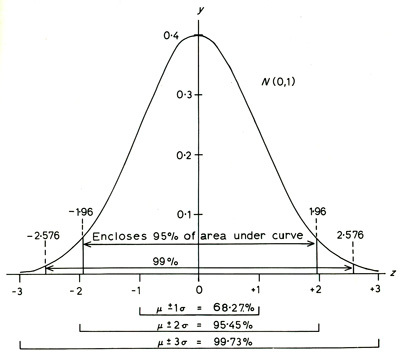
\includegraphics[width=5.56in]{images/gaussian-distribution} \caption{Standardoitu normaalijakauma: Virhemarginaaleja}\label{fig:unnamed-chunk-9}
\end{figure}

\
\
\
\

__Normaalijakauman odotusarvon luottamusväli ($\sigma^2$ tuntematon)__

- Tarkastellaan edelleen satunnaisotosta normaalijakaumasta, mutta oletetaan nyt että varianssi $\sigma^2$ tuntematon.

- Normaalijakauman odotusarvon $(1-\alpha) \times 100$\% luottamusväli:
$$
\Big(\bar{Y} - t_{\alpha/2} \frac{S}{\sqrt{n}}, 
\bar{Y} + t_{\alpha/2} \frac{S}{\sqrt{n}} \Big),
$$
jossa __luottamuskertoimet__ $-t_{\alpha/2}$ ja $t_{\alpha/2}$
saadaan nyt __$t$-jakaumasta} $t_{n-1}$, jossa $S^2$ on varianssin $\sigma^2$ harhaton estimaattori ja vapausasteiden lukumäärä on $n-1$.

  - (Studentin) $t$-jakauma muistuttaa silmämääräisesti normaalijakaumaa, mutta se on paksuhäntäisempi. Vapausasteluvun kasvaesssa $t$-jakauma lähestyy normaalijakaumaa.

  - Suurissa otoksissa ($n$ iso) luottamuskertoimet voidaan poimia (approksimatiivisesti) myös normaalijakaumasta eli korvata edellä kertoimet $t_{\alpha/2}$ aiemmin käytetyillä kertoimilla $z_{\alpha/2}$.

  - Normaalijakauman odotusarvon luottamusväli ($\sigma^2$ tuntematon), $t$-jakauma eri vapausastein $df$

\begin{figure}
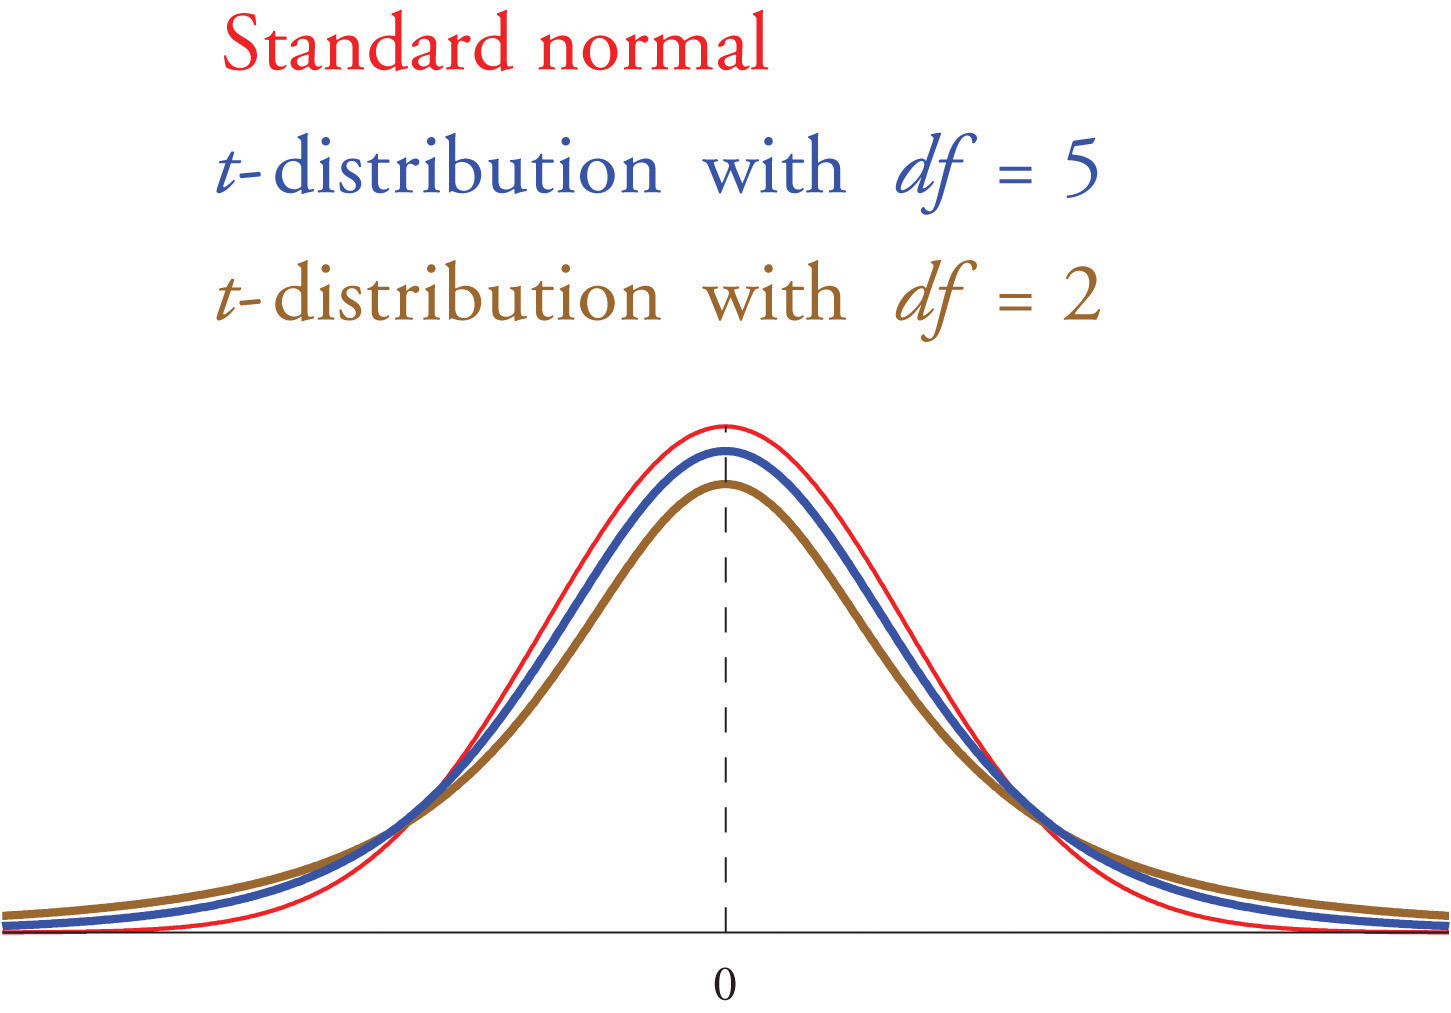
\includegraphics[width=20.15in]{images/NjaT-jakauma} \caption{Standardoitu normaalijakauma: Virhemarginaaleja}\label{fig:unnamed-chunk-10}
\end{figure}

\
\
\
\

__Luottamusväli: Suhteellisen osuuden odotusarvo__

- Käsittelemme seuraavassa suhteellisen osuuden $p$ luottamusvälejä.

- Tarkastellaan satunnaisotosta Bernoulli-jakaumasta 
$Y_1, \ldots, Y_n \indep, \,\, Y_i \thicksim B(p),\, i=1,\ldots,n$,
jossa merkitään $Y_i=1$ jos tapahtuma A tapahtuu ja $Y_i=0$ jos tapahtuma A ei tapahdu.

- Bernoulli-jakauman odotusarvoparametrin $p=\text{E}(Y_i)$ harhaton estimaattori on tapahtuman A suhteellinen otosfrekvenssi
$$
\widehat{p} = \frac{1}{n} \sum_{i=1}^{n} Y_i.
$$

- Bernoulli-jakauman (vrt. binomijakauma) ominaisuuksien 
perusteella $\text{E}(Y_i)=p$ ja $\mathrm{Var}(Y_i)=pq$, jossa
$q=1-p$.

- Näin ollen voimme normaalijakauman odotusarvoparametrin
luottamusvälin konstruloinnin tapaan määritellä satunnaismuuttujan $Z$:
$$
Z = \frac{\widehat{p} - p}{\sqrt{\frac{p (1-p)}{n}}} = 
\sqrt{n} \Big(\frac{\widehat{p} - p}{\sqrt{p (1-p)}} \Big),  
$$
joka noudattaa (suurissa otoksissa) $\text{N}(0,1)$-jakaumaa.

- Suhteellisen frekvenssin hajonnan estimaattori on siis
$$
\sqrt{\frac{\widehat{p} (1-\widehat{p})}{n}},
$$
jossa tuntematon $p$ on korvattu sen estimaattorilla (otosvastineella) $\widehat{p}$.


- Luottamuskertoimet määrätään aiempaan tapaan:
$$
\text{P}(-z_{\alpha/2} \le Z \le z_{\alpha/2}) = 1-\alpha,
$$


- Näin ollen odotusarvoparametrin (suhteellisen osuuden) $p$ $(1-\alpha)$% luottamusväliksi
saadaan
$$
\Big(
\widehat{p} - z_{\alpha/2} \sqrt{\frac{\widehat{p}(1-\widehat{p})}{n}},
\widehat{p} + z_{\alpha/2} \sqrt{\frac{\widehat{p}(1-\widehat{p})}{n}} 
\Big)
$$

- Luottamusväli voidaan kirjoittaa
$$
\widehat{p} \pm z_{\alpha/2} \sqrt{\frac{\widehat{p}(1-\widehat{p})}{n}}
$$
ja luottamusvälin pituus on 
$$
2 \times z_{\alpha/2} \sqrt{\frac{\widehat{p}(1-\widehat{p})}{n}}.
$$

## Otoskoko {#alaluku67}


<!--chapter:end:06-tilppa.Rmd-->

# Tilastollinen riippuvuus ja korrelaatio {#luku7}

- Tarkastelemme tässä luvussa tilastollisia tutkimusasetelmia, joissa on mukana kaksi tai useampia __muuttujia__. 

- Pyrimme vastaamaan tässä ja seuraavissa luvuissa (ainakin) seuraaviin kysymyksiin:

  - Miten kahden (tai useamman) muuttujan samanaikainen tarkastelu vaikuttaa tilastolliseen analyysiin?
  - Mitä tarkoitetaan kahden muuttujan tilastollisella riippuvuudella ja miten se eroaa eksaktista riippuvuudesta?
  - Mitä tarkoitetaan korrelaatiolla?
  - Mikä on korrelaation ja riippuvuuden suhde?
  - Miten korrelaatiota ja sen voimakkuutta voidaan estimoida?

- Käsittelemme myös jatkossa regressioanalyysia yhden selittäjän lineaarisen regressiomallin tapauksessa. Pitemmälle meneviä regressioanalyysin kysymyksiä käsitellään koko tilastotieteen opinto-ohjelman lävitse, kuten perusteellisesti Lineaariset ja yleistetyt lineaariset mallit -kurssin myötä.

## Muuttujien väliset riippuvuudet tilastollisen tutkimuksen kohteena {#alaluku71}

- Tieteellisen tutkimuksen tärkeimmät ja mielenkiintoisimmat kysymykset liittyvät tavallisesti __tutkimuksen kohteena olevaa ilmiötä kuvaavien muuttujien välisiin riippuvuuksiin__.

- Jos tilastollisen tutkimuksen kohteena olevaan ilmiöön liittyy useampia kuin yksi muuttuja, yhden muuttujan tilastolliset menetelmät antavat tavallisesti vain rajoittuneen kuvan ilmiöstä.

- Sovellusten kannalta ehkä merkittävin osa tilastotiedettä käsittelee kahden tai useamman muuttujan välisten riippuvuuksien kuvaamista ja mallintamista.

::: {.eblock .kimmo data-latex="{}"}
**Esimerkkejä riippuvuustarkasteluista**  

- Miten työttömyysaste Suomessa (% työvoimasta) riippuu BKT:n (bruttokansantuotteen) kasvuvauhdista Suomessa, Suomen viennin volyymista sekä BKT:n kasvuvauhdista muissa EU-maissa ja USA:ssa? Taloustieteilijät pyrkivät yleisesti löytämään muitakin lainalaisuuksia. Esimerkkejä tällaisista ovat riskin ja tuoton välinen suhde osakesijoittamisessa, hajauttaminen pienentää riskiä ja/tai alhainen korkotaso suosii sijoittamista pörssiin.  
- Miten alkoholin kulutus (l per capita vuodessa) riippuu alkoholijuomien hintatasosta, ihmisten käytettävissä olevista tuloista ja alkoholin saatavuudesta?  
- Miten todennäköisyys sairastua keuhkosyöpään riippuu tupakoinnin määrästä ja kestosta?  
- Miten vehnän hehtaarisato (t/ha) riippuu kesän keskilämpötilasta ja sademäärästä sekä maan muokkauksesta, lannoituksesta ja tuholaisten torjunnasta?  
- Miten betonin lujuus (kg/cm2)  riippuu sen kuivumisajasta?  
- Miten kemiallisen aineen saanto (%) riippuu valmistusprosessissa käytettävästä lämpötilasta? 
:::

\
\

- __Eksakti__ vs. __tilastollinen riippuvuus__
  - Tarkastelemme tässä esityksessä yksinkertaisuuden vuoksi pääasiassa kahden muuttujan välistä riippuvuutta:
    - (i) Muuttujien välinen riippuvuus on __eksaktia__, jos toisen arvot voidaan ennustaa tarkasti toisen saamien arvojen perusteella.
    - (ii) Muuttujien välinen riippuvuus on __tilastollista__, jos niiden välillä ei ole eksaktia riippuvuutta, mutta toisen muuttujan arvoja voidaan käyttää apuna toisen muuttujan arvojen ennustamisessa.

- Tilastollinen riippuvuus ja __korrelaatio__
  - Kahden muuttujan välistä (lineaarista) tilastollista riippuvuutta kutsutaan tilastotieteessä (tavallisesti) __korrelaatioksi__.
  - Korrelaation eli (lineaarisen) tilastollisen riippuvuuden voimakkuutta mittaavia tilastollisia tunnuslukuja kutsutaan korrelaatiokertoimiksi.
  - Korrelaatiot muodostavat perustan muuttujien välisten riippuvuuksien ymmärtämiselle.
  - Vaikka korrelaatiot muodostavat perustan muuttujien välisten riippuvuuksien ymmärtämiselle, riippuvuuksia halutaan tavallisesti analysoida myös tarkemmin.
  - __Regressioanalyysi__ on tilastollinen menetelmä, jossa jonkin, ns. selitettävän muuttujan tilastollista riippuvuutta joistakin toisista, ns. selittävistä muuttujista pyritään mallintamaan regressiomalliksi kutsutulla tilastollisella mallilla. Käsittelemme johdatusta regressioanalyysin vielä myöhemmin luvussa \\ref{luku8}.

## Kahden muuttujan havaintoaineiston kuvaaminen {#alaluku72}

- Kuten yhden muuttujan havaintoaineistojen tapauksessa, lähtökohdan kahden tai useamman muuttujan havaintoaineistojen kuvaamiselle muodostaa tutustuminen havaintoarvojen jakaumaan.

- Havaintoarvojen jakaumaa voidaan kuvailla ja esitellä tiivistämällä havaintoarvoihin sisältyvä informaatio sopivaan muotoon:
  - Havaintoarvojen jakaumaa kokonaisuutena voidaan kuvata sopivasti valituilla graafisilla esityksillä.
  - Havaintoarvojen jakauman karakteristisia ominaisuuksia voidaan kuvata sopivasti valituilla otostunnusluvuilla (ks. otostunnuslukuja ja otosjakaumat luvussa \\ref{luku6} ).

- Koska useampi- kuin kaksiulotteisten kuvioiden tekeminen ei ole usein kovin mielekästä, kolmen tai useamman muuttujan havaintoaineistoja havainnollistetaan tavallisesti niin, että muuttujia tarkastellaan pareittain.

- Kahden järjestys-, välimatka- tai suhdeasteikoillisen muuttujan havaittujen arvojen pareja havainnollistetaan tavallisesti graafisella esityksellä, jota kutsutaan hajontakuvioksi tai pistediagrammiksi ("pistekaavio" engl. scatter plot).

- Usean muuttujan havaintoaineistojen karakteristisia ominaisuuksia voidaan kuvata muuttujakohtaisilla otostunnusluvuilla.

- Muuttujakohtaiset otostunnusluvut eivät kuitenkaan voi antaa informaatiota muuttujien välisistä riippuvuuksista.

- Muuttujien pareittaisia tilastollisia riippuvuuksia voidaan kuvata sopivasti valitulla korrelaation mitalla.

\
\

__Pistediagrammi (hajontakuvio)__

- Tarkastellaan tilannetta, jossa tutkimuksen kohteina olevista havaintoyksiköistä on mitattu kahden järjestys-, välimatka- tai suhdeasteikollisen muuttujan $X$ ja $Y$ arvot.

- Muuttujien $X$ ja $Y$ arvojen samaan havaintoyksikköön liittyvien parien $(X,Y)$ muodostamaa havaintoaineistoa voidaan kuvata graafisesti pistediagrammilla.

- Pistediagrammi sopii erityisesti kahden muuttujan välisen riippuvuuden havainnollistamiseen. Se on keskeinen työväline korrelaatio- ja regressioanalyysissa.

::: {.noteblock .mikko data-latex="{}"}
**Pistediagrammi**  

Olkoot $X$ ja $Y$ järjestys-, välimatka- tai suhdeasteikollisia muuttujia, joiden havaitut arvot ovat $x_1, x_2, \ldots, x_n$ ja $y_1, y_2, \ldots, y_n$. Oletetaan lisäksi, että havaintoarvot $x_i$ ja $y_i$ liittyvät samaan havaintoyksikköön kaikille $i = 1, 2, \ldots, n$. Havaintoarvojen parien $(x_i, y_i)$ pistediagrammi saadaan esittämällä lukuparit niiden määrittelemien pisteiden tasokoordinaatistossa.
:::

\
\

::: {.eblock .kimmo data-latex="{}"}
**Esimerkki: Isän ja pojan pituus**  

- Perinnöllisyystieteen mukaan lapset perivät geneettiset ominaisuutensa vanhemmiltaan.
- Periytyykö isän pituus heidän pojilleen?
- Havaintoaineisto koostuu 300:n isän ja heidän poikiensa pituuksien muodostamasta lukuparista $(x_i , y_i),\, i = 1, 2, \ldots, 300$, jossa $x_i$ = isän $i$ pituus ja $y_i$ = isän $i$ pojan pituus.
- Yhtä pitkillä isillä näyttää olevan monen mittaisia poikia.
- Mutta: Lyhyillä isillä näyttää olevan keskimäärin lyhyempiä poikia kuin pitkillä isillä ja pitkillä isillä näyttää olevan keskimäärin pitempiä poikia kuin lyhyillä isillä.
- Tällaisten tilastollisten riippuvuuksien analysoimista lineaaristen regressiomallien avulla tarkastellaan myöhemmin luvussa \\ref{luku8} Yksinkertainen lineaarinen regressiomalli. 
:::

\begin{figure}
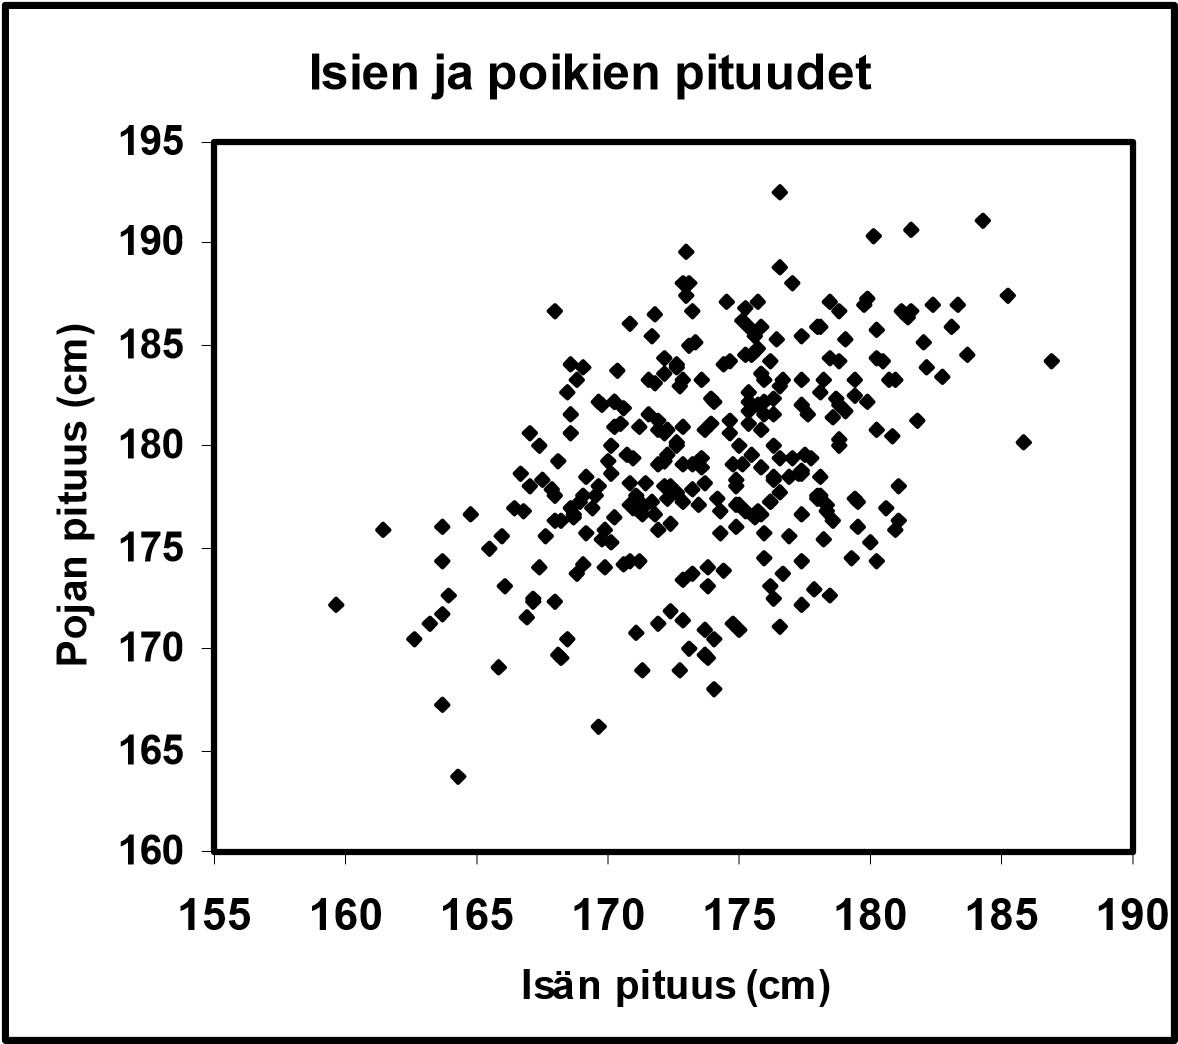
\includegraphics[width=16.36in]{images/Isien-poikien-pituudet-Mellin} \caption{Isien ja poikien pituudet. Lähde: Mellin (2006).}\label{fig:unnamed-chunk-11}
\end{figure}

## Tunnusluvut {#alaluku73}

- Kahden välimatka- tai suhdeasteikollisen muuttujan havaintoarvojen parien muodostamaa jakaumaa voidaan karakterisoida seuraavilla tunnusluvuilla:
  - Havaintoarvojen keskimääräistä sijaintia kuvataan aritmeettisilla keskiarvoilla.
  - Havaintoarvojen hajaantuneisuutta tai keskittyneisyyttä kuvataan keskihajonnoilla tai (otos-) variansseilla.
  - Havaintoarvojen (lineaarista) riippuvuutta kuvataan otoskovarianssilla ja otoskorrelaatiokertoimella.

- Ts. oletetaan seuraavassa, että meillä on käytettävissä välimatka- tai suhdeasteikollisten muuttujien x ja y havaittuja arvoja $x_1, x_2, \ldots, x_n$ ja $y_1, y_2, \ldots, y_n$. Oletetaan lisäksi, että havaintoarvot $x_i$ ja $y_i$ liittyvät samaan havaintoyksikköön kaikille $i = 1, 2, \ldots, n$. Havaintoarvojen parien $(x_i, y_i)$

- Käsitellään seuraavassa otoskeskiarvoa ja otosvarianssia. Olemme käsitelleet vastaavia estimaattoreita jo aiemmin luvussa \\ref{luku6}.

- Havaintoarvojen $y_1, y_2,\ldots, y_n$ aritmeettinen keskiarvo on
$$
    \bar{y} = \frac{1}{n} \sum_{i=1}^{n} y_i.
$$
Vastaavalla tavalla voidaan määritellä havaintojen $x_1, x_2, \ldots, x_n$ (aritmeettinen) keskiarvo $\bar{x}=\frac{1}{n}\sum_{i=1}^{n}x_i$.
  - Havaintoarvojen pareista $(x_i, y_i ), \, i = 1, 2,\ldots,n$ laskettujen aritmeettisten keskiarvojen, otoskeskiarvojen, $\bar{x}$ ka $\bar{y}$ muodostama lukupari ($\bar{x}, \bar{y})$ on havaintoarvojen parien muodostamien pisteiden painopiste.
  - Havaintoarvojen aritmeettinen keskiarvo kuvaa havaintoarvojen keskimääräistä sijaintia.
  - Osoittautuu, että (aritmeettinen) keskiarvo toimii tilastollisessa mielessä hyvänä estimaattorina satunnaismuuttujan $y$ odotusarvolle. 

\
\

__Otosvarianssi__: Havaintoarvojen $y_1, y_2,\ldots, y_n$ (otos-) varianssi (on todettu jo aiemmin) on muotoa
$$
    S^2_y = \frac{1}{n-1} \sum_{i=1}^{n} (y_i - \bar{y})^2,
$$
jossa $\bar{y}$ on on y-havaintoarvojen aritmeettinen keskiarvo. 
  - Jälleen vastaavalla tavalla voidaan määritellä x-havaintoarvojen (otos-) varianssi $S^2_x$.
  - Havaintoarvojen varianssi mittaa havaintoarvojen hajaantuneisuutta tai keskittyneisyyttä havaintoarvojen aritmeettisen keskiarvon suhteen.
    
- __(Otos-) keskihajonta__: Havaintoarvojen $y_1, y_2,\ldots, y_n$ (otos-) keskihajonta
$$
    s_y = \sqrt{s^2_y} = \sqrt{\frac{1}{n-1} \sum_{i=1}^{n} (y_i - \bar{y})^2},
$$
jossa $\bar{y}$ on on y-havaintoarvojen aritmeettinen keskiarvo. Huomaa suhde (otosvarianssiin.
  - Jälleen vastaavalla tavalla voidaan määritellä x-havaintoarvojen (otos-) keskihajonta $s_x$.
  - Havaintoarvojen keskihajonta mittaa havaintoarvojen hajaantuneisuutta tai keskittyneisyyttä havaintoarvojen aritmeettisen keskiarvon suhteen.

\
\

## Satunnaismuuttujien kovarianssi ja korrelaatio {#alaluku74}

- Tarkastellaan välimatka- tai suhdeasteikollisten satunnaismuuttujien $X$ ja $Y$ Pearsonin (tulomomentti-) korrelaatiokerrointa $\rho_{XY}$ ja sen estimointia.

- Tällä kurssilla emme tarkastele tarkemmin tilastollisia testejä korrelaatiokertoimelle $\rho_{XY}$, kuten:
  -Yhden otoksen testi korrelaatiokertoimelle
  -Korrelaatiokertoimien vertailutesti
  -Korreloimattomuuden testaaminen

- Jälleen kerran, lisätietoja ja tarkempia yksityiskohtia moniulotteisista satunnaismuuttujista ja jakaumista tarkastellaan todennäköisyyslaskennan kursseilla.

::: {.noteblock .miko data-latex="{}"}
**Satunnaismuuttujien kovarianssi ja korrelaatio**  

 Olkoon $(X, Y)$ satunnaismuuttujien $X$ ja $Y$ muodostama järjestetty pari. Olkoot 
$$
    \mu_X = \text{E}(X) \qquad \mathrm{and} \qquad  \mu_Y = \text{E}(Y)
$$
satunnaismuuttujien $X$ ja $Y$ odotusarvot ja
$$
   \sigma^2_X = \mathrm{Var}(X) = \text{D}^2(X) = \text{E}[(X- \mu_X)^2] \\
   \sigma^2_Y = \mathrm{Var}(Y) = \text{D}^2(Y) = \text{E}[(Y- \mu_Y)^2]
$$
satunnaismuuttujien $X$ ja $Y$ varianssit. 
\

Määritellään satunnaismuuttujien $X$ ja $Y$ kovarianssi $\sigma_{XY}$ kaavalla
$$
\sigma_{XY} = \mathrm{Cov}(X,Y) = \text{E}[(X-\mu_X)(Y-\mu_Y)]
$$

Määritellään satunnaismuuttujien $X$ ja $Y$ korrelaatio $\rho_{XY}$ kaavalla
$$
\rho_{XY} = \mathrm{Cor}(X,Y) = \frac{\sigma_{XY}}{\sigma_{X} \sigma_{Y}},
$$
jossa siis $\sigma_X = \sqrt{\mathrm{Var}(X)} = \sqrt{\text{D}^2(X)}$ ja $\sigma_Y = \sqrt{\mathrm{Var}(Y)} = \sqrt{\text{D}^2(Y)}$
:::

- Satunnaismuuttujien $X$ ja $Y$ korrelaatiota
$$
\rho_{XY} = \mathrm{Cor}(X, Y)
$$
kutsutaan ajoittain __Pearsonin korrelaatiokertoimeksi__ (tulomomenttikorrelaatiokertoimeksi).
  - Pearsonin korrelaatiokerroin $\rho_{XY}$ mittaa satunnaismuuttujien $X$ ja $Y$ lineaarisen riippuvuuden voimakkuutta. Ts. sm:jien välistä (lineaarista) yhteyttä.

- Pearsonin (tulomomentti-) korrelaatiokerroin voidaan estimoida vastaavalla Pearsonin __otoskorrelaatiokertoimella__ 
$$
r_{XY} = \frac{s_{XY}}{s_X s_Y}
$$
Estimaattori $r_{XY}$ voidaan johtaa sekä momenttimenetelmällä että suurimman uskottavuuden menetelmällä, jotka ovat tyypillisiä estimointimenetelmiä tilastotieteessä ja tarkemmin tilastollisessa päättelyssä.

::: {.noteblock .miko data-latex="{}"}
**Pearsonin otoskorrelaatiokerroin**

Havaintoarvojen $(x_i, y_i)$ pareista laskettu __otoskovarianssi__ on
$$
s_{xy} = \frac{1}{n-1} \sum_{i=1}^{n} (x_i - \bar{x}) (y_i - \bar{y}),
$$
jossa $\bar{x}$ ja $\bar{y}$ ovat havaintoarvojen $x$ ja $y$ aritmeettiset keskiarvot.
\
Otoskovarianssin $s_{xy}$ avulla voidaan määritellä $x$- ja $y$-havaintoarvojen lineaarisen tilastollisen riippuvuuden voimakkuuden mittari, jota kutsutaan Pearsonin otoskorrelaatiokertoimeksi. Pearsonin otoskorrelaatiokerroin $r_{xy}$ saadaan otoskovarianssista $s_{xy}$ __normeerausoperaatiolla__, jossa otoskovarianssi $s_{xy}$ jaetaan $x$- ja $y$-havaintoarvojen keskihajonnoilla $s_x$ ja $s_y$. 
\
Ts. havaintoarvojen pareista $(x_i, y_i), i = 1, 2, \ldots, n$ laskettu Pearsonin otoskorrelaatiokerroin on siis
$$
r_{xy} = \frac{s_{xy}}{s_x s_y} = \frac{\sum_{i=1}^{n} (x_i - \bar{x}) (y_i - \bar{y})}{\sqrt{\sum_{i=1}^{n} (x_i - \bar{x})^2} \sqrt{\sum_{i=1}^{n} (y_i - \bar{y})^2}} , 
$$
jossa $s_{xy}$ on $x$- ja $y$-havaintoarvojen otoskovarianssi, $s_x$ on $x$-havaintoarvojen keskihajonta ja $s_y$ on y-havaintoarvojen keskihajonta.
:::

- Otoskovarianssi:
  - Huomaa, että $x$- ja $y$-havaintoarvojen otoskovarianssit niiden itsensä kanssa ovat niiden variansseja.
  - Otoskovarianssi $s_{xy}$ mittaa $x$- ja $y$-havaintoarvojen yhteisvaihtelua niiden aritmeettisten keskiarvojen ympärillä.
  - Otoskovarianssilla on taipumus saada positiivisia (negatiivisia) arvoja, jos havaintopisteiden muodostama "pistepilvi (pisteparvi)" näyttää nousevalta (laskevalta) oikealle mentäessä; ks. pistediagrammin ilmeen ja Pearsonin otoskorrelaatiokertoimen yhteys, jota käsitellään seuraavaksi.

- Pearsonin otoskorrelaatiokertoimella $r_{xy}$ on seuraavat ominaisuudet:
  - (i) $-1 \le r_{xy} \le 1$
  - (ii) $r_{xy} = \pm 1$, jos ja vain jos $y_i = \alpha \beta x_i$, jossa $\alpha$ ja $\beta$  ovat reaalisia vakiota ja $\beta \neq 0$
  - (iii)   Korrelaatiokertoimella $r_{xy}$ ja kovarianssilla $s_{xy}$ on aina sama etumerkki

- Pearsonin otoskorrelaatiokerroin $r_{xy}$: Tulkinta/tulkintoja:
  - Havaintoarvojen pareista $(x_i, y_i), i = 1,2, \ldots, n$ laskettu Pearsonin otoskorrelaatiokerroin $r_{xy}$ mittaa $x$- ja $y$-havaintoarvojen lineaarisen tilastollisen riippuvuuden voimakkuutta.
  - Jos $r_{xy} = \pm 1$, niin $x$- ja $y$-havaintoarvojen välillä on eksakti eli funktionaalinen lineaarinen riippuvuus, mikä merkitsee sitä, että kaikki havaintopisteet $(x_i, y_i)$ asettuvat samalle suoralle.
  - Jos $r_{xy} = 0$, niin $x$- ja $y$-havaintoarvojen välillä ei voi olla eksaktia lineaarista riippuvuutta.
  - Vaikka $r_{xy} = 0$, $x$- ja $y$-havaintoarvojen välillä saattaa silti olla jopa eksakti epälineaarinen riippuvuus.

- __Havainnollistus__: Kuviot alla havainnollistavat kahden muuttujan havaittujen arvojen ($n = 30$) pistediagrammin ilmeen ja korrelaation välistä yhteyttä.

\begin{figure}
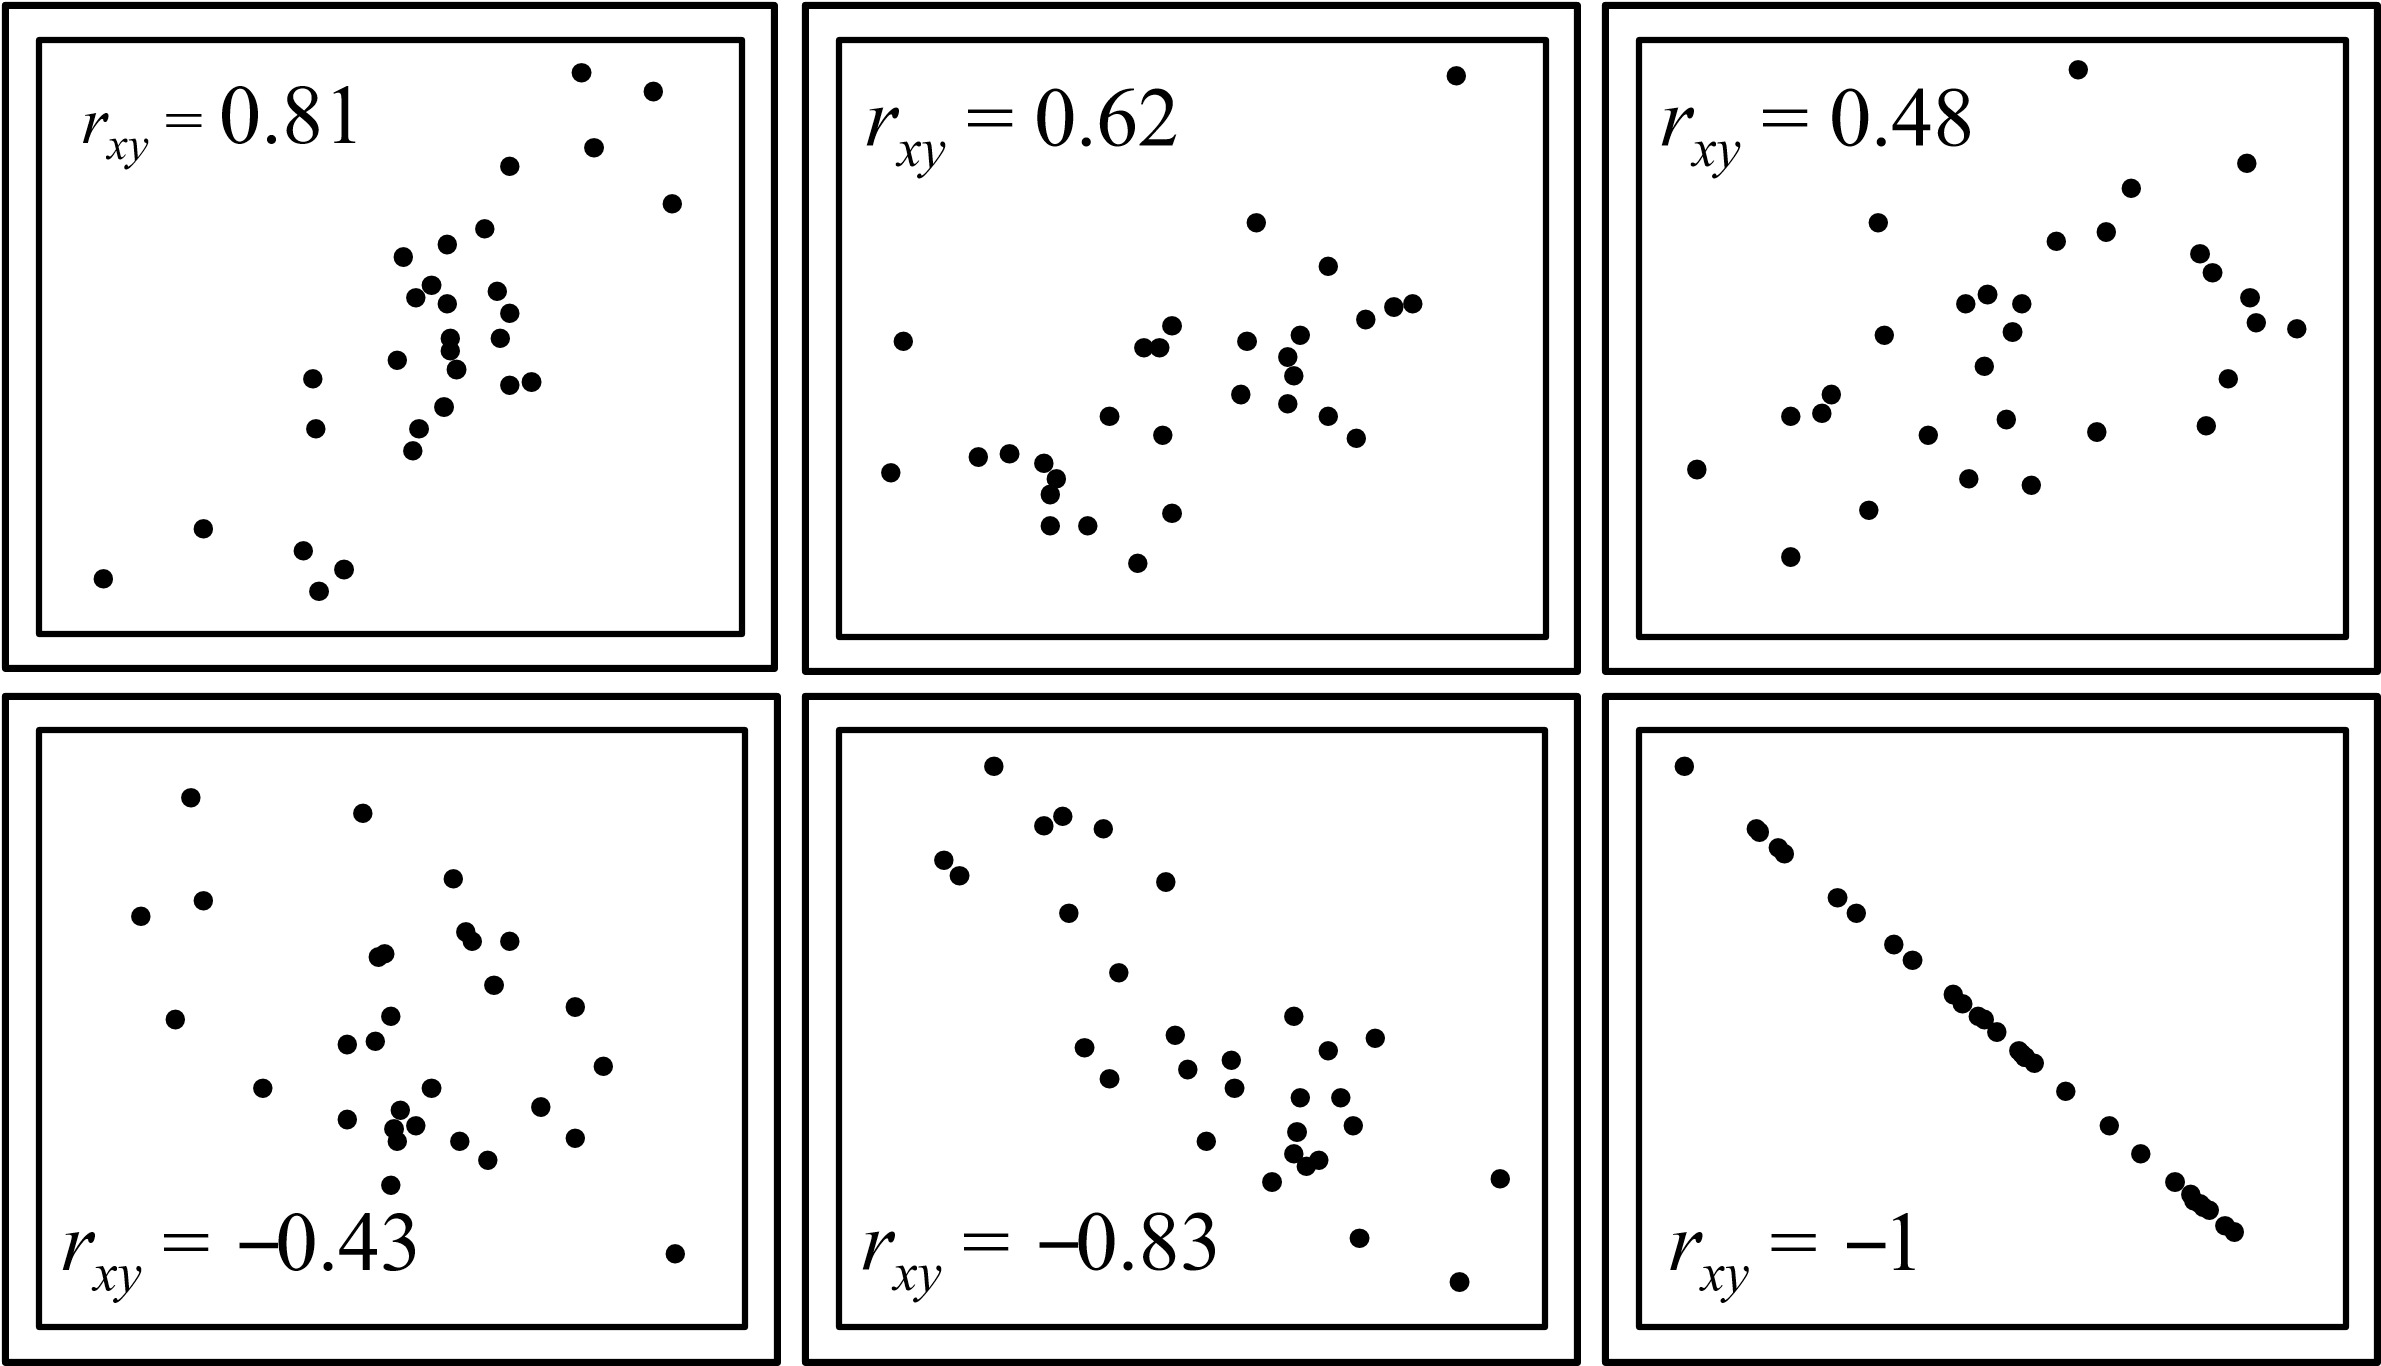
\includegraphics[width=33.07in]{images/Pearson-korr-Mellin} \caption{Havainnollistuksia Pearsonin otoskorrelaatiokertoimen arvosta ja erilaisista $xy$-pisteparvista. Lähde: Mellin (2006).}\label{fig:unnamed-chunk-12}
\end{figure}

- Toinen havainnollistus: Ks. seuraavasta linkistä lisää havainnollistuksia. Arvio korrelaation voimakkuutta erilaisissa simuloiduissa tilanteissa: \url{}


```
## PhantomJS not found. You can install it with webshot::install_phantomjs(). If it is installed, please make sure the phantomjs executable can be found via the PATH variable.
```

<iframe src="http://guessthecorrelation.com/" width="100%" height="400px" data-external="1"></iframe>

\
\

- __Kausaalisuus__
  - Muuttujan $x$ arvojen muutos vaikuttaaa muuttujan $y$ arvoihin (syy-vaikutussuhde), jos seuraavat kolme ehtoa täyttyvät:
    - muuttujan $x$ muutos esiintyy ajallisesti ennen y:n muutosta
    - muuttujissa $x$ ja $y$ tapahtuvien muuttujien välillä on riippuvuutta
    - muuttujassa $y$ tapahtunutta muutosta ei voida selittää millään muilla tekjöillä

\begin{figure}
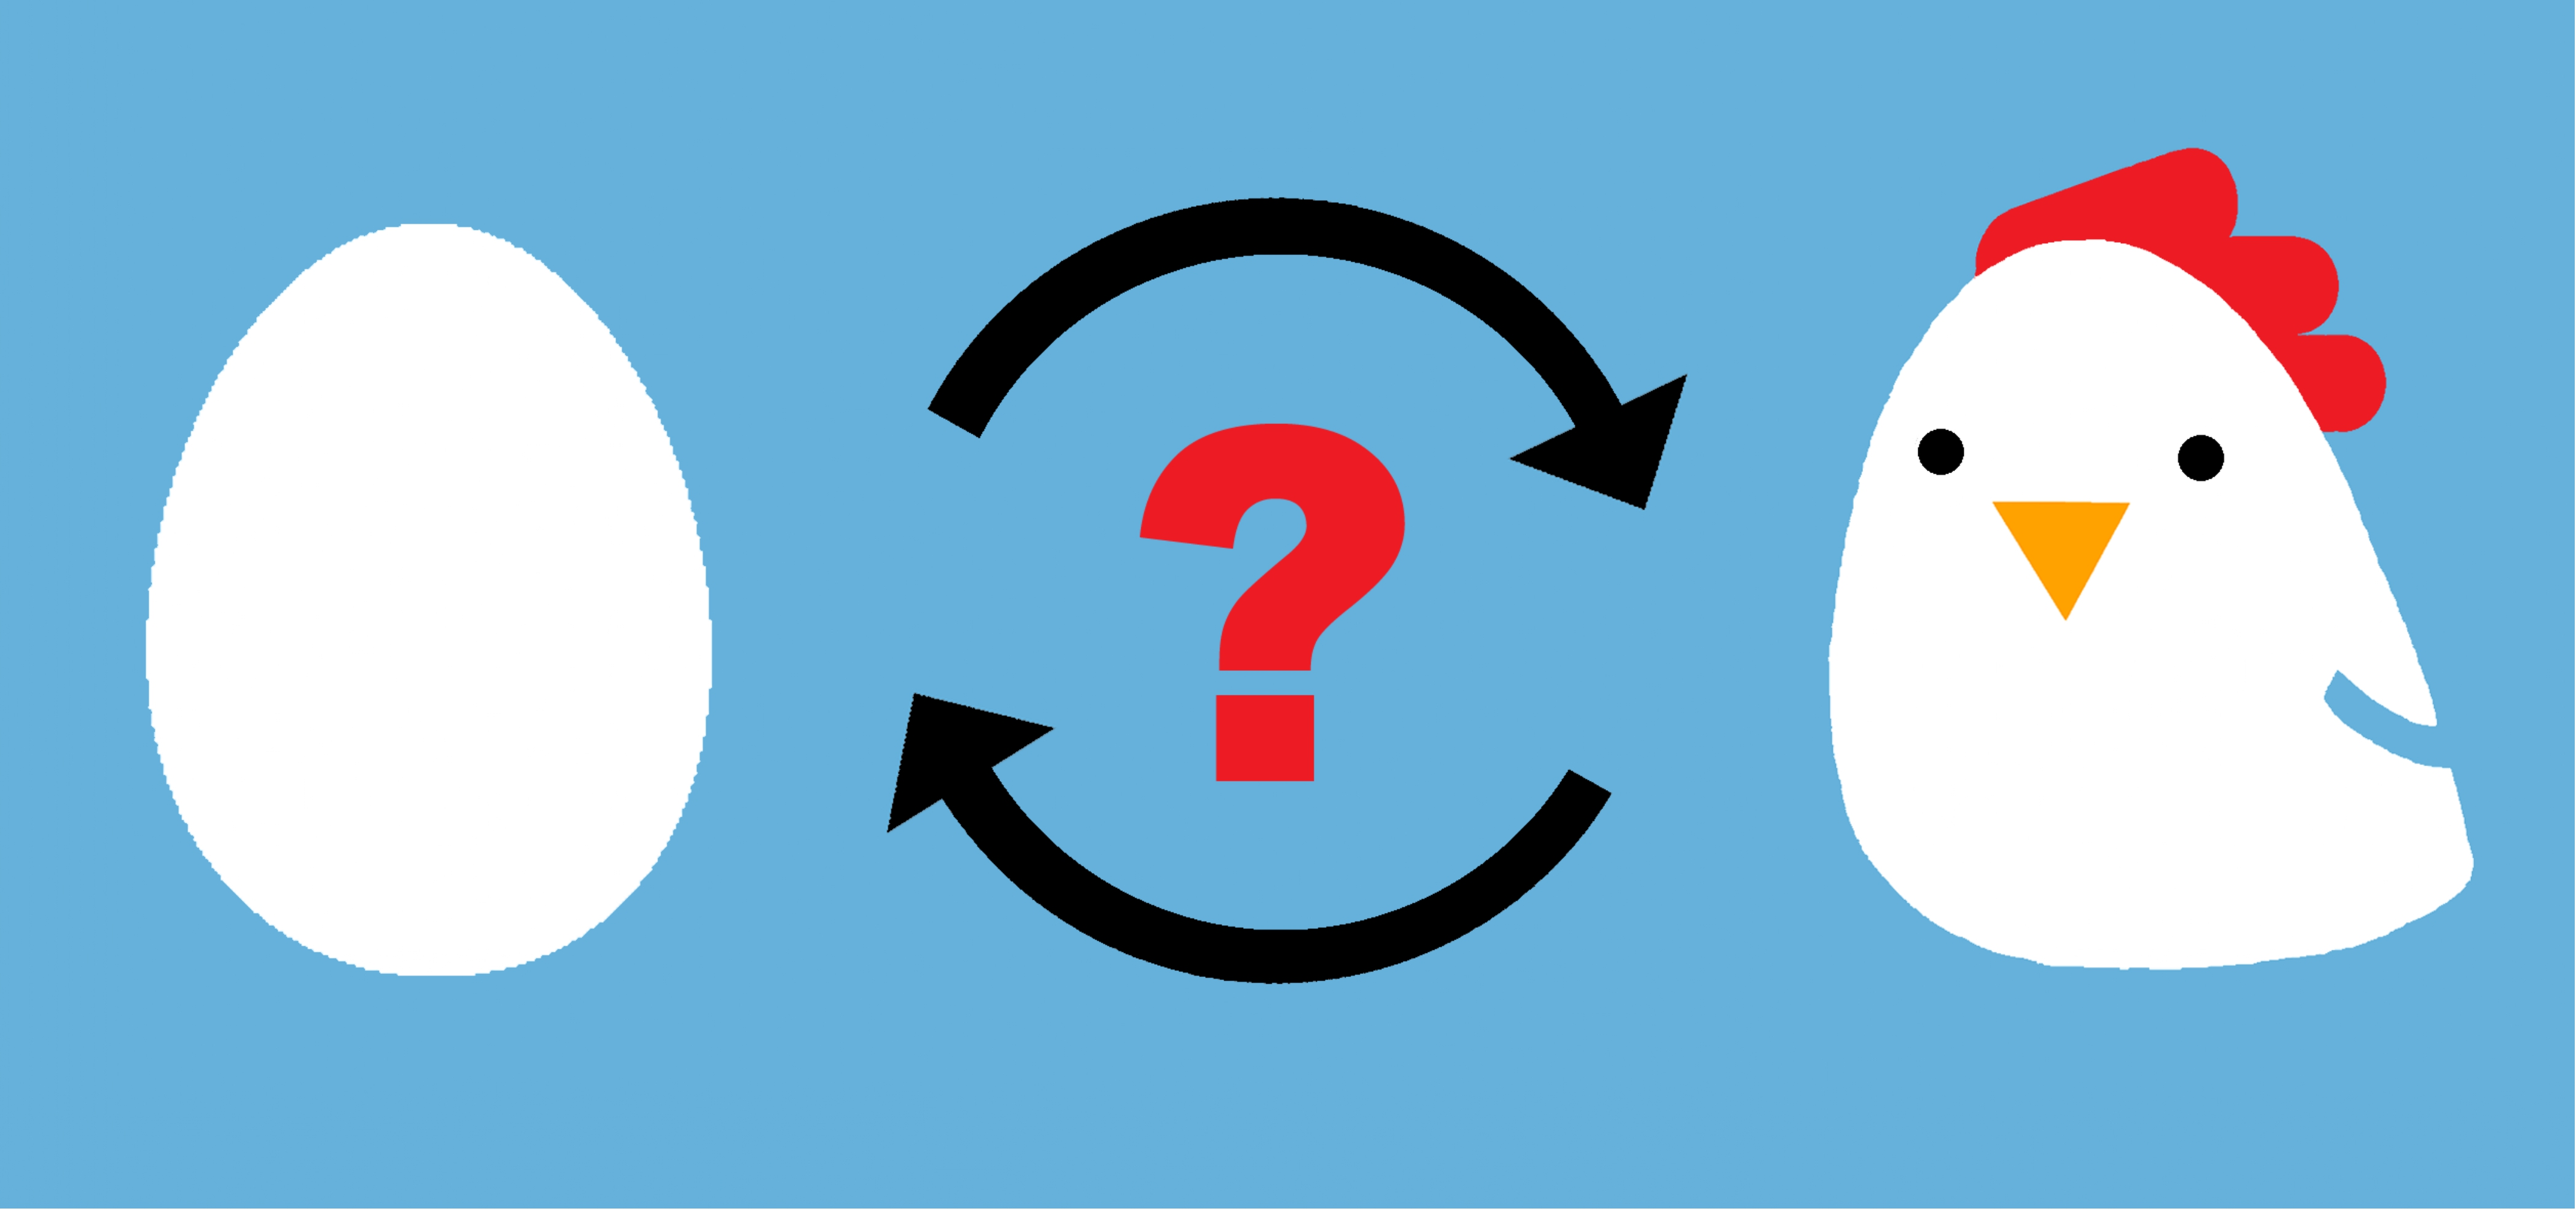
\includegraphics[width=58.25in]{images/causality} \end{figure}

- Kausaalisuhteita selvitettäessä on tunnettava etukäteen ilmiötä koskevat aiemmat teoriat ja tutkimukset tarkasti, jotta voidaan ottaa huomioon ilmiöön vaikuttavat tekijät

- Todellisuus on usein monimutkaisempi, kuin mitä kausaalisuhde kuvaa: __kahden muuttujan yhteisvaihtelu ei riitä todisteeksi siitä, että kyseessä olevien muuttujien välillä on kausaalista yhteyttä__

- Yhteisvaihtelu voi johtua myös kolmannen muuttujan vaikutuksesta molempiin muuttujiin tai virheellisestä otannasta, vaikka muuttujat olisivatkin perusjoukossa toisistaan riippumattomia

\begin{figure}
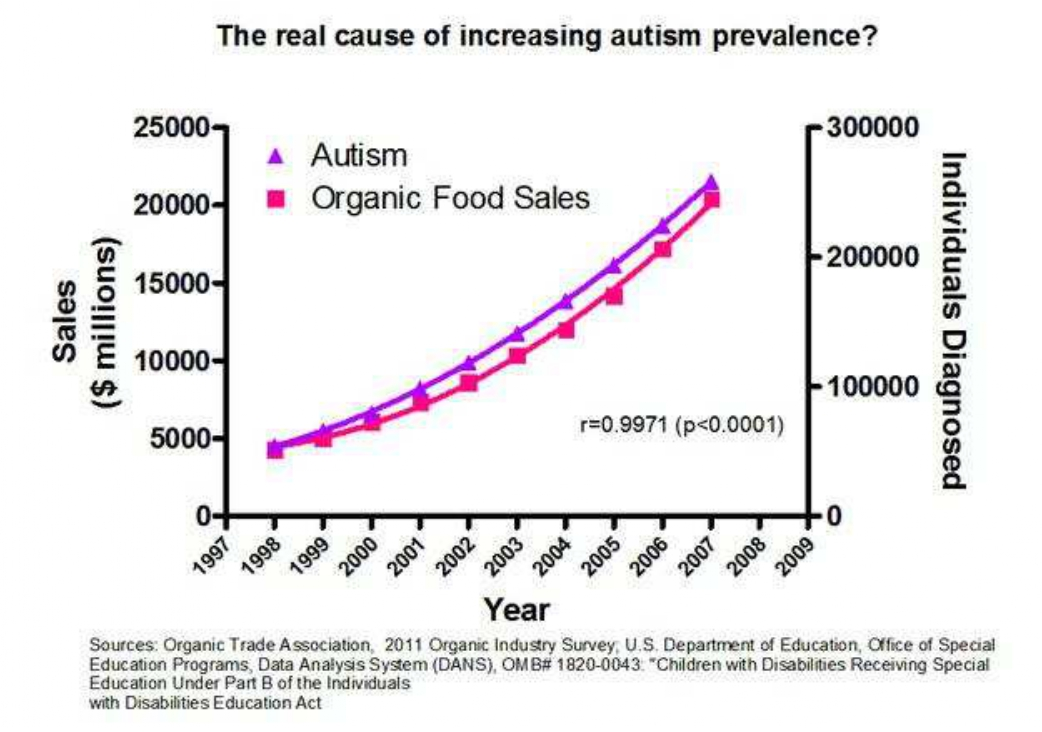
\includegraphics[width=14.47in]{images/causality2} \caption{Esimerkkejä: luomuruoka syypää lisääntyneisiin autismitapauksiin?}\label{fig:unnamed-chunk-15}
\end{figure}

- Simpsonin paradoksi
  - Simpsonin paradoksi syntyy, kun kahden muuttujan välinen korrelaatio muuttuu päinvastaiseksi, otettaessa huomioon jokin kolmas muuttuja, joka korreloi molempien muuttujien kanssa

\begin{figure}
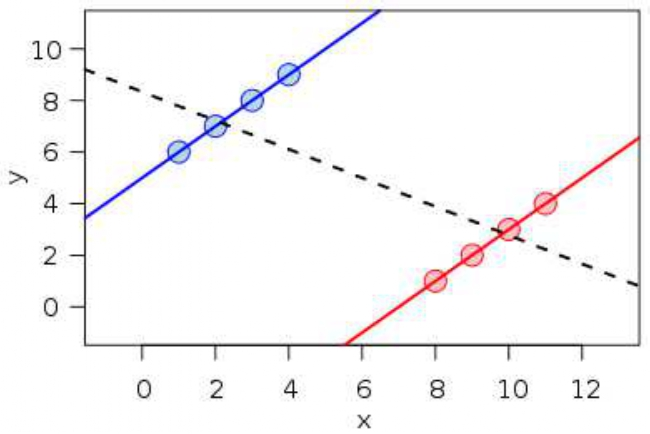
\includegraphics[width=9.03in]{images/simpson} \caption{Simpsonin paradoksi}\label{fig:unnamed-chunk-16}
\end{figure}

::: {.noteblock .mikko data-latex="{}"}
**Esimerkki: Berkeleyn sukupuolisyrjintä**

Yksi tunnetuimmista esimerkeistä Simpsonin paradoksista on Berkeleyn yliopiston sukupuolisyrjintätapaus. Yliopisto haastettiin oikeuteen vuonna 1973 sukupuolisyrjinnästä. Väitettiin, että yliopistoon olisi miesten helpompi päästä kuin naisten.
|  | Hakijat | Hyväksytyt |
|-----|-----|-----|
|Miehet|8442| __44%__ |
|Naiset|4321| 35% |
\
Taulukosta nähdään, että mieshakijoista on päässyt 9 prosenttiyksikköä enemmän sisälle kuin naisista.
\
\

- Tarkasteltaessa erikseen eri tiedekuntia huomataan, että itseasissa useammassa tiedekunnissa naisia on päässyt sisälle isompi osuus hakijoista. Aineisto kuudesta isoimmasta tiedekunnasta on listattu alla olevaan taulukkoon.
| | Miehet | | | Naiset | | |
|Tdk|Hakijat|Hyväksytyt|%|Hakijat|Hyväksytyt|%|
|--|--|--|--|--|--|--|
|A|825|62|108| __82__|
|B|560|63|25| __68__|
|C|325| __37__|593|34|
|D|417|33|375| __35__|
|E|191| __28__|393|24|
|F|373|6|341| __7__|
:::

\
\

- Vielä tiivistäen korrelaatiokertoimen tulkintavirheitä aiheuttavat useimmiten seuraavat seikat:
  - Riippuvuudesta ei välttämättä seuraa syy-seuraussuhdetta.
  - Kolmas muuttuja eli kahden muuttujan välinen yhteys selittyy yhteisestä syystä (esimerkiksi lämpimästä kesästä).
  - Muuttujien välinen yhteys ei ole lineaarinen.
  - Poikkeavien havaintojen vaikutus.
- Puutteita: Korrelaatiokertoimella on kaksi puutetta:
  - Se mittaa vain lineaarista riippuvutta.
  - Se ei ole (tilastollinen) malli, jonka avulla nähtäisiin, miten toinen muuttuja vaikuttaa toiseen muuttujaan. 

<!--chapter:end:07-korrelaatio.Rmd-->

# Regressioanalyysi {#luku8}

Tilastollinen riippuvuus ja korrelaatio -jakson laajennuksena pyrimme tässä luvussa vastaamaan seuraavaan kysymykseen: _Miten jonkin selitettävän muuttujan tilastollista riippuvuutta joistakin toisista, selittäviksi muuttujiksi kutsutuista muuttujista voidaan mallintaa_? Muuttujien välisten riippuvuuksien, eli erilaisten tosielämän asioiden ja ilmiöiden välisten yhteyksien analysointi on tavallisesti keskeinen kysymys tieteellisessä tutkimuksessa. Regressioanalyysi ja -mallintaminen on yksi tunnetuimpia ja eniten sovellettuja __tilastollisia menetelmiä__ kuvaamaan kahden muuttujan __tilastollista riippuvuutta__.

Jos tilastoaineistossa on havaittavissa säännönmukaisuutta ja muuttujien välillä näyttäisi olevan järkevä (asialooginen) yhteys, niin päästään "malliajatteluun". Ts. pyritään rakentamaan tilastollista mallia kys. aineistolle. Pyritään siis muodostaa tilastollinen malli että se valitun kriteeristön perusteella parhaiten kuvaa analysoitavaa pistejoukkoa.

## Johdatus regressioanalyysin ideaan {#alaluku81}

- Regressioanalyysi pyrkii siis havaintoaineiston perusteella __mallintamaan tilastoyksikköjen tilastollisten muuttujien välistä riippuvuutta__.
  - Regressiomallissa tilastollisia muuttujia on kahdenlaisia: __selitettävä muuttuja}, jonka tilastollista vaihtelua pyritään selittämään __selittävän muuttujan} vaihtelulla. 
  - Toisin sanoen, pyritään erottamaan se selitettävän muuttujan arvojen vaihtelu, joka voidaan selittää selittävän muuttujan arvojen vaihtelulla siitä vaihtelusta, joka on täysin satunnaista. 
    - Esimerkiksi voitaisiin tutkia selittääkö vaaleissa puolueiden/ehdokkaiden vaalimainontabudjetti heidän äänimääriään, ja jos, niin kuinka paljon? 
    - Jos __tilastollisesti merkitsevä osa__ selitettävän muuttujan havaittujen arvojen vaihtelusta voidaan selittää selittävien muuttujien arvojen vaihtelun avulla, sanomme, että selitettävä muuttuja __riippuu tilastollisesti__ selittäjinä käytetyistä muuttujista.

- Yleisemmin regressioanalyysi pyrkii vastaamaan seuraaviin kysymyksiin koskien tilastollisten muuttujien välistä riippuvuutta:
  - Muuttujien välisten __riippuvuuksien kuvaaminen__. Millainen on riippuvuuden muoto? Kuinka voimakasta riippuvuus on?
  - Muuttujien välisten __riippuvuuksien selittäminen__. Tilastollisen riippuvuuden luonteen selittäminen.
  - Selitettävän muuttujan käyttäytymisen __ennustaminen__.

- __Lineaarinen regressioanalyysi__ siis (teknisesti) rajoittuu muuttujien _lineaaristen_ riippuvuuksien kuvaamiseen. Kuitenkin, laajemmin asiaa pohdittaessa, lineaaristen regressiomallien suuri käyttökelpoisuus muuttujien välisten riippuvuuksien tilastollisessa analyysissa perustuu (ainakin) seuraaviin seikkoihin:
  - Lineaarisella regressiomallilla voidaan usein vähintään kohtuullisella (riittävällä) tarkkuudella approksimoida epälineaarisiakin muuttujien välisiä riippuvuuksia! 
  - Muuttujien välinen epälineaarinen riippuvuus voidaan usein myös linearisoida käyttäen sopivia muunnoksia alkuperäisiin muuttujiin.
  - Epälineaariset regressiomallit muodostavat oman tilastollisten (regressio)mallien luokkansa (joita ei käsitellä tällä kurssilla, mutta kylläkin myöhemmissä tilastotieteen opinnoissa).

\
\

- Regressiomalleja käytetään apuvälineinä monilla tilastotieteen osa-alueilla. Esimerkkejä regressiomallien käyttökohteista tilastotieteessä:
  - Varianssianalyysi
  - Koesuunnittelu
  - Monimuuttujamenetelmät
  - Biometria/biostatistiikka
  - Aikasarja-analyysi ja ennustaminen
  - Ekonometria

- Regressioanalyysissa sovellettavat tilastolliset mallit voidaan luokitella usealla eri periaatteella.
  - Luokittelu regressiomallin funktionaalisen muodon mukaan:
    - Lineaariset regressiomallit
    - Epälineaariset regressiomallit
  - Luokittelu regressiomallin yhtälöiden lukumäärän mukaan:
    - Yhden yhtälön regressiomallit
    - Moniyhtälömallit

Tällä kurssilla käsitellään vain __lineaarisia yhden yhtälön regressiomalleja__. Kuitenkin luvussa \\ref{alaluku83} [alapuolella] esitellään lyhyesti minkälaisia laajennuksia tälle regressioanalyysin perustilanteelle tyypillisesti käsitellään. 

## Yhden selittäjän lineaarinen regressiomalli {#alaluku82}

- Yhden selittäjän lineaarinen regressiomalli pyrkii selittämään selitettävän muuttujan havaittujen arvojen vaihtelun yhden selittävän muuttujan havaittujen arvojen vaihtelun avulla. Se on siis yksinkertaisin esimerkki yhden yhtälön lineaarisista regressiomalleista, sillä se sisältää vain yhden selittävän muuttujan useamman sijaan. 
  - Selitettävää muuttujaa kutsutaan usein myös _vastemuuttujaksi, riippuvaksi muuttujaksi tai tulosmuuttuja_ 
  - Vastaavasti selittävää muuttujaa kutsutaan paikoin _selittäjäksi, riippumattomaksi muuttujaksi tai ennustavaksi muuttujaksi_. 

- Tässä luvussa tarkastellaan seuraavia yhden selittävän muuttujan lineaarisen regressiomallin soveltamiseen liittyviä kysymyksiä:
  - Miten malli formuloidaan?
  - Mitkä ovat mallin osat ja mitkä ovat osien tulkinnat?
  - Mitkä ovat mallia koskevat oletukset?
  - Miten mallin parametrit estimoidaan?
  - Miten mallin parametreja koskevia hypoteeseja testataan?
  - Miten mallin hyvyyttä mitataan?
  - Miten mallilla ennustetaan?

- Oletetaan, että selitettävän muuttujan $Y$ havaittujen arvojen vaihtelu halutaan selittää selittävän muuttujan eli selittäjän $x$ havaittujen arvojen vaihtelun avulla. Tulkitaan selitettävä muuttuja tässä kohtaa kiinteäksi eli sen arvot oletetaan tunnetuksi.^[Kyseinen muuttuja voidaan myös tulkita satunnaismuuttujana eikä seuraavat tarkastelut muutu ratkaisevasti tämän seurauksena. Tätä pohditaan vielä tarkemmin alempana.]

- Tehdään siis seuraavat oletukset:
  - (i) Selitettävä muuttuja Y on suhdeasteikollinen satunnaismuuttuja.
  - (ii) Selittävä muuttuja x on kiinteä eli ei-satunnainen muuttuja.

- Olkoot $y_1, y_2,\ldots, y_n$ selitettävän muuttujan $Y$ ja $x_1, x_2, \ldots, x_n$ selittävän muuttujan $x$ havaittuja arvoja. Oletetaan lisäksi, että havaintoarvot $x_i$ ja $y_i$ liittyvät
samaan havaintoyksikköön kaikille $i=1, 2, \ldots, n$. 
  - Matemaattisemmin tämä tarkoittaa sitä, että tällöin havaintoarvot $x_i$ ja $y_i$ muodostavat pisteitä 2-ulotteisessa avaruudessa.

\
\

- Oletetaan seuraavaksi, että havaintoarvojen $y_i$ ja $x_i$ välillä on __lineaarinen tilastollinen riippuvuus__, joka voidaan ilmaista yhtälöllä
$$
Y_i = \beta_0 + \beta_1 x_i + \varepsilon_i, \quad i=1,\ldots, n.
$$
- Tämä yhtälö määrittelee yhden selittäjän lineaarisen regressiomallin, jossa
  - $y_i$ on selitettävän muuttujan $Y$ satunnainen ja havaittu arvo havaintoyksikölle $i$
  - $x_i$ selittävän muuttujan eli selittäjän $x$ ei-satunnainen ja havaittu arvo havaintoyksikölle $i$
  - $\varepsilon_i$ on virtermi (ajoittain myös jäännöstermi) ja sen satunnainen ja ei-havaittu arvo havaintoyksikölle $i$
- Yhden selittäjän lineaarisessa regressiomallissa on seuraavat regressiokertoimet:
  - $\beta_0$ on vakioselittäjän regressiokerroin; $\beta_0$ on ei-satunnainen ja tuntematon vakio. Kerrointa $\beta_0$ kutsutaan myös vakioselittäjän regressiokertoimeksi. Nimitys johtuu siitä, että kerrointa $\beta_0$ vastaa keinotekoinen selittäjä, joka saa kaikille havaintoyksiköille $i=1, 2, \ldots, n$ vakioarvon 1.
    - Huomautus: Jatkossa esitettävät kaavat eivät välttämättä pädeesitettävässä muodossa, jos mallissa ei ole vakiota (vakioselittäjää), joka yleensä automaattisesti lisätään mukaan malliin.
    - Oletamme jatkossa, että mallissa on aina vakioselittäjä.
  - $\beta_1$ on selittäjän $x$ regressiokerroin; $\beta_1$ on ei-satunnainen ja tuntematon vakio
    - Huomautus: Regressiokertoimet $\beta_0$ ja $\beta_1$ on oletettu samoiksi kaikille havaintoyksiköille $i$. 

- Virhetermeistä $\varepsilon_i$ tehtävät ns. standardioletukset ovat seuraavat:
  - (i) $\E(\varepsilon_i) = 0, \, i=1,2,\ldots,n$
  - (ii) Virhetermeillä on vakiovarianssi eli ne ovat homoskedastisia: $\mathrm{Var}(\varepsilon_i)= \sigma^2, \, i=1,\ldots,n$. Virhetermien $\varepsilon_i$ tässä yhteiseksi oletettua varianssia kutsutaan ajoittain jäännösvarianssiksi.
  - (iii) Jäännöstermit ovat korreloimattomia: $\mathrm{Cov}(\varepsilon_i, \varepsilon_l)=0, \, i \neq l$
  - (iv) Lisäksi tehdään ajoittain normaalisuusoletus eli että virhetermit ovat normaalisti jakautuneita: $\varepsilon_i \thicksim \N(0, \sigma^2), \, i=1,2,\ldots,n$.
    - Huomautus: Oletus (iv) sisältää oletukset (i) ja (ii).

- Lineaarisen regressiomallin perusoletuksiin kuuluu se, että selittävien muuttujien arvot ovat ei-satunnaisia. On kuitenkin syytä korostaa (jo tässä vaiheessa), että selittävän muuttujan arvojen satunnaisuus ei kuitenkaan vaikuta mallin estimoinnissa ja testauksessa käytettäviin menetelmiin seuraavissa tilanteissa:
  - Tavanomaiset mallista tehdyt oletukset pätevät (sopivasti modifioituina), kun siirrytään tarkastelemaan selittävän muuttujan ehdollista odotusarvoa selittäjien suhteen.
  - Voidaan (ajoittain) olettaa, että selitettävä muuttuja ja selittäjät noudattavat yhdessä __multinormaalijakaumaa__ eli aiemmin esitellyn yksiulotteisen normaalijakauman moniulotteista laajennusta.

\
\

- Regressioanalyysille voidaan esittää kaksi asialoogisesti varsin erilaista lähtökohtaa, joilla on kuitenkin myös monia yhtymäkohtia:
  - (i) Ongelmat determinististen mallien sovittamisessa havaintoihin: Havainnoille postuloitu malli ei sovi täsmällisesti kaikkiin havaintoihin. Tämä onkin osaltaan tilastollisen mallinnuksen yksi ominaispiirteistä: Täydellistä sopivuutta aineiston kanssa ei käytännössä koskaan saavuteta.
  - (ii) Tavoitteena on moniulotteisen todennäköisyysjakauman regressiofunktion parametrien estimointi.
    - Vaikka moniulotteisten todennäköisyysjakaumien regressiofunktiot ovat yleisesti epälineaarisia, lineaariset regressiomallit muodostavat tärkeän ja paljon sovelletun malliluokan.

- Koska regressiokertoimet $\beta_0$ ja $\beta_1$ sekä jäännösvarianssi $\sigma^2$ ovat tavallisesti tuntemattomia, niiden arvot on __estimoitava__ muuttujien $x$ ja $Y$ havaittuja arvoja $x_i$ ja $y_i$, $i=1,2, \ldots, n$ käyttäen.
    - Regressiomallien parametrien estimointiin käytetään tavallisesti __pienimmän neliösumman (PNS) menetelmää__. Tämän estimointimenetelmän tarkemmat yksityiskohdat ovat myöhempien tilastotieteen kurssien asioita, mutta seuraavassa kuitenkin muutamia lähtökohtia mihin PNS-menetelmä perustuu yhden selittäjän mallin tapauksessa.
    - Edellä esitellyn yhden selittäjän lineaarisen regressiomallin regressiokertoimien $\beta_0$ ja $\beta_1$ estimaattorit määrätään minimoimalla virhetermien $\varepsilon_i$ neliösummaa

$$
S(\beta_0,\beta_1) = \sum_{i=1}^{n} \varepsilon^2_i = \sum_{i=1}^{n} (y_i - \beta_0 - \beta_1 x_i)^2 
$$
regressiokertoimien $\beta_0$ ja $\beta_1$ suhteen.

- Tämä minimointi tapahtuu tavanomaiseen tapaan derivoimalla funktio $S(\beta_0,\beta_1)$ kertoimien $\beta_0$ ja $\beta_1$ suhteen ja merkitsemällä derivaatat nolliksi:

$$
\frac{\partial S(\beta_0,\beta_1)}{\partial \beta_0} = -2 \sum_{i=1}^{n} (y_i - \beta_0 - \beta_1 x_i) = 0 \\
\frac{\partial S(\beta_0,\beta_1)}{\partial \beta_1}= -2 \sum_{i=1}^{n} (y_i - \beta_0 - \beta_1 x_i) x_i = 0. 
$$
- Nämä ns. normaaliyhtälöt johtavat lopulta pienen sieventämisen jälkeen regressiokertoimien $\beta_0$ ja $\beta_1$ pienimmän neliösumman (PNS-) estimaattoreihin (ja lopulta käytännössä analysoitavasta aineistosta laskettaviin PNS-estimaatteihin)
$$
\widehat{\beta}_0 = \bar{y} - \widehat{\beta}_1 \bar{x} \\
\widehat{\beta}_1 = \frac{s_{xy}}{s^2_x} = r_{xy} \frac{s_y}{s_x}.
$$
  - Huomaa siis yhteys aiemmin keskusteltuihin $x$:n ja $y$:n otoskeskiarvioihin, keskihajontoihin sekä otoskovarianssiin ja korrelaatioon $x$:n ja $y$:n välillä.

- PNS-estimaattorit (estimaatit) $\widehat{\beta}_0$ ja $\widehat{\beta}_1$ määrittelevät suoran (matemaattisesti katsoen avaruudessa $\mathbb{R}^2$): 
$$
    \widehat{y} = \widehat{\beta}_0 + \widehat{\beta}_1 x,
$$
jossa
  - $\widehat{\beta}_0$ on estimoidun regressiosuoran ja pistekuvion y-akselin leikkauspiste
  - $\widehat{\beta}_1$ on estimoidun regressiosuoran kulmakerroin

- Tämän suoran tuottamat arvot $\widehat{y}_i$ ovat käytännössä eri havainnoille $y$ saatavat __sovitteet__ lineaariseen malliin perustuen.

\
\

- Sijoitetaan regressiokertoimien $\beta_0$ ja $\beta_1$ PNS-estimaattoreiden lausekkeet estimoidun regressiosuoran lausekkeeseen. Tällöin estimoidun regressiosuoran yhtälö voidaan kirjoittaa muodossa:
$$
y = \bar{y} + r_{xy} \frac{s_y}{s_x} (x-\bar{x})
$$
  - Yhtälöstä nähdään, että estimoitu regressiosuora kulkee havaintopisteiden $(x_i , y_i), i = 1,2, \ldots, n$ painopisteen kautta. Voidaan siis nähdä, että estimoidulla regressiosuoralla on seuraavat ominaisuudet:
    - (i) Jos $r_{xy} > 0$, suora on nouseva.
    - (ii) Jos $r_{xy} < 0$, suora on laskeva.
    - (iii) Jos $r_{xy} = 0$, suora on vaakasuorassa.
    - (iv) Suora jyrkkenee (loivenee), jos
      - korrelaation itseisarvo $|r_{xy}|$ kasvaa (pienenee)
      - keskihajonta $s_y$ kasvaa (pienenee)
      - keskihajonta $s_x$ pienenee (kasvaa)

\
\

- Tarkastellaan vielä estimoituun lineaariseen malliin liittyvät sovitteet ja residuaalit.
  - Estimoidun mallin __sovitteet__ saadaan siis kaavalla

$$
\widehat{y}_i = \widehat{\beta}_0 + \widehat{\beta}_1 x_i, \quad i=1,2,\ldots,n.
$$
  - Vastaavasti __residuaalit__ saadaan havaintojen ja sovitteiden erotuksena

$$
\widehat{\varepsilon}_i = y_i - \widehat{y}_i = y_i - \widehat{\beta}_0 - \widehat{\beta}_1 x_i, \quad i=1,2,\ldots,n.
$$
- Sovite on estimoidun regressiosuoran yhtälön selitettävälle muuttujalle antama arvo havaintopisteessä $x_i$. Vastaaavasti residuaali on selitettävän muuttujan havaitun arvon $y_i$ ja sovitteen $\widehat{y}_i$ eli estimoidun regressiosuoran yhtälön selitettävälle muuttujalle  havaintopisteessä $x_i$ antaman arvon erotus.
  - Estimoitu regressiomalli selittää selitettävän muuttujan havaittujen arvojen vaihtelun sitä paremmin mitä lähempänä estimoidun mallin sovitteet $\widehat{y}_i$ ovat selitettävän muuttujan havaittuja arvoja $y_i$.
  - Yhtäpitävästi edellisen kanssa: Estimoitu regressiomalli selittää selitettävän muuttujan havaittujen arvojen $y_i$ vaihtelun sitä paremmin mitä pienempiä ovat estimoidun mallin residuaalit $\widehat{\varepsilon}_i$.

\
\

- Liittyen vielä estimoidun mallin sopivuuden tarkasteluun, estimoidun regressiomallin hyvyyttä mitataan (tavanomaisesti) mm. __selitysasteella__ ($R^2)$.
  - Selitysasteen määritelmä perustuu ns. varianssianalyysihajotelmaan, jossa selitettävän muuttujan havaittujen arvojen vaihtelua kuvaava neliösumma on jaettu kahdeksi neliösummaksi, joista toinen kuvaa mallin ja havaintojen yhteensopivuutta ja toinen mallin ja havaintojen yhteensopimattomuutta.
  - Selitysaste saa arvoja nollan ja ykkösen väliltä (kun lineaarisessa regressiomallissa on mukana vakiotermi). Arvo 0 tarkoittaa, että malli (yhden selittäjän mallissa käytännössä siis selittäjä $x$) ei selitä $y$:n lineaarista vaihtelua yhtään (yli vakiotermin). Ts. määritelty malli ei ollenkaan selitä selitettävän muuttujan havaittujen arvojen vaihtelua.
  - Vastaavasti arvo $R^2 = 1$ tarkoittaa, että malli sopii täydellisesti aineistoon. Ts. selitysaste mittaa regressiomallin selittämää osuutta selitettävän muuttujan havaittujen arvojen kokonaisvaihtelusta.
  - Korkea selitysasteen arvo on siis sinänsä usein toivottava lopputulos lineaarisen mallin käytön yhteydessä. Tämän liian mekaaninen tavoittelu johtaa kuitenkin ajoittain muihin ongelmiin, kuten __ylisovittamiseen__ usean selittäjän lineaarisia malleja käsiteltäessä.

\
\

::: {.eblock .kimmo data-latex="{}"}
**Esimerkki: isän ja poikien pituus, tarkemmin**

Jatketaan isän ja heidän poikiensa pituutta koskevan aineiston tarkastelua. Periytyykö isän pituus heidän pojilleen? Käytännössä jo aiemmin tarkastelimme 300 havainnon havaintoaineistoa isän ja heidän poikiensa pituuksien muodostamista lukupareista.
\begin{figure}
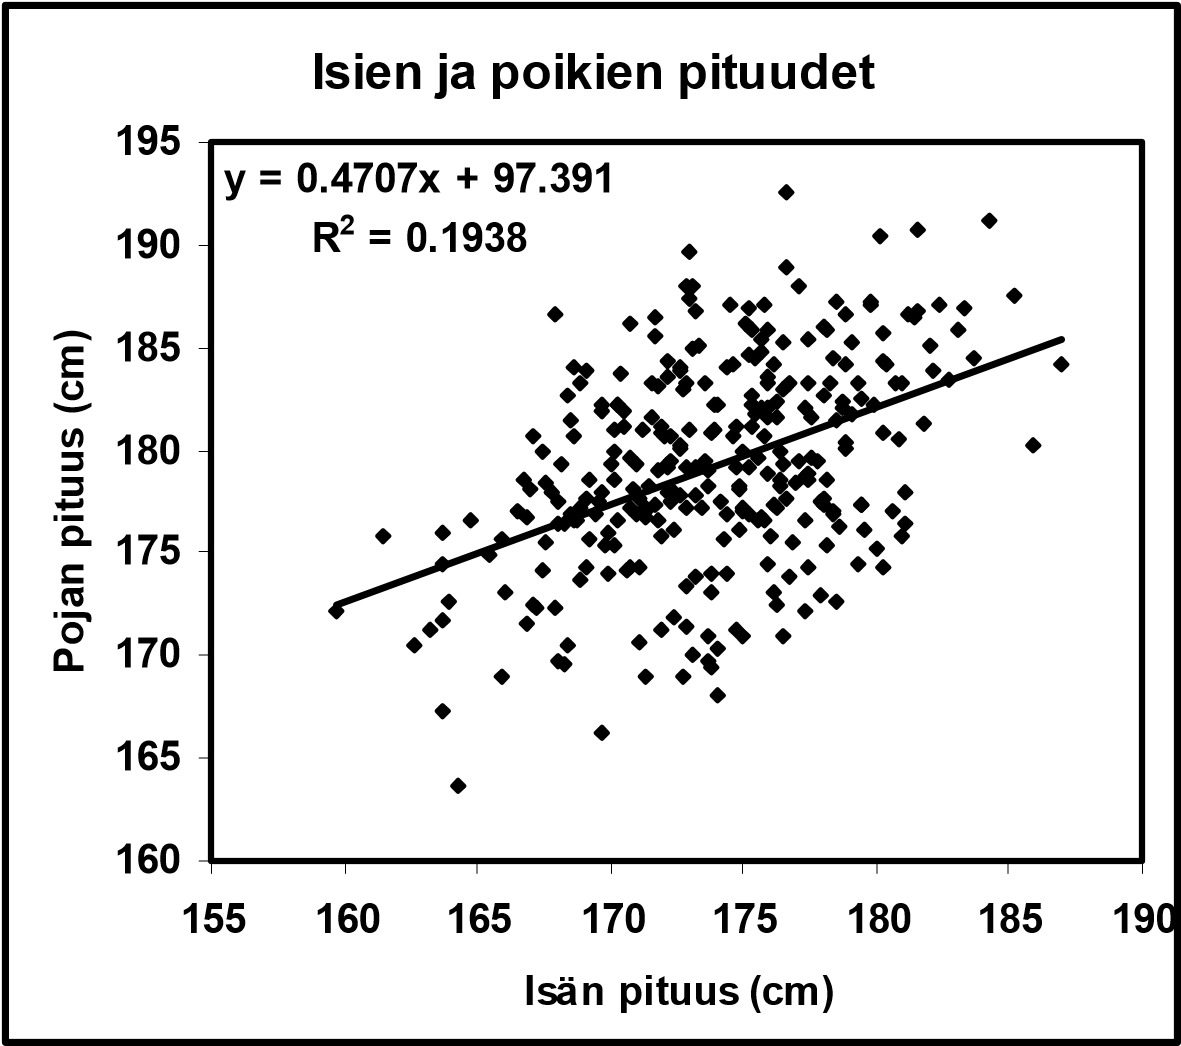
\includegraphics[width=16.4in]{images/Sovite-isien-poikien-pituudet-Mellin} \caption{Isien ja poikien pituudet: regressiosuoran sovite}\label{fig:unnamed-chunk-17}
\end{figure}

Estimoidun regressiosuoran yhtälö on (ks. oheinen kuva)
$$
y = 97.391+ 0.4707 x
$$
Suoran kulmakertoimen $\widehat{\beta}_1$ = 0.4707 tulkinta on siis, että jos isä A on 1 cm pitempi kuin isä B, isä A:n poika on keskimäärin 0.4707 cm pitempi kuin isä B:n poika.
:::

\
\

## Muita regressiomalleja {#alaluku83}

- Yksinkertaista lineaarista regressiomallia voidaan laajentaa monin tavoin monenlaisiin erilaisiin tilanteisiin.
  - Usean selittäjän lineaarinen regressiomalli: Yhden selittäjän sijaan käytetään useita selittäviä muuttujia.
  - Lineaarisen mallin sijaan malli voi olla myös epälineaarinen (epälineaarinen regressiofunktio).

- Erityisen tärkeitä laajennuksia ilmenee kun __vastemuuttuja on muuta muotoa__ mitä edellä oletetaan lineaarisissa regressiomalleissa, joissa käytännössä oletetaan että vaste on reaaliarvoinen (jokin reaaliluku). 
  - Vaste voi olla myös __diskreettiarvoinen__, kuten __binäärinen__ ($Y_i=0$ tai $Y_i=1$) tai __lukumäärä} $Y_i \in \{0,1,2,3,\ldots\}$
  - Mikäli vaste on binäärinen, niin tällöin tyypillinen tarkasteltava ja täsmennettävä tilastollinen malli on __logistinen regressiomalli__ (tunnetaan myös __logistisena regressiomallina__ tai __logit-mallina__).
  - Jos vaste on lukumäärä, niin tällöin yksi mahdollinen malliluokka on ns. __Poisson-regressiomalli__. Tässä yhteydessä oletetaan siis, että sm. $Y$ noudattaa Poisson-jakaumaa ja regressiomalli rakennetaan tämän oletuksen ympärille.
- __Vastemuuttujan roolin/luonteen selvittäminen on hyvin keskeistä tilastollista mallia rakennettaessa__. Tässä pätee samat eroavaisuudet mitkä tulevat tutuiksi todennäköisyyslaskennan kursseilla kun käsitellään diskreettien ja jatkuva-arvoisten satunnaismuuttujien jakaumia ja näihin liittyviä yksityiskohtia.

- Pitemmälle meneviä regressioanalyysin kysymyksiä käsitellään useilla myöhemmillä tilastotieteen kursseilla.
  - Perusopintojen jälkeen aineopintojen tilastollisen päättelyn kurssien [TILM3561](https://opas.peppi.utu.fi/fi/opintojakso/TILM3561/5069)- [TILM3562](https://opas.peppi.utu.fi/fi/opintojakso/TILM3562/5070) jälkeinen [TILM3588 Lineaariset ja yleistetyt lineaariset -mallit kurssilla](https://opas.peppi.utu.fi/fi/opintojakso/TILM3588/5071). Näistä jälkimmäisessä tarvitaan myös lineaarialgebran ja matriisilaskennan tietoja, joita tilastotieteen yhteydessä käydään läpi [TILM3574 Matriisilaskenta tilastotieteessä -kurssilla](https://opas.peppi.utu.fi/fi/opintojakso/TILM3574/5082).
  - Tämän jälkeen regressiomallien käsittely jatkuu useilla eri aineopintojen ja syventävien opintojen erikoiskursseilla.

<!--chapter:end:08-regressio.Rmd-->

# Tilastotieteen rooli uuden tiedon tuottamisessa {#luku9}

Tilastotieteen yhteiskunnallisesta roolista keskusteltiin luvuissa 2 ja 3. Tilastotieteen keskeinen yhteiskunnallinen rooli liittyy keskeisesti juuri uuden tieteellisen tiedon tuottamiseen: tilastotiede liittyy olennaisesti kaikkeen tieteeseen, joten ei liene yllätys että tilastotiede on jossain määrin tuttua kaikille tieteentekijöille. Tilastotiede tarjoaa pohjan uuden tiedon tuottamiselle, mutta toisaalta voitaisiin myös ajatella teoreettisen tilastotieteen ja siellä luotujen menetelmien ylipäätään mahdollistaneen uskottavan tieteenteon. Tässä luvussa emme kuitenkaan takerru tähän "muna vai kana?"-ongelmaan, vaan tarkastelemme yleisemmällä tasolla tilastotieteen roolia tieteenteossa. 

Ensiksi tarkastelemme kaikista tilastollisia menetelmiä hyödyntävistä ongelmanasetteluista löydettäviä yhteisiä elementtejä. Nämä elementit ovat niin yleisiä että niitä voidaan tarkastella ja kuvata ilman yhteyttä mihinkään yksittäiseen ongelmaan. Tämän jälkeen tarkastelemme tilastollisia menetelmiä hyödyntävän tieteellisen tutkimusprosessin eri vaiheita yleisesti. On kuitenkin mahdotonta koostaa yleisiä "tee se näin"-listoja tilastollisen tutkimuksen toteuttamiseksi, joten tarkastelemme tähän asti kurssilla käsiteltyjä asioita ja yleisiä elementtejä, jotka jokaisen tieteentekijän tulee osata ja muistaa.    

## Tilastollisen tutkimuksen yhteisiä elementtejä {#alaluku91}


1. __Satunnaisvaihtelu__
  - Satunnaisilmiöiden generoima havaintoaineisto on aina tilastollisen tutkimuksen tutkimuskohde. Täten kaikki tieteellinen tutkimus, joka koskee satunnaisvaihtelua ilmentävää aineistoa on (tai tulisi olla) tilastotieteellistä.
  - Tilastollisen tutkimuksen tavoitteena on (useimmiten) pyrkiä erottamaan satunnaisilmiön systemaattinen ja satunnainen vaihtelu. Tämä vaatii substanssiosaamisen lisäksi menetelmäosaamista sekä hyvää tilastotieteellistä intuitiota.
  - Satunnaisvaihtelun "välttämättömyys" satunnaisilmiöiden tutkimuksessa on tiedostettava ja ymmärrettävä. Tämä on tärkeää niin luotettavan tiedontuotannon kuin tutkijan oman uskottavuuden vuoksi. Tilastollisten menetelmien huonon osaamisen vuoksi tehty (ja mahdollisesti julkaistu) tutkimus voi pahimmillaan asettaa kyseisen [aiheen tutkimuksen vuosiksi väärille raiteille](https://www.nbcnews.com/science/science-news/alzheimers-theory-undermined-accusations-fabricated-research-rcna39843)!

2. __Ilmiön ja ongelman hahmottaminen järjestelmäksi__
  - Tutkimusongelman substanssiosaaminen on erityisen tärkeää tilastollisessa tutkimuksessa: on osattava tunnistaa kaikki satunnaisilmiöön mahdollisesti vaikuttavat osatekijät, jotka muodostavat satunnaisen järjestelmän.
  - Järjestelmä on joukko toisiinsa liittyviä asioita tai osia, jotka toimivat yhdessä tai ovat
jonkinlaisessa yhteydessä siten, että niiden voidaan ajatella muodostavan eriteltävissä olevan kokonaisuuden.
    - Tarvitaan kuvaus järjestelmään liittyvistä olioista, ilmiöistä ja toisaalta myös rajoituksista.
    - Lisäksi tutkimusongelman holistinen käsittely on tilastollisen tutkimuksen kannalta tärkeää: ilmiöön liittyvien tärkeiden ominaisuuksien unohtuminen tarkastelusta saattaa johtaa esimerkiksi puuttuvan muuttujan harhaan!
  - Tilastolliset menetelmät auttavat tutkijaa vastaamaan kysymyksiin siitä, mitkä tilastolliset muuttujat ovat tutkimuskysymyksen kannalta oleellisia.
    - Varsinkin nykypäivänä kun datan määrä kasvaa alati kiihtyvällä tahdilla, olemme ihmiskuntana ahdistavan informaatiotulvan edessä paikoin aseettomia: mitkä ympäröivistä ilmiöistä liittyvät toisiinsa ja miten?
    - Erityisesti teoreettisen tilastotieteen kentällä on viimeisten vuosikymmenien aikana kehitetty lukuisia edistyksellisiä menetelmiä nk. dimension pienennyksen alalla. Nämä menetelmät pyrkivät löytämään yhdenmukaisuuksia hyvin korkeaulotteisesta aineistosta, eli aineistosta jossa jokaiselta tutkimusyksiköltä mitataan jopa miljoonia eri muuttujia, kuten DNA-tutkimuksessa genomitietoa.^[Tilastotieteessä näitä menetelmiä kutsutaan monimuuttujamenetelmiksi ja niitä käsitellään tarkemmin kursseilla [TILM3704 Monimuuttujamenetelmät](https://opas.peppi.utu.fi/fi/opintojakso/TILM3704/90801) sekä [TILM3611 Monimuuttujamenetelmien jatkokurssi](https://opas.peppi.utu.fi/fi/opintojakso/TILM3611/91182)

- __Hahmottamisen vaiheet:__
  - "Todellisen" järjestelmän operationalisointi kvantitatiiviseksi kuvaukseksi järjestelmästä.
  - Tilastollisen mallin ja järjestelmästä mitattavissa olevan aineiston yhteensovittaminen   
  - Mallin antamien tulosten muotoilu sellaiseen muotoon, että ne auttavat ymmärtämään mitä aineisto kertoo todellisesta ilmiöstä

3. __Tilastollisen mallin muodostaminen ja siihen perustuva päättely__
  - Muistetaan aiempi George Boxin sitaatti: Kaikki mallit ovat vääriä, mutta jotkut ovat käyttökelpoisia.
    - Tilastollinen malli on vain kuvaus aineiston sisältämästä vaihtelusta: se ei ikinä täydellisesti ja tyhjentävästi vastaa aineiston generoinutta prosessia, mutta sitä voidaan silti käyttää kyseisen ilmiön kuvaamiseen.  
  - Kuinka saada malliin mukaan kaikki ongelmanasettelun kannalta keskeiset tekijät sellaisella tavalla, ettei oletuksiin ja abstraktioihin liittyvä informaation häviäminen kyseenalaista saatavia tuloksia?
    - Tutkimuskysymyksen kohteena olevan ilmiön taustateoria ja aiheen aiemman tutkimuskirjallisuuden hyvä osaaminen auttaa tässä.
  - Vaikutusten eritteleminen on vaikeata, mutta tilastollinen malli on yksi tapa ajatella, kuinka erittely voidaan tehdä. Esimerkkinä tällaisesta mallista mm. edellä käsitelty yksinkertainen lineaarinen regressiomalli.

4. __Synteesi__
  - Tilastollisia tarkasteluja tehdään, koska substanssitietous ei aina riitä haluttuun käyttöön. Yhdistämällä tilastotieteen keinoja sekä substanssitietoutta saadaan ongelma ratkaistua vakuuttavalla ja perustellulla tavalla.
  - Tilastollisen (soveltavan) tutkimuksen tavoitteena on tuottaa substanssitietoon perustuen ja tilastotieteen menetelmiä hyödyntäen uutta tietoa: lopputulos on menetelmä- ja substanssiosaamisen synteesi, joka tuottaa uutta substanssitietoutta (sekä joskus myös uusia ongelmia teoreettisen tilastotieteen menetelmäkehitykselle).
  - __Jokaisen tutkijan tulisi olla tilastotieteilijä ja jokaisen tilastotieteilijän tutkija__. Järkevä yhteistyö!

5. __Muita osatekijöitä:__
  - Rikas mielikuvitus. Ilman mielikuvitusta uusia yhteyksiä ei keksi etsiä.
  - Kriittinen ajattelu: Miksi tämä olisi nyt se oikea vastaus?

## Tutkimusprosessi {#alaluku92}

- Soveltavassa tilastotieteessä tutkimusongelman asettelulla on erityisen tärkeä rooli.^[Yksi soveltavan tilastotieteen osa-alue onkin [TILM3579 Kokeiden suunnittelu ja analyysi!](https://opas.peppi.utu.fi/fi/opintojakso/TILM3579/5081)] 
- Tutkimusta ei yleensä ole mahdollista jakaa täysin selvästi erillisiin ja ajallisesti tosiaan seuraaviin vaiheisiin.
  - Tutkimusprosessin vaiheet toistuvat vuorotellen ja limittäin, sillä tutkimuksen aikana tehdyt havainnot muokkaavat tutkimuksen kulkua.
  - Tutkimuksen tekeminen vaikuttaa lopulta saataviin johtopäätelmiin. Aineiston ja itse ilmiön tuntemus kasvaa tutkimuksen kuluessa.
  - Päätelmien tieteellisyyden (periaatteellinen) tarkistusmahdollisuus, ja nykyään yhä useammin jo toistettavuus, on tärkeää.

- Usein saattaa kuitenkin olla järkevää jäsentää tutkimuksessa kohdattavia tehtäviä ja vaiheita sekä niiden välisiä suhteita osana tutkimusprosessia.
  - Tutkimuksen lähtökohtana on jokin ongelma, johon tutkimuksen avulla etsitään vastausta.
  - Ilmiön ymmärtäminen: 
  - Tieto ei voi ylittää historiallisia rajojaan, joten tieteelliset teoriat ovat vain loogisia apuvälineitä, joita voidaan käyttää ilmiön tutkimuksen välineenä tai keinona sillä ehdolla, että sekä ilmiö että teoria asemoidaan ja tulkitaan suhteessa vallitseviin olosuhteisiin ja tieteelliseen keskusteluun.

- Määritelmät:
  - Ilmiöitä ei voida tutkia sellaisenaan, vaan vain niiden ilmentymien kautta käsitteiden avulla
  - Tutkimus edellyttää arkikieltä täsmällisempää kommunikaatiota, joten ongelmaan liittyvien käsitteiden huolellinen määritteleminen ja erittely on tarpeellista.
  - Määritelmät eivät korvaa empiiristä tietoa, mutta ne vaikuttavat tiedon järjestymiseen ja sen perusteella tehtävien päätelmien tekemiseen.

- Havaittava tieto
  - Yleensä ajatellaan, että todellisuudesta saadaan tietoa tavalla taikka toisella havaintoja tekemällä.
  - Havaittava tieto ei mitenkään pysty kattamaan kaikkea tutkimuskohteeseen liittyvää ja toisaalta ymmärtämiseen tarvittava havaintomaailman hahmotus tuottaa ideologisesti ja historiallisesti sitoutuneita yksinkertaistavia sekä luonteeltaan usein hyvin teoreettisia abstraktioita.

- Operationalisointi: Siirrytään teoriasta empiriaan
  - Havainnoiminen ja mittaaminen joudutaan suhteuttaamaan valittuun käsitejärjestelmään.
  - Joudutaan tekemään kompromisseja mittauksen eksaktisuus- ja systemaattisuusvaatimusten ja arkielen monimerkityksellisyyden välillä.
  - On operationalisoitava tutkimusasetelma sellaiseksi, että tutkittavasta ilmiöstä pystytään tuottamaan ongelmaratkaisun kannalta tarkoituksenmukaista tietoa.
  - Aineiston käsittely on tavallaan operationalisoinnin II vaihe. Tiedon (aineiston) muuttaminen hyödylliseksi.
  - Näkökulman kiinnittäminen:
    - Operationalisoinnin avulla siirrytään teorian tasolta empirian tasolle ja samalla tulee määritellyksi näkökulma, josta ongelmaa tarkastellaan.
    - Käsitteet ja niiden yhteyksistä esitettävät näkemykset voivat vaihtua tutkimuksen kuluessa, kunnes lopulta saavutetaan käsitteiden kyllääntymispiste
  - Numeerinen mittaus
    - Numeerisen mittauksen onnistumiseksi käsitteen muotoilu on kiinnitettävä mittariksi.
    - Numeeristen mittaustenkin tulkita edellyttää, että niitä on tulkittava siinä kontekstissa, josta ne ovat peräisin.
    - On esim. mahdollista, että esitetty kysymys ei välttämättä vastaa tutkimuskohteen ominaisuuksia.

- Aineisto
  - Aineisto edustaa tutkimuksessa empiiristä maailmaa ja se valitaan ongelmanasettelun perusteella
  - Tarvitaan systemaattinen aineisto, jonka avulla on mahdollista vastata tutkimuskysymyksiin.
  - Aineiston tuottamiseen liittyy useita valintoja, jotka implisiittisesti määräävät myös mahdolliset analyysimenetelmät.
  - Aineiston esikäsittely: 
    - Aineisto ei ole keräämiseen jälkeen yleensä koskaan suoraan käytettävissä vaan vaatii erinäistä käsittelyä 
    - Esikäsittely on operationalisoinnin II vaihe, jossa aikaisemmin tehtyjen valintojen aineistossa esiintyvät ilmentyvät sovitetaan vastaamaan ongelmankäsittelyä.

- Analyysi ja tulkinta
  - Analyysivaiheessa sopivasti käsitelty aineisto ja ongelma pyritään sovittamaan yhteen siten, että ongelmaan saataisiin perusteltu ratkaisu (selitys ja lopulta tulkinta).
  - Keskeistä on, että tehtävät oletukset sisältävät ongelmanratkaisun kannalta keskeiset tekijät sellaisella tavalla, ettei oletuksiin liittyvä informaation häviäminen kyseenalaista saatavia tuloksia.
  - Analyysien tulokset on tulkittava eli käännettävä ne takaisin empiirian kieletä teorian kielelle. Tavoitteena on siis substanssitietouteen perustuen tuottaaa uutta tietoa siten, että se lisää myös substanssitietoutta
  - Tulkinnan voi ajatella olevan operationalisoinnin käänteistapahtuma: Tutkimuksen läpiviennin sekä tulkinnan kannalta onnistunut operationalisointi ovat loppujen lopuksi yksi ja sama asia.

- Raportointi
  - Parhaimmillaan tutkimusraportti on vakuuttava, ja periaatteessa (ja toivottavasti) toiston mahdollistava, kuvaus tutkimusprosessin kaikista vaiheista, jolloin tutkija voi itse päättää haluaako uskoa saatuihin tuloksiin vai ei.
  - Keskeistä on tuoda esille, mitä uutta kyseessä oleva tutkimus on paljastunut ilmiöstä ja suhteuttaa se olemassa olevaan tietoon.
  - Tulosten perustelu: Tutkimuksen pätevyyttä ja yleistettävyyttä ja analyysin arvioitavuutta ja uskottavuutta tulisi pohtia raportissa. Tutkimuksen kuluessa tehdyt valinnat tulisi perustella tiedostaen mukaan myös omat arvopainoitteiset valinnat (ja ehkä oletuksetkin).

\
\

\textbf{Esimerkkejä tilastollisista tutkimusasetelmista}: Näitä käsitellään vielä tarkemmin myöhemmin luvussa ?? [siis seuraavassa luvussa??].

\begin{itemize}

- \textbf{Kyselytutkimukset}

\begin{itemize}

- Päätöksentekijät ja tiedotusvälineet kartoittavat säännöllisin välein suomalaisten mielipiteet erilaisista yhteiskuntaa koskevista kysymyksistä.

- Esimerkkejä:

\begin{itemize}

- Miten suomalaiset suhtautuvat NATO-jäsenyyteen?

- Miten suomalaiset suhtautuvat ydinvoiman lisärakentamiseen (osana vihreää siirtymää)?

- Mitkä ovat poliittisten puolueiden kannatusosuudet?

\end{itemize}

\begin{itemize}
\item
  Mielipiteet selvitetään kyselytutkimuksilla, joiden kohteeksi poimitaan tyypillisesti esim. noin 1000--2000 suomalaista.
\item
  Kyselytutkimuksen tavoitteena on tehdä kyselyn tulosten perusteella johtopäätöksiä mielipiteiden jakautumisesta kaikkien suomalaisten joukossa.
\item
  Miten 1000--2000 suomalaiseen kohdistetun kyselyn tulokset voidaan yleistää koskemaan kaikkia suomalaisia?
\end{itemize}

\begin{itemize}

- Kyselyn tulokset voidaan yleistää, jos kyselyn kohteiksi poimittujen suomalaisten joukko muodostaa edustavan pienoiskuvan Suomen kansasta (onnistuneen otannan idea)

- Pienoiskuva on edustava, jos mielipiteet jakautuvat kyselyn kohteiksi poimittujen joukossa samalla tavalla kuin kaikkien suomalaisten muodostamassa perusjoukossa

- Kyselyn kohteiden poiminta arpomalla on ainoa menetelmä, joka mahdollistaa edustavan pienoiskuvan saamisen

- Kyselyn kohteiden poimintaa kaikkien suomalaisten muodostamasta perusjoukosta arpomalla voidaan nähdä satunnaisotantana ja tutkimuksen kohteeksi poimittua perusjoukon osa on tässä tapauksessa (satunnais)otos

\end{itemize}

\begin{itemize}
\item
  Arvonnan käyttö kyselyn kohteiden poiminnassa merkitsee sitä, että kyselyn tulokset ovat satunnaisia seuraavassa mielessä: Jos arvontaa toistettaisiin, kysely tuottaisi (suurella todennäköisyydellä) joka kerran (ainakin jonkin verran) erilaiset tulokset, koska eri arvonnoissa kyselyyn poimittaisiin (suurella todennäköisyydellä) eri henkilöt.
\item
  Kysymyksiä:
\end{itemize}

\begin{itemize}

- Miten yhdestä otoksesta saadut ja satunnaiset kyselytulokset voidaan yleistää koskemaan koko sitä perusjoukkoa, josta otos poimitaan?

- Miten luotettava tällainen yleistys on?

\end{itemize}

\begin{itemize}
\tightlist
\item
  Vastauksia:
\end{itemize}

\begin{itemize}

- Jos kyselyn kohteiden poiminnassa on käytetty satunnaisotantaa, kyselyn tuloksiin sisältyvälle epävarmuudelle ja satunnaisuudelle voidaan muodostaa tilastollinen malli, joka mahdollistaa sekä kyselyn tulosten yleistämisen että yleistyksen luotettavuuden arvioimisen.

- Yleistyksen luotettavuutta ei pystytä arvioimaan, ellei otoksen poiminnassa ole käytetty satunnaisotantaa.

- Kyselytutkimusten suunnittelussa, toteutuksessa ja tulosten analysoinnissa sovelletaan mm. seuraavia tilastollisia menetelmiä: otanta, estimointi ja testaus.

\end{itemize}

\textbackslash end\{itemize\}

\vspace{0.75cm}

\vspace{0.75cm}

\begin{itemize}
\tightlist
\item
  Laadunvalvonta
\end{itemize}

\begin{itemize}

- Tehdas valmistaa korkealuokkaisia sulkimia kameroihin. Tehdas pyrkii siihen, että yli 90 \% sulkimista kestää vähintään 100 000 kameran laukaisua. 

- Sulkimien laadun valvonta on toteutettu seuraavalla tavalla:

\begin{itemize}

- (i) Tuotantolinjalta poimitaan arpomalla joukko sulkimia rasituskokeeseen.

- (ii) Rasituskokeessa määrätään vähintään 100 000 laukaisua kestävien sulkimien
suhteellinen osuus.

\end{itemize}

- Kokeen tavoitteena on tehdä kokeen tulosten perusteella yleisiä johtopäätöksiä sulkimien kestävyydestä.

- Miten vain osaan sulkimista kohdistetun rasituskokeen tulokset voidaan yleistää koskemaan kaikkia sulkimia?

\begin{itemize}

- Kokeen tulokset voidaan yleistää, jos rasituskokeen kohteiksi poimittujen sulkimien joukko muodostaa edustavan pienoiskuvan kaikista valmistetuista sulkimista.

- Pienoiskuva on edustava, jos sulkimien kesto jakautuu rasituskokeeseen poimittujen sulkimien joukossa samalla tavalla kuin kaikkien valmistettujen sulkimien muodostamassa perusjoukossa.

- Rasituskokeen kohteiden poiminta arpomalla on ainoa menetelmä, joka mahdollistaa edustavan pienoiskuvan saamisen.

- Rasituskokeen kohteiden poiminta kaikkien valmistettujen sulkimien muodostamasta perusjoukosta arpomalla merkitsee satunnaisotannan soveltamista ja tutkimuksen kohteeksi poimittua perusjoukon osa toimii muodostettavana (satunnais)otokseksena.

\end{itemize}

- Arvonnan käyttö rasituskokeen kohteiden poiminnassa merkitsee sitä, että koetulokset ovat satunnaisia seuraavassa mielessä: Jos arvontaa toistettaisiin, kokeesta saataisiin (suurella todennäköisyydellä) joka kerran (ainakin jonkin verran) erilaiset tulokset, koska eri arvonnoissa kokeeseen poimittaisiin (suurella todennäköisyydellä) eri sulkimet.

- Kysymyksiä:

\begin{itemize}

- Miten yhdestä kokeesta saadut ja satunnaiset koetulokset voidaan yleistää koskemaan kaikkia sulkimia?

- Miten luotettava tällainen yleistys on?

\end{itemize}

- Vastauksia:

\begin{itemize}

- Jos rasituskokeen kohteiden poiminnassa on käytetty satunnaisotantaa, kokeen tuloksiin sisältyvälle epävarmuudelle ja satunnaisuudelle voidaan muodostaa tilastollinen malli, joka mahdollistaa sekä koetulosten yleistämisen että yleistyksen luotettavuuden arvioimisen.

- Yleistyksen luotettavuutta ei pystytä arvioimaan, ellei kokeen kohteiden poiminnassa ole käytetty satunnaisotantaa.

- Kokeen suunnittelussa, toteutuksessa ja tulosten analysoinnissa sovelletaan mm. seuraavia tilastollisia menetelmiä: koesuunnittelu, otanta, estimointi ja testaus.

\end{itemize}

\end{itemize}

\textbackslash end\{itemize\}

\hypertarget{luku10}{%
\chapter{Aineisto- ja tutkimustyypit ja koeasetelmat}\label{luku10}}

\hypertarget{alaluku101}{%
\section{Tutkimustyypit}\label{alaluku101}}

\hypertarget{alaluku102}{%
\section{Tutkimusstrategiat}\label{alaluku102}}

\hypertarget{alaluku103}{%
\section{Erilaisia aineistoja ja aineistolähteitä}\label{alaluku103}}

\hypertarget{alaluku104}{%
\subsection{Rekisteriaineistot}\label{alaluku104}}

\hypertarget{alaluku105}{%
\subsection{Aikasarjat ja paneeliaineistot}\label{alaluku105}}

\hypertarget{alaluku106}{%
\subsection{Survey eli haastattelu- tai kyselytutkimus}\label{alaluku106}}

\hypertarget{luku11}{%
\chapter{Tilastollisesta ennustamisesta}\label{luku11}}

\hypertarget{alaluku111}{%
\section{Tilastollinen selittäminen vs.~ennustaminen}\label{alaluku111}}

\hypertarget{alaluku112}{%
\section{Tilastolliseen ennustamiseen liittyviä huomioita}\label{alaluku112}}

\hypertarget{luku12}{%
\chapter{Tilastotieteen kehityksen nykytrendejä}\label{luku12}}

  \bibliography{book.bib,packages.bib}

\end{document}
